\documentclass[12 pt,a4 paper, ]{scrreprt}

\setcounter{secnumdepth}{3}
\setcounter{tocdepth}{3}


%---------------------------------------------------------- 
\usepackage[utf8]{inputenc}
\usepackage[naustrian]{babel}
\usepackage{lmodern}
\usepackage[T1]{fontenc}
\usepackage{graphicx}
\usepackage{amsmath}
\usepackage{float}
\usepackage{amsmath,amssymb,amstext}

\usepackage{eurosym}
\usepackage{nicefrac}
\usepackage{units}
\usepackage{color}
%\usepackage[tight]{units}
%\usepackage[loose]{units}
\usepackage{pgfplots, pgfplotstable}
\usepackage{tikz}
\usepackage{pgfplots}

\usepackage{babelbib} %Literaturverzeichnis
\usepackage[headsepline,plainheadsepline]{scrpage2}
\pagestyle{scrheadings}
\ihead[\rightmark]{\rightmark} \chead[]{}
%\ohead[\pagemark]{\pagemark} \cfoot[]{}

\automark{chapter}
\renewcommand{\chaptermark}[1]{\markright{\ #1}}

%\usepackage[square, comma, numbers, sort&compress]{natbib}
%\usepackage{bibgerm} %Literaturverzeichnis




\pgfplotsset{width=15cm,compat=1.6}
\usepackage{pgfplots}



\begin{document}
\tableofcontents
%
\chapter{Einführung}
\section{Einleitung, Ziele und Vorgehensweise}
 

Die vorliegende Diplomarbeit entstand im Rahmen  der Forschungstätigkeit am Institut für Tragwerkplanung und Ingenieurholzbau. Sie schließt an die Arbeiten von  Kirchmayer [1] \cite{1} und  Schernberger [2] an. Im Rahmen des Forschungsprojektes "`Weitgespannte Flachdeckensysteme in Holzspanbeton – Verbundweise"'  sind ihre Arbeiten entstanden. Die Ausarbeitung von Schernberger befasst sich mit der allgemeinen Anwendung und den Einsatzgebieten des Holzleichtbetons. Kirchmayer hat anhand von Versuchsreihen das Tragverhalten- und Verformungsverhalten verschiedener Aufbauten und Verbindungsmittel untersucht.  Durch diese Versuche und Analysen ist der dargestellte Sandwichaufbau \ref{sandwich} entstanden. 



\begin{figure}[h!]
\begin{center}
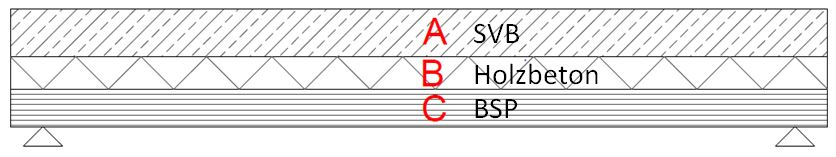
\includegraphics[scale=0.7]{Einleitung/sandwichaufbau.JPG}
\caption{Sandwichaufbau}
\label{sandwich}
\end{center}
\end{figure}

\subparagraph{Ziele und Vorgehensweise:}

Das erste übergeordnete Ziel dieser Arbeit ist die Entwicklung eines Sandwichaufbaus aus Brettsperrschichtholz (BSP), Holzleichtbeton und selbeverdichtendem Beton\,(SVB). Der SVB nimmt in dem Aufbau die Druckschicht ein, das BSP die Zugschicht und der Holzleichtbeton die Mittelschicht. Die Verbindung der unterschiedlichen Werkstoffe wird durch die Anwendung von Schrauben und einem Kleber gewährleistet. Das zweite Ziel dieser Arbeit ist die Nachrechnung der Versuchsergebnisse mit den „$\gamma$ -Verfahren“ und dem Finite Elemente Programm „Sofistik“. Es sollen die Grundlagen zur Bemessung des Sandwichaufbaus entwickelt werden. 
Zusätzlich ist eine ökonomische Betrachtung des Sandwichaufbaus zu erstellen und einen Vergleich mit den gängigen Deckensystemen zu erarbeiten.\newline Die genannten Ziele sollen mit Hilfe von den experimentellen Großbauteilversuchen erreicht werden. Dabei wird ausschließlich das Kurzzeitverhalten des Sandwichaufbaus untersucht. Die Kurzzeitdurchbiegung wurde mit l/400 begrenzt, um Reserven für Langzeitverformungen aufzubringen.




\newpage{}
Im Nachfolgenden Ablaufdiagramm ist die Vorgehensweise bei der Erstellung der Arbeit ersichtlich.

\begin{figure}[h]
\begin{center}
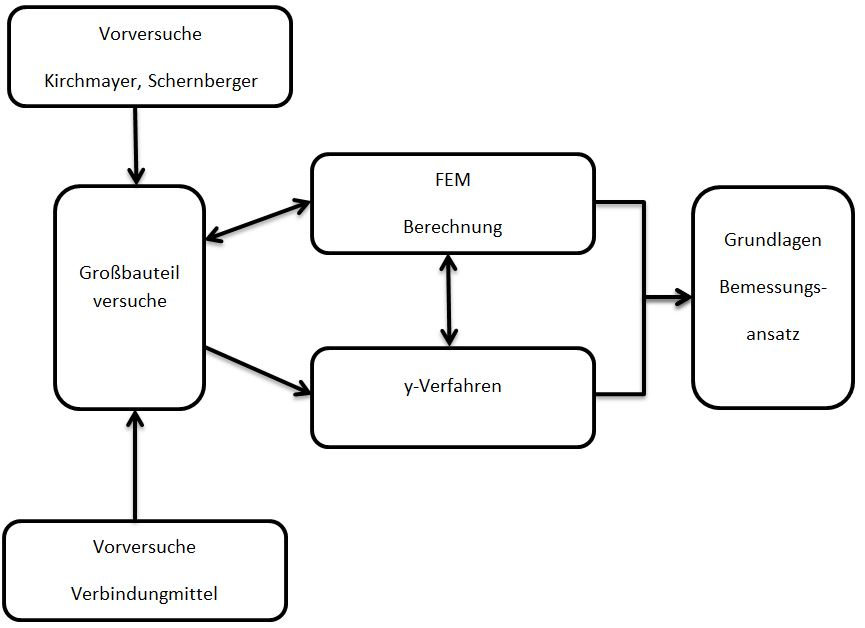
\includegraphics[scale=0.7]{Einleitung/ablauforganigramm.JPG}
\caption{Ablauforganigramm der Diplomarbeit}
\end{center}
\end{figure}




\section{Zusammenfassung der Kapitel}

\begin{enumerate}
\item Zusammenfassung von Vorarbeit 
\item Ermittlung der mechanischen Eigenschaften der Verbindungsmittel
\item Versuchaufbau und Durchführung
\item Beschreibung und Auswertung der Großbauteilversuche
\item Beschreibung der Berechnungsverfahren
\item Vergleich Berechnung Versuche und Berechnungen
\item wirtschaftliche Untersuchungen

\end{enumerate}


%\chapter{Verbindungsmittel}

Man unterscheidet zwischen metallischen Verbindungsmitteln (Drahtstifte, Schrauben, Verbindungsbeschläge) und nichtmetallischen Verbindungsmitteln (Klebstoffe, Leime, Dübel, Federn).\footnote{http://www.sign-lang.uni-hamburg.de/tlex/lemmata/l7/l708.htm,[06,2013]}



\section{Schrauben}





Die Idee war, eine Verbindung zwischen Holz und Beton herzustellen, welche die Schubkräfte abtragen kann und damit den Holzleichtbeton unterstützt. Analog zum herkömmlichen HBV - System, wurde gemeinsam mit Firma SFS das System mit langen Holzschrauben als Schubverbinder entwickelt. Die Festigkeit der Verbindungsmittel  (Verschiebungsmodul) beeinflusst das Trag- und Verformungsverhalten des nachgiebig verbundenen Sandwich-Elementes. Vorteil dieses Systems ist, dass die Schrauben ohne Vorbohren in das Holz eingebohrt werden können. Es gibt mehrere Hersteller, die in der Arbeit von Schernberger [1] aufgelistet sind, die dieses System anbieten. Es wird auch auf die Einsatzmöglichkeiten und die Vor- und Nachteile jedes Herstellers eingegangen. Die Firma hat Schraubenreihen  in verschiedensten Ausführungsvarianten und entsprechenden Schraubenlängen. Um die Auswahl der Schrauben einzugrenzen, wurden folgende Eigenschaften vorgegeben:


\begin{enumerate} 
	\item Einschraubwinkel: $45^{\circ}$
	\item Schraubenlänge: \unit[400]{mm} 
	\item Einschraubtechnik: ohne Vorbohren
	\item Keine Beschädigung der Schrauben beim durchbohren des Holzleichtbetons (Velox)
\end{enumerate}


Der vierte Punkt war aufgrund des Sandwichaufbaus noch nicht überprüft worden. Daher wurden in Zusammenarbeit mit der Firma SFS verschiedene Schraubentypen getestet. 

Die Schrauben unterschieden sich in: 

\begin{itemize}
	\item Schraubenkopfform
	\item Gewindeanordnung
	\item Schaftform
	\item Spitze
\end{itemize}

Ausgesuchte Schraubentypen: 


\begin{itemize}
	\item WR – dxL
	\item TWIN – DU dxL Sichel
	\item WT – T dxL 
	\item TWIN – DU dxL
	\item WR – T  dxL
\end{itemize}
	
\subsection{Schraubentype:	 WR – dxL}
Das Befestigungssystem WR findet hauptsächlich bei großen Querschnitten im Bereich der Verbindungen, Verstärkungen und Stahl-Holz-Anschlüsse, Anwendung. Die Schrauben sind aus Kohlenstoffstahl gefertigt. Der Schraubendurchmesser ist wählbar zwischen 9 mm oder 13 mm. Die Schrauben sind in den Längen von \unit[250]{mm} bis \unit[1000]{mm} verfügbar. Die Oberfläche der Schraube ist mit einem Durocoat überzogen, der als Korossionsschutz und als Gleitmittel fungiert.

\begin{figure}[h]
\begin{center}
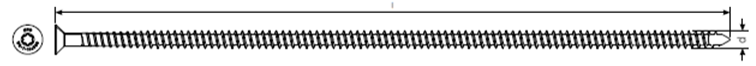
\includegraphics[scale =0.7]{Verbindungsmittel/schrauben/WR-dxL.png}
\caption{Schraubentype: WR - dxL}
\end{center}
\end{figure}


\subparagraph{Positive Eigenschaften laut Hersteller[], sind:}

\begin{itemize}
	\item sehr hohe Leitungsfähigkeit
	\item breites Anwendungsspektrum
	\item Verschraubung auch paralell zur Faserrichtung möglich
	\item keine Abminderung der Tragfähigkeit von $90^\circ  -  45^\circ$ zur Faser
	\item Verarbeitung ohne Vorbohren
	\item geringe Spaltneigung
	\item unsichtbare Verbindung
\end{itemize}


\subsection{Schraubentype: TWIN-UD dxL Sichel }
Das System TWIN DU wird seit Jahren für die Befestigung von Aufsparrendämmung auf Dächern  und hinterlüftete Fassaden verwendet. Die Schrauben sind aus Kohlenstoffstahl gefertigt. Der Schraubendurchmesser beträgt \unit[7,5]{mm} und die Schraubenlänge variiert im Bereich von \unit[160]{mm} bis \unit[480]{mm}. Die Oberfläche der Schraube ist mit einem Durocoat überzogen, der als Korossionsschutz und als Gleitmittel fungiert.

\begin{figure}[h]
\begin{center}
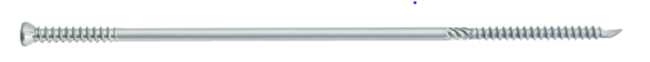
\includegraphics[scale =0.7]{Verbindungsmittel/schrauben/TWIN-UDdxLSichel.png}
\caption{Schraubentype: TWIN-UD dxL Sichel}
\end{center}
\end{figure}


\subparagraph{Positive Eigenschaften nach Angaben des Herstellers [], sind:}

\begin{itemize}
	\item Holzbohrspitze reduziert die Spaltgefahr des 	Holzes
	\item optimiertes Doppelgewinde ohne		 Gangunterschied
	\item Rändel für erleichtertes Eindrehen
	\item mehr Leistung durch angepasste 	Gewindedurchmesser
	\item hohe Traglast auf Zug und Druck dank 	Doppelgewinde
	\item minimale Wärmebrücken bei vollflächiger 	Dämmung
	\item einfache Arbeitsschritte- minimaler 	Arbeitsaufwand
	\item Dämmstärken von \unit[60]{mm} bis \unit[300]{mm} möglich
\end{itemize}


\subsection{Schraubentype: WT – T dxL }
Das Befestigungssystem WT-T ist für den universellen Einsatz im konstruktiven Holzbau in Gebrauch. Die Schrauben sind aus Kohlenstoffstahl gefertigt. Der Schraubendurchmesser ist wählbar zwischen \unit[6,5]{mm} oder \unit[8,2]{mm}. Die Schrauben sind in den Längen von  \unit[65]{mm} bis \unit[330]{mm}verfügbar. Die Oberfläche der Schraube ist mit einem Durocoat überzogen, der als Korossionsschutz und als Gleitmittel fungiert.

\begin{figure}[h]
\begin{center}
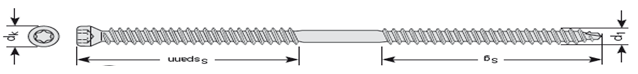
\includegraphics[scale =0.7]{Verbindungsmittel/schrauben/WT-TdxL.png}
\caption{Schraubentype: WT-T dxL}
\end{center}
\end{figure}

\subparagraph{Positive Eigenschaften laut Hersteller[], sind:}

\begin{itemize}
	\item einfache und sichere Berechnung
	\item vielfältiges Anwendungsspektrum
	\item dauerhafte Verbindung  bei hoher Tragfähigkeit
	\item schnelles, effizientes Verarbeiten ohne Vorbohren
	\item formschlüssige Verbindung  dank Doppelgewinde
	\item hoher Brandwiderstand
	\item anspruchsvolle Ästhetik dank versenkter Befestigungsmittel
	
\end{itemize}

\subsection{Schraubentype:	 WR – T  dxL}
Das Befestigungssystem WR-T ist für den universellen Einsatz im konstruktiven Holzbau in Gebrauch. Die Schrauben sind aus Kohlenstoffstahl gefertigt. Der Schraubendurchmesser ist wählbar zwischen \unit[9]{mm} oder \unit[13]{mm}. Die Schrauben sind in den Längen von  \unit[250]{mm} bis \unit[1000]{mm} verfügbar. 

\begin{figure}[h]
\begin{center}
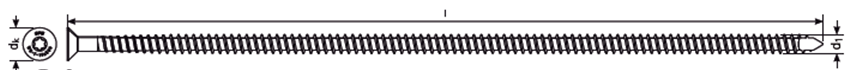
\includegraphics[scale =0.7]{Verbindungsmittel/schrauben/WR-TdxL.png}
\caption{Schraubentype: WT-T dxL}
\end{center}
\end{figure}

\subparagraph{Positive Eigenschaften nach Angaben des Herstellers [], sind:}

\begin{itemize}
	\item hohe Tragfähigkeit
	\item einfache Verarbeitung
	\item hoher Brandwiderstand der Verbindung
	\item schnelle Montage ohne Vorbohen
	\item Verbindungsmittel nicht sichtbar
\end{itemize}

\subsection{Versuchsaufbau für Schrauben}

Bei der Produktion werden zuerst die Holzbetonplatten auf die BSP geklebt und anschließend die Schrauben durch die Holzbetonplatten in die BSP eingeschraubt. Die Versuchsdurchführungen sollen sicher stellen, dass nach der Durchdringung der Holzleichtbetonschicht das Gewinde und die Spitze keinen Schaden nehmen und damit eine einwandfreie Verbindung im Holz zustande kommt. \newline Es wurden vier Lagen Veloxplatten zu je \unit[5]{cm} übereinandergelegt und mit Klemmzangen zusammengehalten. Um das Durchbohren und die anschließende Besichtigung der Schrauben zu ermöglichen, wurden die Platten auf Holzböcken gelagert.  

\begin{figure}
\begin{center}
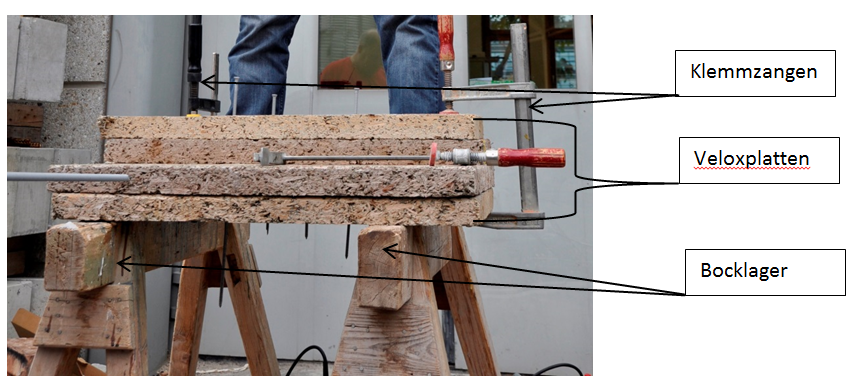
\includegraphics[scale =0.6]{Verbindungsmittel/schrauben/Schraubenversuchsaufbau.png}
\caption{ Schraubenversuchsaufbau}
\end{center}
\end{figure}

\subsection{Versuchsauswertung}

In Abbildung \ref{Schraubenauswertung} sind die Schraubenspitzen nach dem Durchbohren der Veloxplatten dargestellt. Es ist ersichtlich, dass keine der Schrauben beschädigt worden ist. Weiters war beim Einbohren der Schrauben, kein Unterschied im Kraftaufwand festzustellen. \newline

\begin{figure}[h!]
\begin{center}
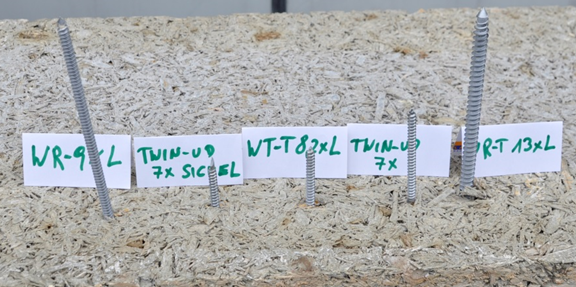
\includegraphics[scale =0.8]{Verbindungsmittel/schrauben/Schraubenauswertung.png}
\caption{ Schraubenansicht nach dem Durchbohren der vier Veloxplatten}
\label{Schraubenauswertung}
\end{center}
\end{figure}


Aufgrund der folgenden Kriterien wurde der Typ \textbf{WR – T 9\,x\unit[400]{mm}} ausgewählt.
Um über den gesamten Einbohrvorgang eine Führung zu gewährleisten, wurde eine Gewindeanordnung über die gesamte Schraubenlänge bevorzugt. Zusätzlich kann durch das Gewinde ein besserer Auszugswiderstand aus dem Beton gewährleistet werden. Die Bandbreite der Schraubenlänge beträgt \unit[250]{mm} bis \unit[1000]{mm}.
Die Spitze war ein weiteres Entscheidungskriterium, hierbei wurde darauf geachtet, dass sich die Schraube problemlos mit einem einfachen Hilfsmittel (Hammer) ansetzen lässt. 
Der Schraubenkopf besitzt eine große Fläche, somit wird ein guter  Verbund mit dem Beton erreicht. 





\section{Kleber}
Unter Kleben versteht man: Fügen gleicher oder ungleicher Werkstoffe unter Verwendung eines Klebstoffes.[(nach EN DIN 923,[])] 

Klebstoffe sind nichtmetallische Stoffe, die Fügeteile durch Flächenhaftung und innere Festigkeit(Adhäsion und Kohäsion) verbinden.(nach EN DIN 923,[])


\subsection{Einteilung}

Die Einteilung der Klebestoffe wird in Habenich[] auf zwei Arten angeführt. Zum einen auf der chemischen Basis und nach dem Abbindemechanismus. 
\begin{figure}[h]
\begin{center}
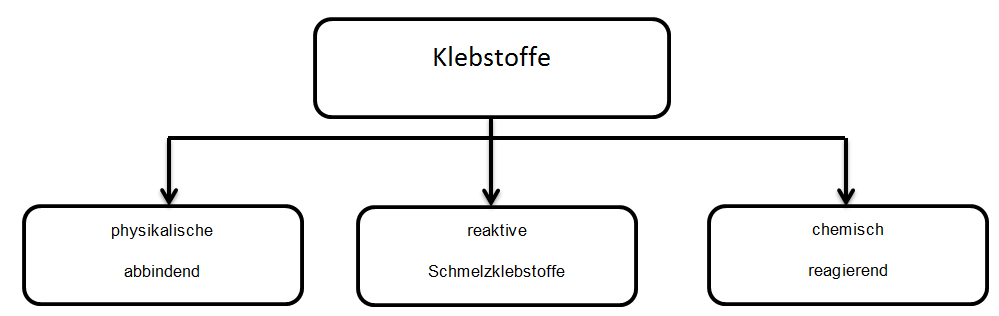
\includegraphics[scale =0.6]{Verbindungsmittel/kleber/einteilungderklebstoffe.png}
\caption{ Einteilung der Klebstoffe nach dem Abbindemechanismus, []}
\label{Einteilung der Kelbstoffe}
\end{center}
\end{figure}


\subsection{Vor- und Nachteile der Klebverbindungen}

Habenich [] hat die Vor- und Nachteile des Klebens gegenüber Schweißen, Löten, Schrauben, und Nieten beschrieben. 
\newline{}

\textbf{Vorteile von Klebungen,[4, Tabelle 7.1]}
\begin{itemize}
	\item gleichmäßige Spannungsverteilung senkrecht zur Belastungsrichtung 
	\item keine Thermische Gefügebeeinflussung
	\item kein thermisch bedingter Bauteilverzug
	\item Verbindungsmöglichkeit für unterschiedliche Materialkomponenten
	\item Gewichtsersparnis, Leichtbau
	\item Verbingungsmöglichkeit für sehr wärmeempfindliche Werkstoffe
	\item Festigkeitserhöhung in Verbindung mit Schrauben
	\item hohe dynamische Festigkeit, hohe Schwingunsdämpfung
	\item Möglichkeit zur Automatisierung
\end{itemize}


\textbf{Nachteile von Klebungen, [4, Tabelle 7.2]}

\begin{itemize}
	\item Einfluss der Zeit auf den Verfahrensablauf
	\item Oberflächenvorbehandlung der Fügeteile
	\item begrenzte thermische Frombeständigkeit
	\item sorgfältige Prozesskontrolle
	\item Alterungsabhängigkeit der Klebschicht und Grenzschicht
	\item aufwendige Kontrollverfahren
	\item geringe Schälwiderstände, Kriechneigung
	\item begrenzte Reparaturmöglichkeiten
	\item aufwendige Festigkeitsberechnungen
	\item Demontage von Klebungen
	\end{itemize}


\section{Kleberversuche}

Die Kleberversuche wurden unternommen, um der Probleme der Verarbeitung, der Klebermenge, der Kosten und das Verbundverhalten des Klebers mit den Sandwichschichten zu ermitteln.\newline
Daher wurde auf folgende Eigenschaften der Kleber eingegangen :	

\begin{itemize}
	\item Klebermenge
	\item Haftzug
	\item Verarbeitbarkeit
	\end{itemize}




\subsection{Ermittlung des Klebermenge mit der Sandfleckmethode}

Mit der Sandfleckmethode wird die Rauigkeit von porösen Materialien bestimmt  
und mit einem Formelwerk der Bedarf ermittelt.

\paragraph{Durchführung}
Es wird 15 $g$ feiner Sand mit einer Körnung von \unit[0,1]{mm} bis \unit[0,2]{mm}  in einen kleinen Behälter gefüllt. Anschließend wird der Sand auf dem porösem Material aufgebracht [Abbildung \ref{sandfleck}]und mit Hilfe eines Stempels kreisförmig verteilt. Somit werden die oberflächigen Hohlräume (Poren) ausgefüllt. Der mittlere Durchmesser des „Sandflecks“ wird anschließend gemessen [Abbildung \ref{sandfleckmessen}]. Anhand des Durchmesser und des Volumens wird die Rautiefe bestimmt. Mit Rautiefe und zusätzlichen Parametern (Spachtelfaktor, Schichtdicke) wird der Kleberverbrauch berechnet.

\begin{figure}[h]
\begin{minipage}[hbt]{7cm}	
	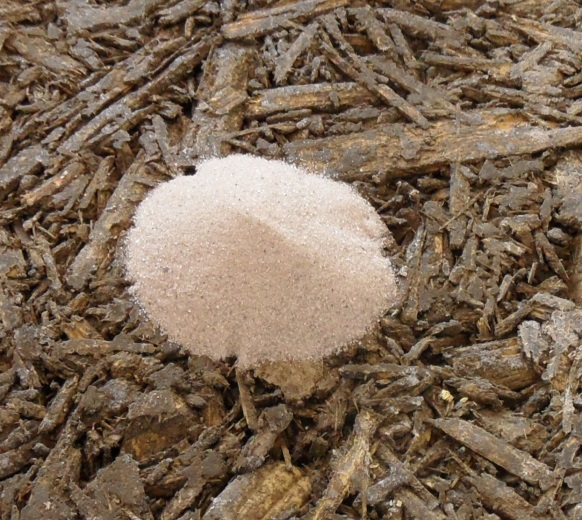
\includegraphics[width=7.7cm]{Verbindungsmittel/kleber/sandfleck.png}
	\caption{Aufgeschütteter Sandfleck auf der Veloxplatte}
	\label{sandfleck}
\end{minipage}
\hfill
\begin{minipage}[hbt]{7cm}
	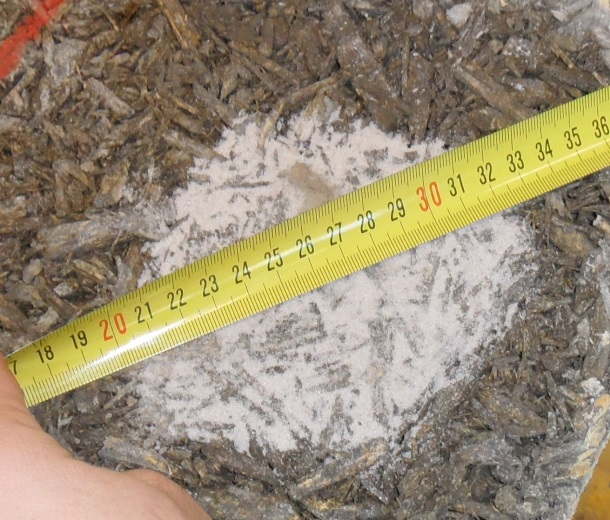
\includegraphics[width=8cm]{Verbindungsmittel/kleber/sandfleckmessen.png}
	\caption{Ermittlung des mittleren Durchmessers,$D=\unit[11]{cm}$}
	\label{sandfleckmessen}
\end{minipage}
\end{figure}
\paragraph{Berechnng des Kleberbedarfs: SikaTop-109 ElastoCem, nach Sika}

\textbf{Angaben:}
\begin{center}

\begin{itemize}
\item mittlere Durchmesser:D=\unit[11]{cm}
\item Sandvolumen:	V= \unit[0,01]{L}
\item Dichte:	$\rho$=1.60\, $\dfrac{kg}{L}$
\item Trägerabmessung(l x b):	7,40\, x\, 0,50\, m 
\end{itemize}
\end{center}


\textbf{Annahmen:}

\begin{itemize}
\item Spachtelfaktor:	$f_{sp}=\dfrac{2}{3}$  
\item Schichtdicke:		$f_{sd}=$\unit[3]{mm}
\end{itemize}
 

\subparagraph{Berechnung der Rauigkeit:}
\begin{equation}
r=\dfrac{V*4}{\pi*d^{2}}=\unit[1,05]{mm}
\end{equation}

\subparagraph{Kleberbedarf pro Fläche}

\begin{equation}
b_{K}= 2\dfrac{kg}{L}*f_{sd}=\unit[6]{\dfrac{kg}{m^{2}}}
\end{equation}

\subparagraph{Kleberbedarf für Porenverschluss}

\begin{equation}
b_{K,P}=r*\rho*f_{sd}= \unit[1,12]{\dfrac{kg}{m^{2}}}
\end{equation}

\subparagraph{Bedarf für BSP-Velox-Schichte}

\begin{equation}
B_{BSP-Velox}=Kb*l*b=\unit[22,22]{kg}
\end{equation}

\subparagraph{Bedarf für Velox-Velox-Schichte}

\begin{equation}
B_{Velox-Velox}=(Kb+Kp)*l*b=\unit[26,35]{kg}
\end{equation}


\subparagraph{Benötigter Kleber für den gesamten Träger}

\begin{equation}
B_{gesamt}=B_{BSP-Velox}+2*B_{Velox-Velox}=\unit[74,91]{kg}
\end{equation}







\section{Haftzugprüfung}\label{{sec:Haftzugprufung}}
Um den Haftverbund der Kleber mit der Veloxplatte zu untersuchen, wurde die Haftzugprüfung angewendet. In der Abbildung \ref{Z16E} ist die Prüfeinheit (Dynameter Z16E) dargestellt.

\begin{figure}
\begin{center}
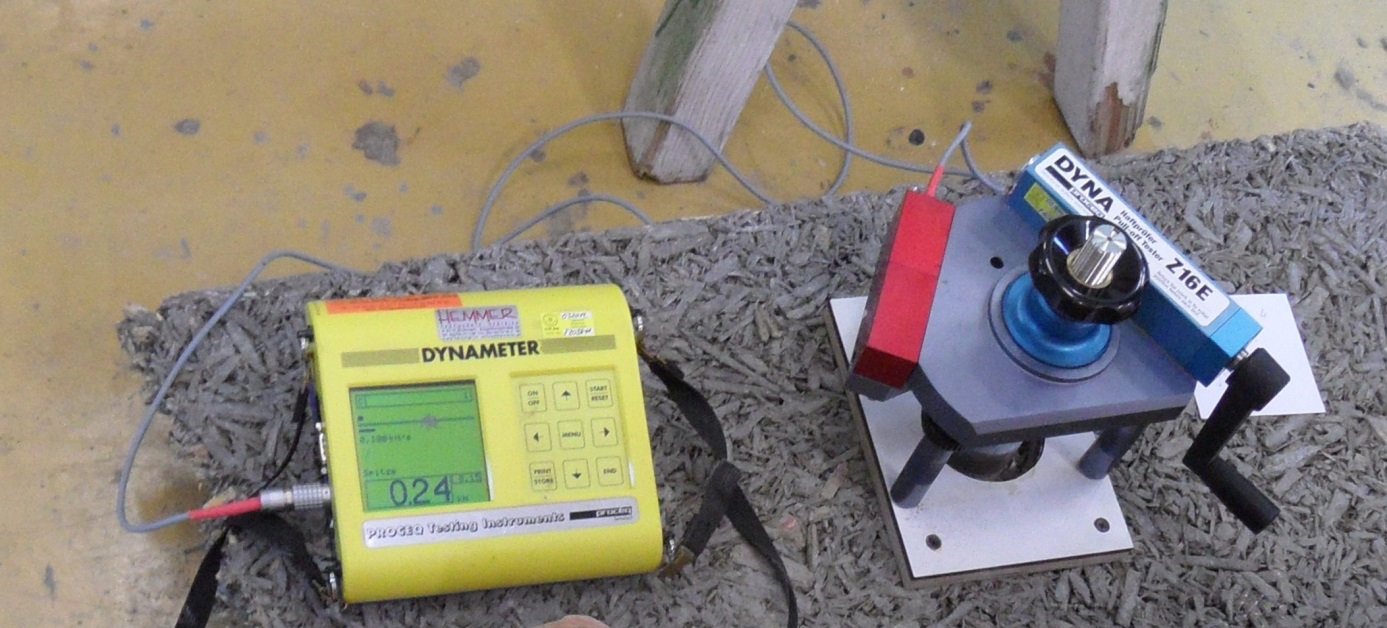
\includegraphics[scale =0.7]{Verbindungsmittel/kleber/Z16E.jpg}
\caption{ Prüfgerät:Dynameter Z16E, Ausgabeeinheit und Messeinheit}
\label{Z16E}
\end{center}
\end{figure}

\newpage{}
\subsection{Versuchsvorbereitung}
\subparagraph{Anmischen:}
Die zu testenden Kleber basieren alle auf einem 2-Komponenten-System. Daher mussten die Komponenten nach dem vom Hersteller  angegebenen Mischverhältnis abgemischt werden. Um eine einheitliche Masse zu erhalten, wurden die zwei Komponenten mit einem Quirl vermischt. 

\subparagraph{Auftrag des Klebers:}
Zuerst wurden die oberflächigen Poren vom Holzbeton (Velox) mit Hilfe einer Spachtel verschlossen. Anschließend wurde der Kleber mit einer Zahnspachtel aufgetragen. Die Kleberproben hatten eine Aushärtezeit von einer Woche.

\subparagraph{Aufkleben des Stempels}

Im ersten Schritt wurden 3 Kernbohrungen auf jeder Probe gebohrt. Um den Aushärteprozess des schnellhärtenden Epoxidklebers (Uhuplus oder X60) zu beschleunigen, wurden die Stempel mit einen Heißluftfön vorgewärmt. Anschließend wurde der Epoxidkleber abgemischt und auf die Kernbohrungen der Proben aufgetragen. Der vorgewärmte Stempel wurde mit geringem Kraftaufwand auf den Epoxidkleber gepresst. Die Aushärtezeit für den KLeber (UHUplus) betrug \unit [15]{min}.


\subsection{Versuchsdurchführung}

Zuerst wurde der Bolzen in das Gewinde des Stempels eingedreht. Anschließend wurde die Messeinheit des Prüfgeräts über der Probe positioniert und der Bolzen in die Einkerbung eingefädelt. Das Aufbringen der gleichmäßigen Kraft wurde manuell mit der Handkurbel verrichtet. Nach dem Versuch wurde die gemessene Maximalkraft am Ausgabeeinheit abgelesen.




\begin{figure}
\begin{center}
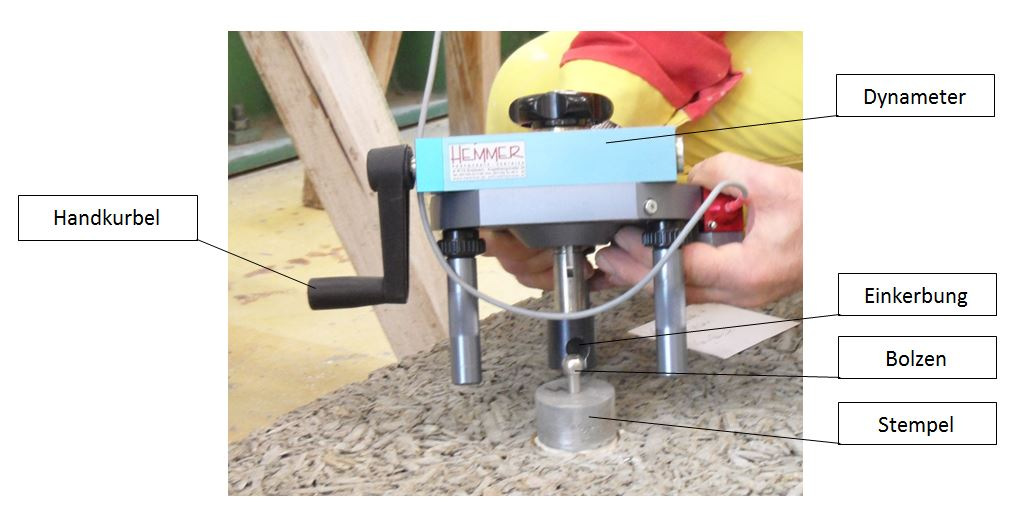
\includegraphics[scale =0.6]{Verbindungsmittel/kleber/dynameter.jpg}
\caption{ Dynameter Z16E: Hauptbestandteile der Messeinheit }
\label{dynameter}
\end{center}
\end{figure}




\section{Kleberversuchsreihe 1}

Beim ersten Bauteilversuch traten einige Probleme bei der Verarbeitung des Kleber Sikadur 31 auf. Dieser Kleber wurde auch von Kirchmayer bei seinen Verbundversuchen verwendet. Da der Aufbau von Kirchmayer kleiner war und somit auch die Klebermenge geringer, hatte er keine Probleme bei der Verarbeitung. Der Kleber entwickelt bei großen Mischmengen eine schnelle Aushärtezeit und war beim Auftragen über den gesamten Träger sehr schwer zu verarbeiten. Um eine bessere Verarbeitung zu gewährleisten und wirtschaftlichere Kleber zu verwenden, wurden alternative und kostengünstigere Kleber untersucht. 


In Abstimmung mit der Firma Sika wurde die Anwendung abgeklärt und folgende Kleber getestet:
\begin{itemize}
\item SikaFloor 161
\item SikaTop-109 ElastoCem
\item SikaForce 7710 L35
\end{itemize}




In den nachfolgenden Abbildungen \ref{1Versuchsplatte} - \ref{3Versuchsplatte} sind die getrockneten Kleber und die aufgeklebten Prüfstempel ersichtlich. In Abbildung \ref{4Versuchsplatte} ist die Veloxplatte dargestellt. Um einen Referenzwert zu den Versuchsergebnissen mit Kleber zu erhalten, wurde  die Veloxplatte ohne einen Kleber einer Haftzugprüfung unterzogen.

\begin{figure}[h]
\begin{minipage}[hbt]{7cm}	
	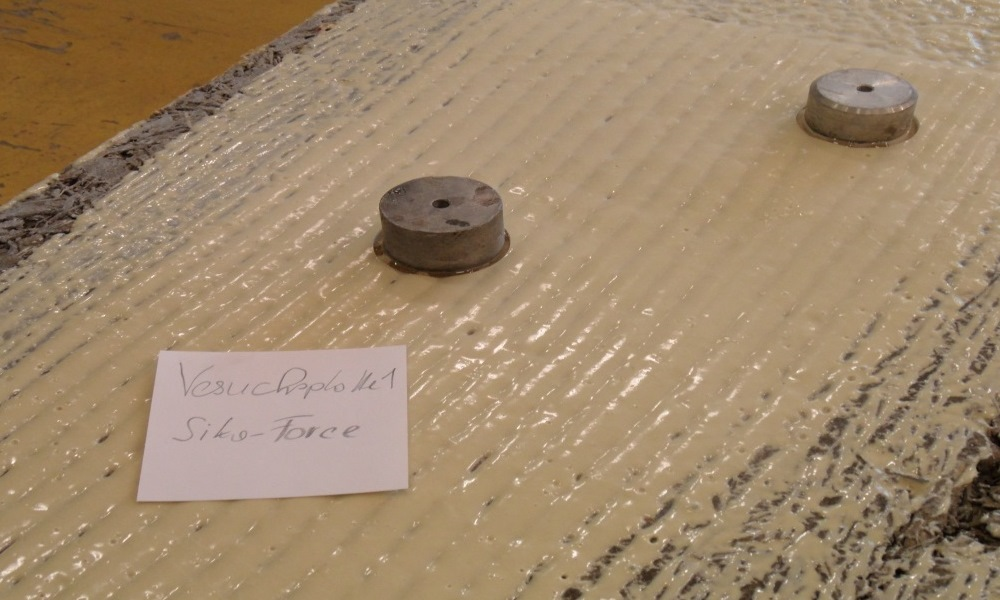
\includegraphics[width=7cm]{Verbindungsmittel/kleber/1Versuchsplatte.jpg}
	\caption{Versuchsplatte (SikaForce-7710 L35)}
	\label{1Versuchsplatte}
\end{minipage}
\hfill
\begin{minipage}[hbt]{7cm}
	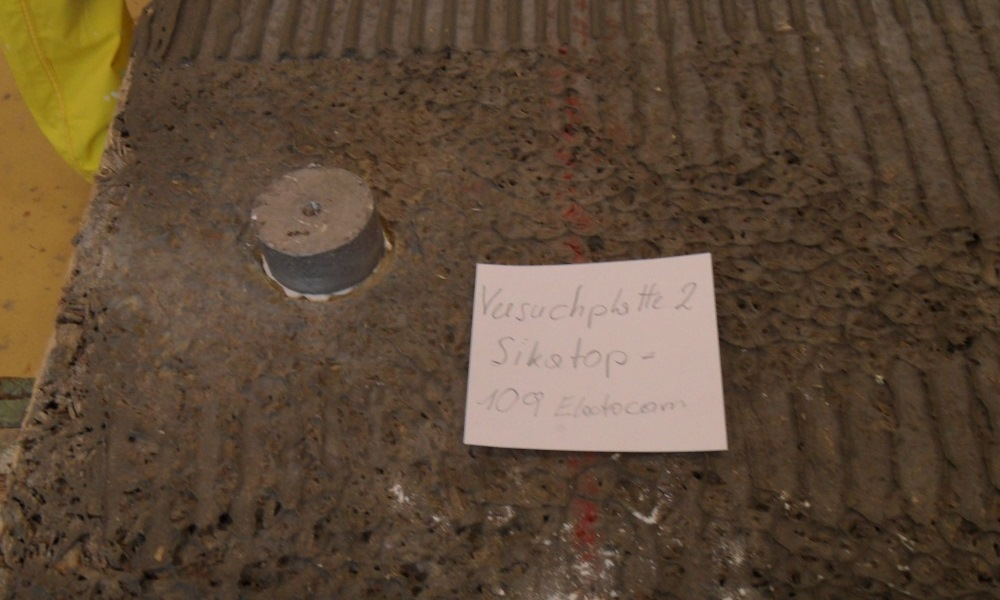
\includegraphics[width=7cm]{Verbindungsmittel/kleber/2Versuchsplatte.jpg}
	\caption{Versuchsplatte (SikaTop-109 ElastoCem)}
	\label{2Versuchsplatte}
\end{minipage}
\end{figure}


\begin{figure}[h]
\begin{minipage}[hbt]{7cm}	
	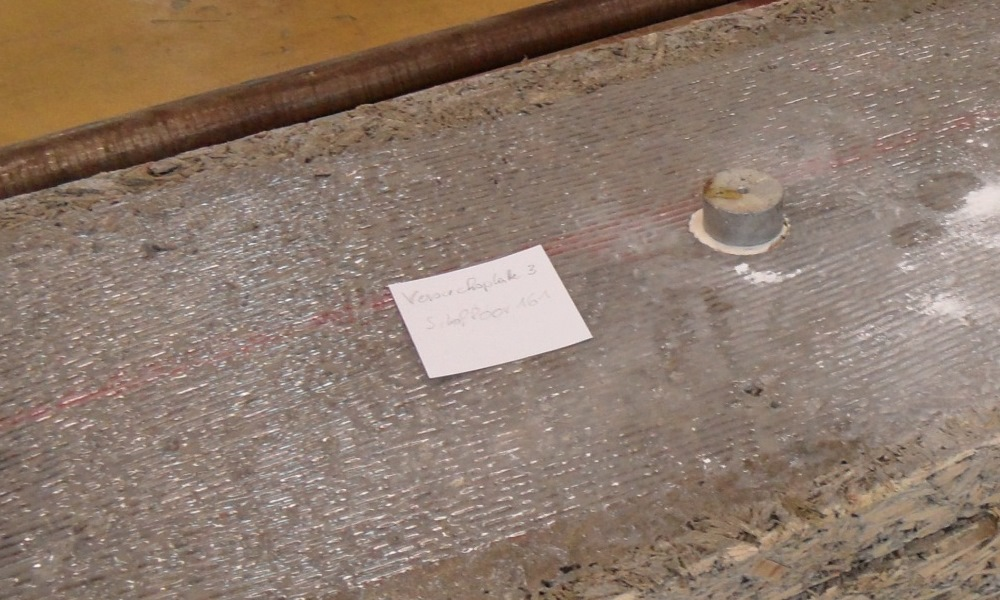
\includegraphics[width=7cm]{Verbindungsmittel/kleber/3Versuchsplatte.jpg}
	\caption{Versuchsplatte (SikaFloor-161))}
	\label{3Versuchsplatte}
\end{minipage}
\hfill
\begin{minipage}[hbt]{7cm}
	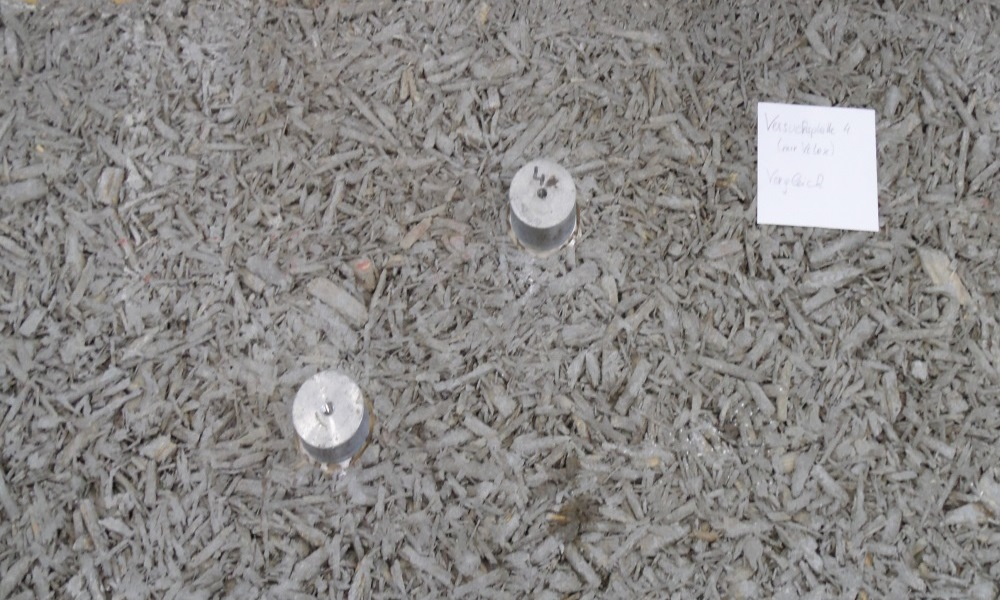
\includegraphics[width=7cm]{Verbindungsmittel/kleber/4Versuchsplatte.jpg}
	\caption{Versuchsplatte (ohne Kleber)}
	\label{4Versuchsplatte}
\end{minipage}
\end{figure}





\begin{table}[h!]
\caption{Messergebnisse und Auswertung der Kleberversuchsreihe\,1}
\begin{center}

\begin{tabular}{|c|c|c|c|c|} \hline
Versuchsplatte & Kraft & Durchschnitt & Spannung &Durchschnitt \\

	& [kN] & [kN] & [N/mm$^{2}$] & [N/mm$^{2}$] \\
	\hline\hline
 \cline{2-2} 1 Versuch: SikaForce-7710 L35  & 1,47 & & 0,75& \\\cline{2-2}&1,56 &1,45 &0,79 &0,74 \\\cline{2-2}&1,32 & &0,67 & 
\\\hline\hline

 \cline{2-2} 2 Versuch: SikaTop-109 ElastoCem  & 0,74 & & 0,38& \\\cline{2-2}&0,77 &0,77 &0,39 &0,39 \\\cline{2-2}&0,80 & &0,41 & 
\\\hline\hline

 \cline{2-2} 3 Versuch: SikaFloor-161  & 2,11 & & 1,07& \\\cline{2-2}&1,82 &2,04 &0,93 &1,04 \\\cline{2-2}&2,20 & &2,12 & 
\\\hline\hline


 \cline{2-2} 4 Versuch: nur Velox  & 0,84 & & 0,43& \\\cline{2-2}&0.80 &0,82 &0,41 &0,42 
\\\hline

\end{tabular}
 \label{tab:1 kleberversuche}

\end{center}
\end{table}



\newpage

\subparagraph{Zwischenfazit:}


Die Kleber SikaForce-7710 L35 und SikaFloor 161 haben sehr gute Klebeeigenschaft, welche anhand der Versuchsergebnisse (Tabelle\, \ref{tab:1 kleberversuche}) erkennen kann. Es versagte bei den beiden nicht der Kleber sondern das Velox. Die innere Festigkeit von Velox war geringer, als die des Klebers. 

Beim Kleber SikaTop-109 ElastoCem hat nicht das Velox versagt, sondern der Kleber. Es ist zu vermuten, dass das Velox eine höhere innere Festigkeit als der Kleber hat. Da dieser Kleber auf Zement basiert, ist eine Aushärtezeit von \unit [28]{Tagen} erforderlich, damit er seine Endfestigkeit erreicht.  Somit werden die Ergebnisse der Haftzugprüfung nach einer Woche unterschätzt.  Die Haftzugfestigkeit wird im Produktdatenblatt [] der Fa. Sika mit \unit[0,7]{$N/mm^{2}$} geführt. Daher ist zu erwarten, dass die innere Festigkeit des Klebers mit längerer Aushärtezeit ansteigt.
Aufgrund der einfachen Vorbereitung und der guten Verarbeitung haben wir uns für diesen Kleber entschieden. Durch die Verwendung des Aufbetons muss eine entsprechende Aushärtezeit für den Bauteil vorgesehen werden und ergibt daher  keine Einschränkung für den Kleber. 

\section{Kleberversuchsreihe 2}

Es wurden nach dem zweiten Bauteilversuch weitere Kleberversuche durchgeführt. Der Grund dafür war, dass der Kleber SikaTop-109 ElastoCem schon beim Einheben in die Prüfeinrichtung Beschädigungen aufwies. Es waren Teile der Veloxschichten nicht mehr miteinander verbunden. Dies war vor allem bei den Auflager ersichtlich. Durch den nicht vorhandenen Verbund waren auch Zugrisse in der Aufbetonschicht (ca. \unit[2.0]{m} von den Auflagern) aufgetreten. In den Abbildungen \ref{lagera} und \ref{lagerb} ist dargestellt, in welchem Ausmaß sich die Veloxplatten von einander lösten. Die Messlatte war \unit[30]{cm} lang und die Unterteilungen kennzeichnen \unit[5]{cm} Schritte.  

\begin{figure} [h]
\begin{minipage}[hbt]{7cm}	
	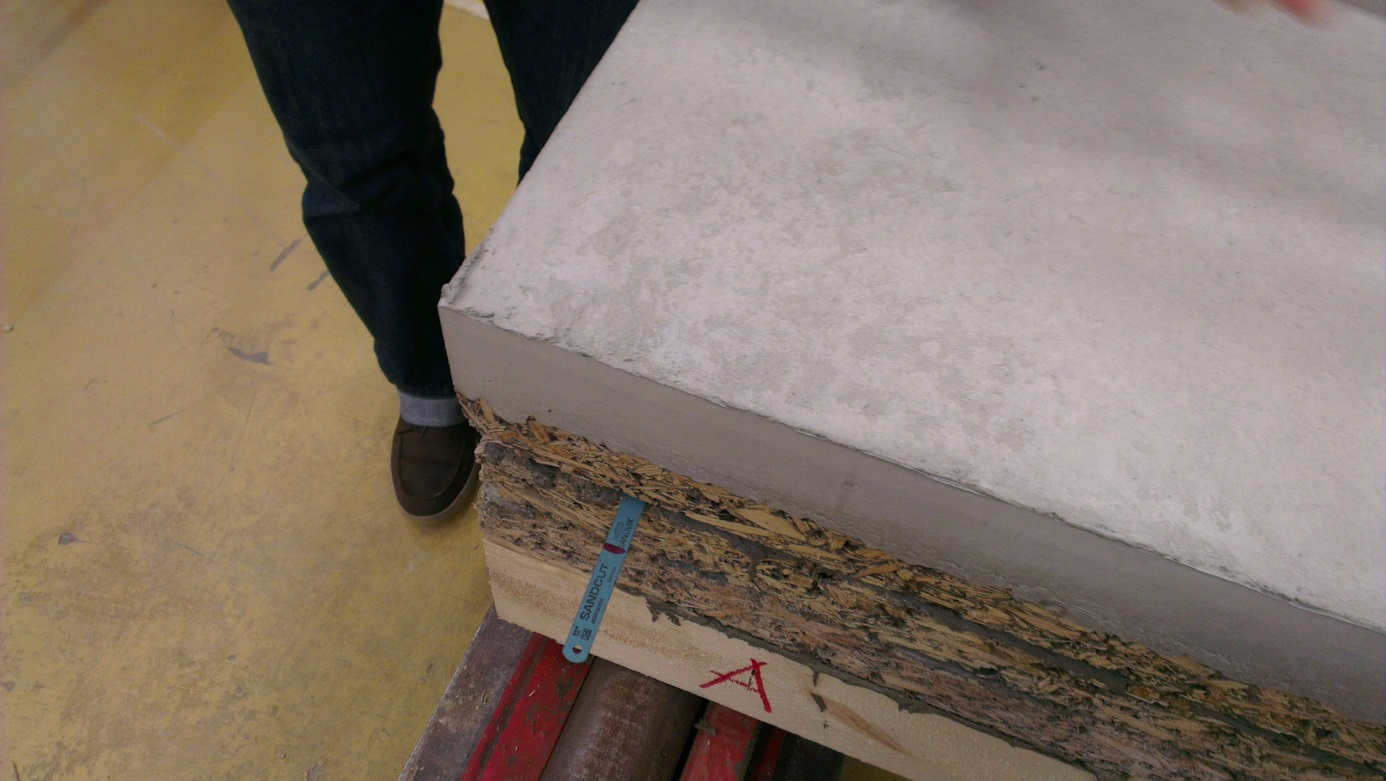
\includegraphics[width=7.7cm]{Verbindungsmittel/kleber/lagera.jpg}
	\caption{Fehlerhaftere Verbung beim Auflager A}
	\label{lagera}
\end{minipage}
\hfill
\begin{minipage}[hbt]{7cm}
	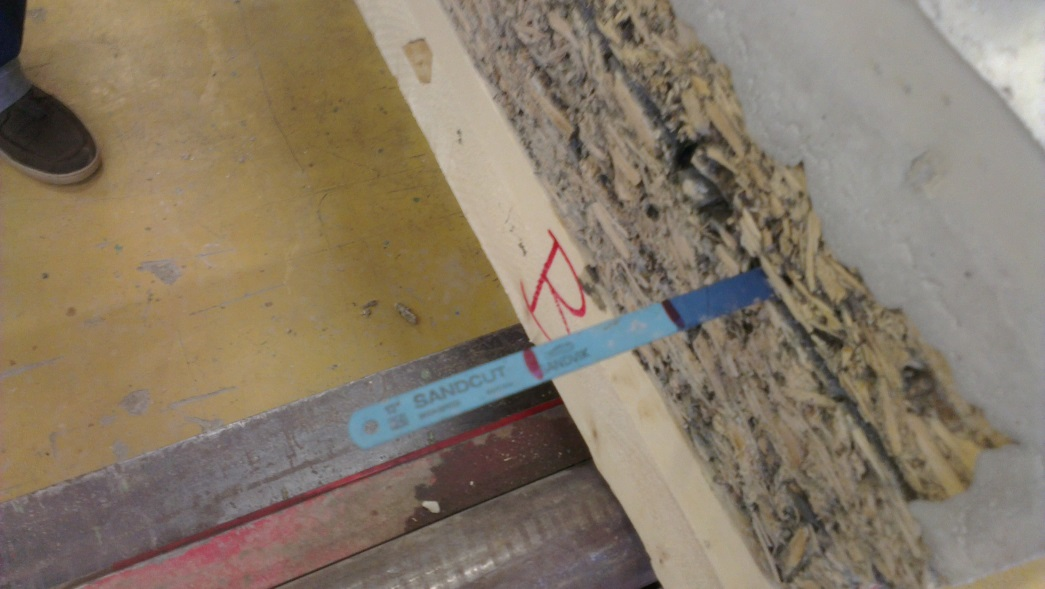
\includegraphics[width=8cm]{Verbindungsmittel/kleber/lagerb.jpg}
	\caption{Fehlerhaftere Verbung beim Auflager B}
	\label{lagerb}
\end{minipage}
\end{figure}



Es wurde wieder in der Absprache mit der Firma Sika ein  2-Komponenten-Kleber  SikaTop-107 Seal gewählt. Dieser Kleber hat etwa die doppelte Festigkeit (lt.Produktdatenblatt[]) des Klebers SikaTop-109 ElastoCem. Er besitzt die gleichen Verarbeitungs-und Kostenvorteile (siehe Kapitel\,8) wie der Kleber SikaTop-109 ElastoCem. Um das Verbundverhalten des Klebers mit dem BSP zu untersuchen, wurden Versuchsproben erstellt. Der Aufbau und Ablauf entsprach gleich der Versuchsreihe\,1.
In Abbildungen \ref{holz-kleber} und \ref{velox-kleber} sind die Versuchskörper für das BSP (H1-H3) und für das Velox (V1-V3) dargestellt.


\begin{figure} 
\begin{minipage}[hbt]{7cm}	
	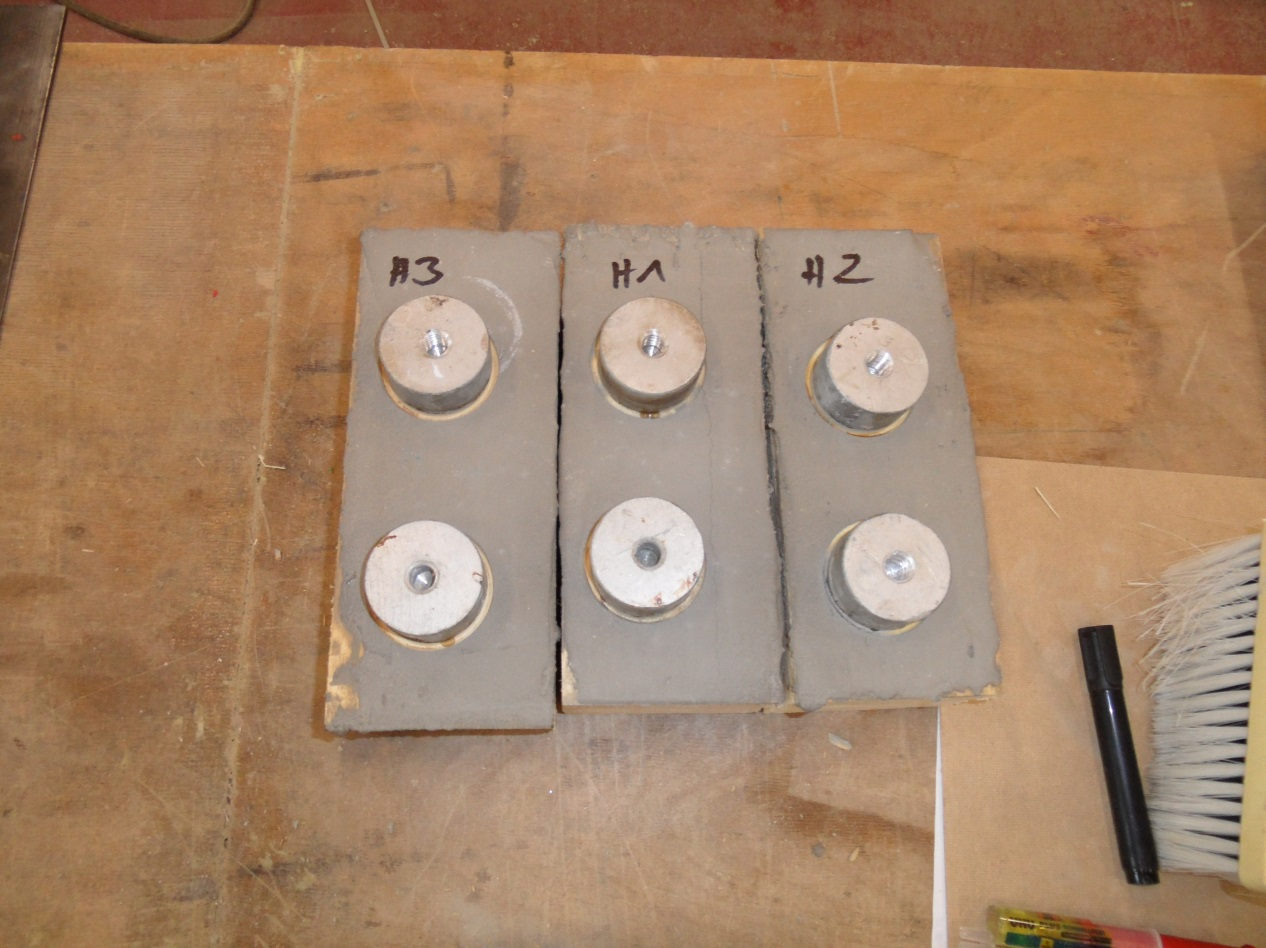
\includegraphics[width=7.7cm]{Verbindungsmittel/kleber/holz-kleber.jpg}
	\caption{Versuchskörper: Sikatop 107 auf Holz}
	\label{holz-kleber}
\end{minipage}
\hfill
\begin{minipage}[hbt]{7cm}
	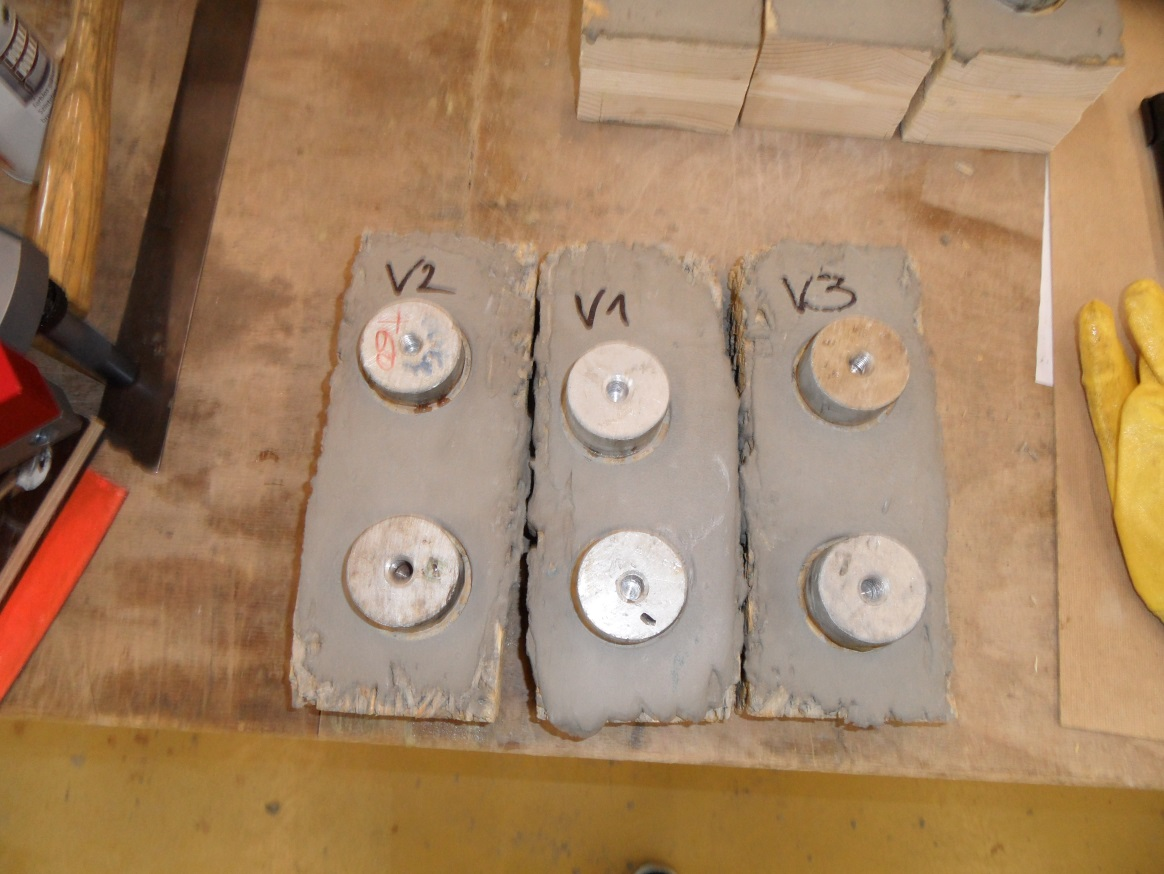
\includegraphics[width=8cm]{Verbindungsmittel/kleber/velox-kleber.jpg}
	\caption{Versuchskörper: Sikatop auf Velox}
	\label{velox-kleber}
\end{minipage}
\end{figure}

Der Kleber SikaTop-107 Seal wurde mit dem Mischverhältnis von 1:4,5 abgemischt und auf die Probenkörper aufgetragen. Vor dem Auftragen wurde das Holz und das Velox noch befeuchtet, da beim Aushärten des Klebers ein Feuchtigkeitstransport in das Holz stattfindet. Um einen Vergleich zu der ersten Versuchsreihe zu erhalten, härtete der Kleber eine Woche aus. Der Ablauf der Haftzugprüfung erfolgte ident zu den vorigen Versuchen.

In Abbildung \ref{probenbild} sind die Proben mit den dazugehörigen Bruchflächen dargestellt. Einige Stempel weisen rot markierte Stellen auf, da in diesem Bereich der schnellhärtende Epoxidkleber (UHU-Plus) nicht geklebt hat. Daher wurde bei der Spannungsberechnung die Fläche (A = \unit[19,64]{$cm^{2}$}) um diesen Abminderungsanteil verringert. [Tabelle:\ref{tab:2.1 kleberversuche}]

\begin{figure}
\begin{center}
\includegraphics[scale =0.8]{Verbindungsmittel/kleber/Probenbild.jpg}
\caption{Bruchflächen der Proben (SikaTop 107); rote Markierung: fehlender Verbund zwischen schnellhärtenden Epoxidkleber und Stempel}
\label{probenbild}
\end{center}
\end{figure}





\begin{table}
\caption{Auswertung der Kleberversuchsreihe\,2, BSP}
\begin{tabular}{|c|c|c|c|c|c|} \hline
\multicolumn{6}{|c|}{SikaTop-107 auf BSP} \\\hline
Versuchsplatte & Kraft & Durchschnitt & Spannung & Abminderung & Durchschnitt \\
	& [kN] & [kN] & [N/mm$^{2}$] & [\%] & [N/mm$^{2}$] \\
	\hline\hline
\cline{2-2} 1 Versuch: H1  & 1,25 & & 0,85& 25,0& \\\cline{2-2}&0,99 & 1,12 &1,51 & & 1,18
\\\hline\hline

\cline{2-2} 2 Versuch: H2  & 1,46 & & 1,30& 43,0& \\\cline{2-2}&1,86 & 1,66 &0,95 & & 1,13
\\\hline\hline

\cline{2-2} 3 Versuch: H3 & 1,07 & & 0,62&12,0 & \\\cline{2-2}&2,27 &1,67 &1,16 & 5,0 & 0,89 
\\\hline

\end{tabular}
 \label{tab:2.1 kleberversuche}
 \end{table}

\begin{table}
\caption{Auswertung der 2 Kleberversuchsreihe, Velox}
\begin{center}


\begin{tabular}{|c|c|c|c|c|} \hline
\multicolumn{5}{|c|}{SikaTop-107 auf Velox} \\\hline
Versuchsplatte & Kraft & Durchschnitt & Spannung & Durchschnitt \\
	& [kN] & [kN] & [N/mm$^{2}$] & [N/mm$^{2}$] \\
	\hline\hline
\cline{2-2} 1 Versuch: V1  & 0,34 & & 0,17&  \\\cline{2-2}&0,56 & 0,46 &0,30 &0,23
\\\hline\hline

\cline{2-2} 2 Versuch: V2  & 0,52 & & 0,26 &  \\\cline{2-2}&0,39 & 0,46 &0,20 & 0,23
\\\hline\hline

\cline{2-2} 3 Versuch: V3 & 0,26 & & 0,13 & \\\cline{2-2}&0,64 & 0,45 & 0,33 & 0,23  
\\\hline
\end{tabular}

\label{tab:2.2kleberversuche}

\end{center}
\end{table}

\begin{figure}
\begin{center}
\begin{tikzpicture}
\begin{axis}[legend pos= outer north east,
			height=12cm, width=12cm,
			ylabel= $\lbrack kN\rbrack $ /$\lbrack N/mm^2\rbrack $,
			ybar,
			enlargelimits=0.25,
			symbolic x coords={V1,V2,V3},
			xtick=data,
			nodes near coords
			]
\addplot coordinates {(V1,0.34) (V2,0.52) (V3,0.26)};
\addplot coordinates {(V1,0.56) (V2,0.46) (V3,0.64)};
\addplot [color=brown,fill=brown]coordinates {(V1,0.46) (V2,0.46) (V3,0.45)};
\addplot coordinates {(V1,) (V2,) (V3,)};
\addplot coordinates {(V1,0.17) (V2,0.26) (V3,0.13)};
\addplot[color=green,fill=green]coordinates {(V1,0.30) (V2,0.20) (V3,0.33)};
\addplot[color=blue,fill=blue] coordinates {(V1,0.23) (V2,0.23) (V3,0.23)};
\legend{$F_{1}$,$F_{2}$,Durchschnitt,$ \sigma_{1}$,$ \sigma_{2}$,Durchschnitt}
\end{axis}
\end{tikzpicture}
\caption{Daststellung der Kleberversuchsreihe\,2, Velox: Kraft und Spannung}
\label{BT3}
\end{center}
\end{figure}

\paragraph{Fazit:}

Die Versuchsergebnisse weisen eine starke Streuung auf. Bei Versuch V3 beträgt der Messwert der zweiten Probe mehr als das Doppelte der ersten Messung. Hier ist auch ersichtlich, für die Haftzugversuche mit Velox, dass bei jeder Probe die innere Festigkeit des Velox zu gering war. 



\chapter{Experimentelle Untersuchungen}


Im vorliegenden Kapitel werden die Bestandteile und die Herstellung der Bauteilversuche beschrieben.



\section{Allgemeine Beschreibung der Bauteilversuche}


Die Schichtenabfolge und die Schichtenhöhe bzw. die Bauteilhöhe war bei allen Versuchen unverändert. In Abbildung \ref{sandwichaufbau} ist der Sandwichaubau  mit den verwendeten Dicken dargestellt.

\begin{figure}[h]
\begin{center}
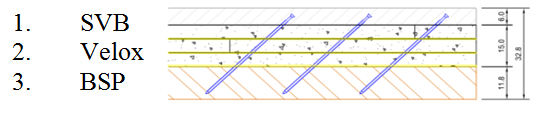
\includegraphics[scale =0.9]{Aufbau/bauteile/sandwich.png}
\caption{Sandwichaufbau}
\label{sandwichaufbau}
\end{center}
\end{figure}



\subsection{Verwendete Bauteilkomponenten}
\subsubsection{Selbstverdichtender Beton, SVB}

Selbstverdichtender Beton ist ein besonders fließfähiger Beton, der sich selbst entlüftet und eine ebene Oberfläche bildet. Durch die Fließfähigkeit ist ein besonders guter Verbund mit dem porösem Werkstoff Holzbeton (Velox) gewährleistet. Die Betonschicht wurde auf eine minimale Dicke von \unit[6]{cm} reduziert. Das Limit ergibt sich aus der Verankerungslänge der Schrauben (\unit[4]{cm}) zuzüglich einer Betondeckung von \unit[2]{cm}. Die Betonrezeptur hat Kirchmayer [] ausgearbeitet.


\begin{figure}[h]
\begin{center}
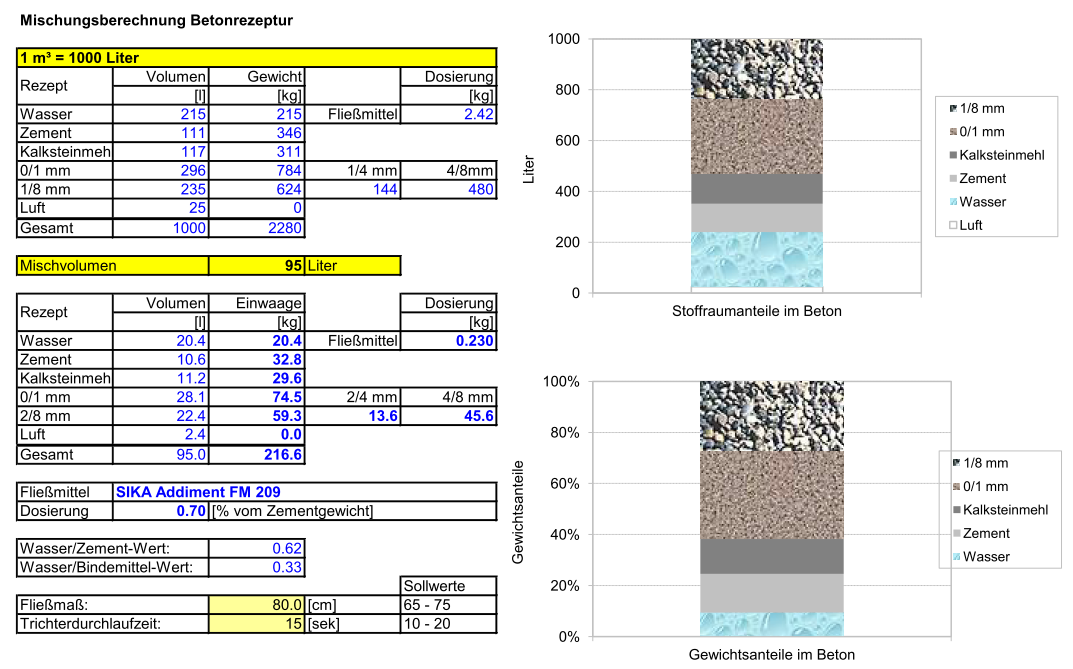
\includegraphics[scale =1.1]{Aufbau/bauteile/Beton-Mischrezeptur.png}
\caption{Beton-Mischrezeptur [2], mit Okamurarechner}
\label{Beton-Mischrezeptur}
\end{center}
\end{figure}


\subsubsection{Holzspanbeton/ Holzleichtbeton}

Holzspanbeton besteht aus den Komponenten Zement, Sägespänen, Wasser, Additiven und Zuschlagstoffen. Die Auswahl des Materials geht auf die Vorversuche von Kirchmayer bzw. Schernberger zurück. 
Die Abmessungen der Holzbetonschicht ergab sich aus einem Vielfachen der Dicke der Velox-Platten (\unit[50]{mm}) und aus Vorberechnungen mit den FEM-Programm        "`Sofistik"'. Die Veloxplatte ist ein Industrieprodukt, das ausführlich in der Ausarbeitung von Kirchmayer beschrieben wird.


\begin{figure}[h]
\begin{center}
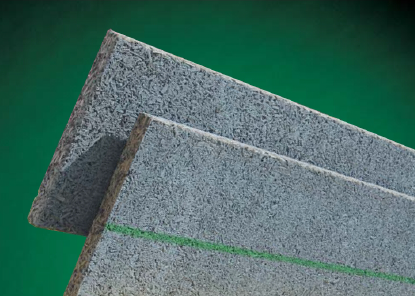
\includegraphics[scale =0.7]{Aufbau/bauteile/velox.png}
\caption{Holzspanplatte WS 50 der Firma Velox}
\label{velox}
\end{center}
\end{figure}

\subsubsection{Brettsperrholz, BSP}

Die Brettsperrholzplatte ist ein flächiges Holzprodukt aus mindestens drei rechtwinkelig zueinander verleimten Schichten. BSP wird im Holzmassivbau eingesetzt und kann mit großen Abmessungen hergestellt werden. Es wurde auch schon in den Vorversuchen von Kirchmayer angewendet. Die Vorteile hat ebenfalls  Kirchmayer [] schon ausgearbeitet.

Es wurde für alle Bauteilversuche das Produkt BSP 118 3s DL ind. verwendet. In Abbildung \ref{clt} ist ein Beispielbild einer fünf-schichtigen BSP-Platte dargestellt.

\begin{figure}[h]
\begin{center}
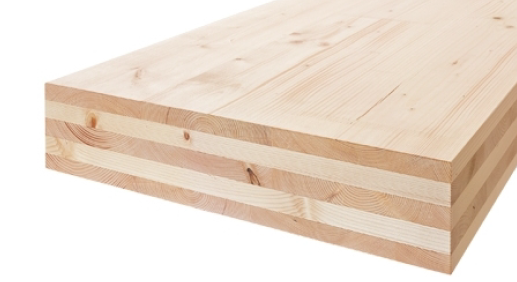
\includegraphics[scale =0.7]{Aufbau/bauteile/clt.png}
\caption{fünfschichtige Brettsperrholzplatte (BSP der Fa. Mayr-Melnhof)}
\label{clt}
\end{center}
\end{figure}

\subsubsection{Verbindungsmittel}

Um einen kraftschlüssigen Verbund der einzelnen Bauelemente herstellen zu können, kamen verschiedene Verbindungsmittel zur Anwendung. Aus den Vorversuchen von Kirchmayer ist hervorgegangen, dass die besten Verbundergebnisse durch Schrauben und Kleber  erzielt worden sind. Dieser Ansatz wurde weiter verfolgt.




\begin{itemize}
\item Schrauben
\newline
Die verwendeten Schrauben sind durch die Versuche ( Siehe Kapitel\,2) ausgewählt worden.
\newline
\begin{itemize}
\item SFS Intec WR-T-9x400
\end{itemize}

\item Kleber

Die angeführten Kleber sind im Kapitel 2 beschrieben.
\newline

\begin{itemize}
\item Sikadur-31 AUT Normal
\item SikaTop-109 ElastoCem 
\item Sikatop-107 Seal
\end{itemize}

\end{itemize}

\subsection{Herstellung des Sandwichaufbaus}
Der Zweikomponenten-Kleber wurde mit dem Mischverhältnis, das vom Hersteller angegeben wird, abgemischt. Die erste Kleberschicht wurde auf die BSP-Platte aufgetragen. Das Auftragen erfolgte mit einer  \unit[8]{mm} Zahnspachtel. Für die Verarbeitungszeit des Klebers war laut Datenblatt \unit[45]{min} Topfzeit vorgegeben. Auf die Kleberschicht wurden die Velox-Platten aufgelegt. Dieser Schritt wurde drei mal wiederholt. 

\begin{figure}[h!]
	\begin{minipage}[h]{7cm}	
	 	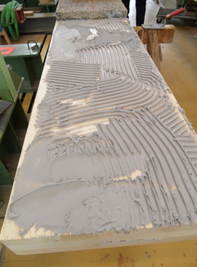
\includegraphics[width=7cm]{Aufbau/herstellung/kleberauftrag.png}
		\caption{Kleberauftrag auf die BSP-Platte}
		\label{kleberauftrag}
	\end{minipage}
		\hfill
	\begin{minipage}[h]{7cm}
		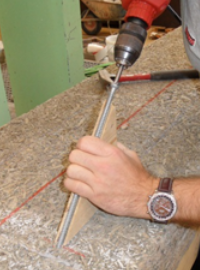
\includegraphics[width=7cm]{Aufbau/herstellung/einschrauben.png}
		\caption{Einschrauben der Schrauben}
		\label{einschrauben}
	\end{minipage}
\end{figure}




Im nächsten Schritt wurde das Bohrmuster auf der obersten Velox-Platte aufgezeichnet. Die Schrauben wurden mit einem Hilfswinkel (Holzstück) und einem Hammer angesetzt um den Einschraubwinkel   (\unit[45]{$^{\circ}$}) einzuhalten. Die Schrauben wurden anschließend ohne Vorbohren mit einer Bohrmaschine in den Bauteil eingebohrt, bis die Schrauben nur noch \unit[4]{cm} aus der oberen Velox-Schicht herausstanden. 
	

Der letzte Schritt vor dem Betonieren war das Anbringen der Schalung. Es wurden Schalungsbretter auf eine Höhe von \unit[20]{cm} zugeschnitten. Die Schalung wurde mit einem Überstand von \unit[6]{cm} über der letzten Veloxschicht angebracht. Damit man den Überstand allseitig gleich hält, wurden zwei Holzstücke mit den geforderten \unit[6]{cm} gefertigt. Somit hatte sich das Einrichten der Bretter einfach gestaltet.  Die Bretter wurden an die Velox-Schicht angeschraubt .


Abschließend wurde der Beton hergestellt. Die einzelnen Bestandteile wurden nach der Betonrezeptur [Abbildung: \ref{Beton-Mischrezeptur}] exakt eingewogen und mit einem Zwangsmischer vermischt. Der Beton wurde von Hand aufgebracht. Zum Schluss wurde der Beton mit einer Latte abgezogen und mit einem Schwert geglättet.


	



\begin{figure}[h!]
\begin{minipage}[h]{7cm}	
	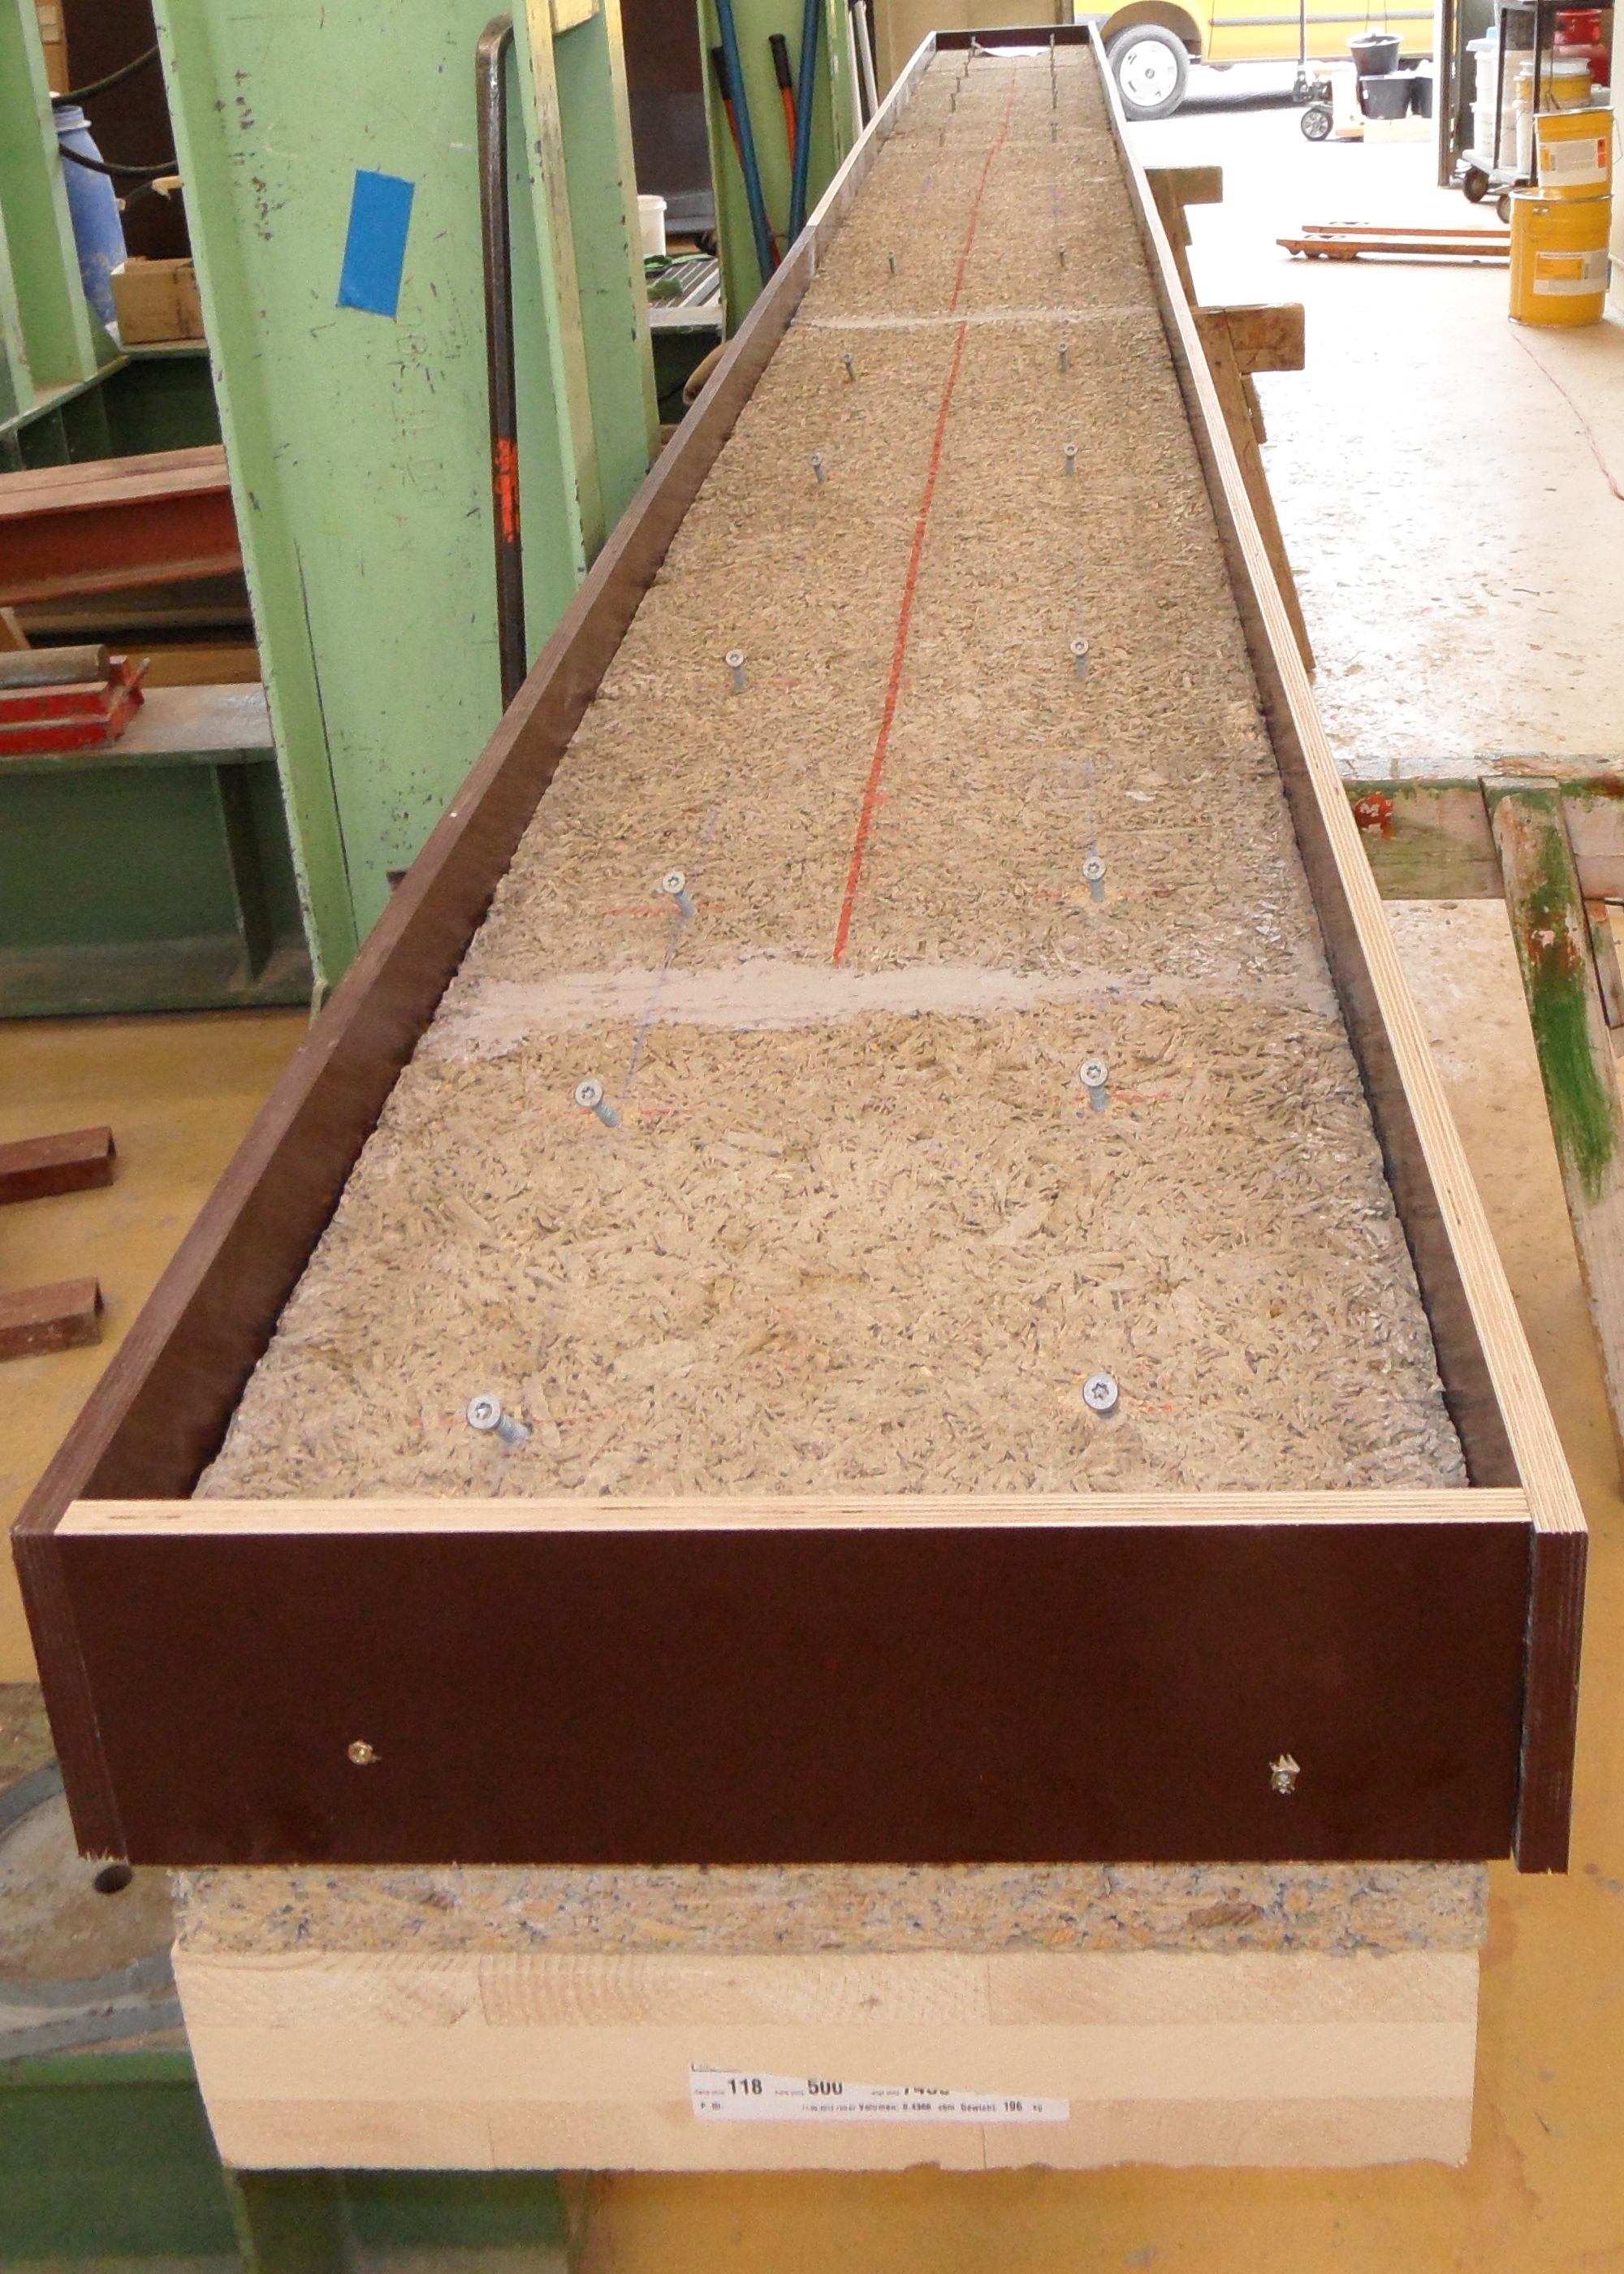
\includegraphics[width=7cm]{Aufbau/herstellung/einschalen.png}
	\caption{Befestigung der Schalung am Velox}
	\label{einschalen}
	
\end{minipage}
\hfill
\begin{minipage}[h]{7cm}
	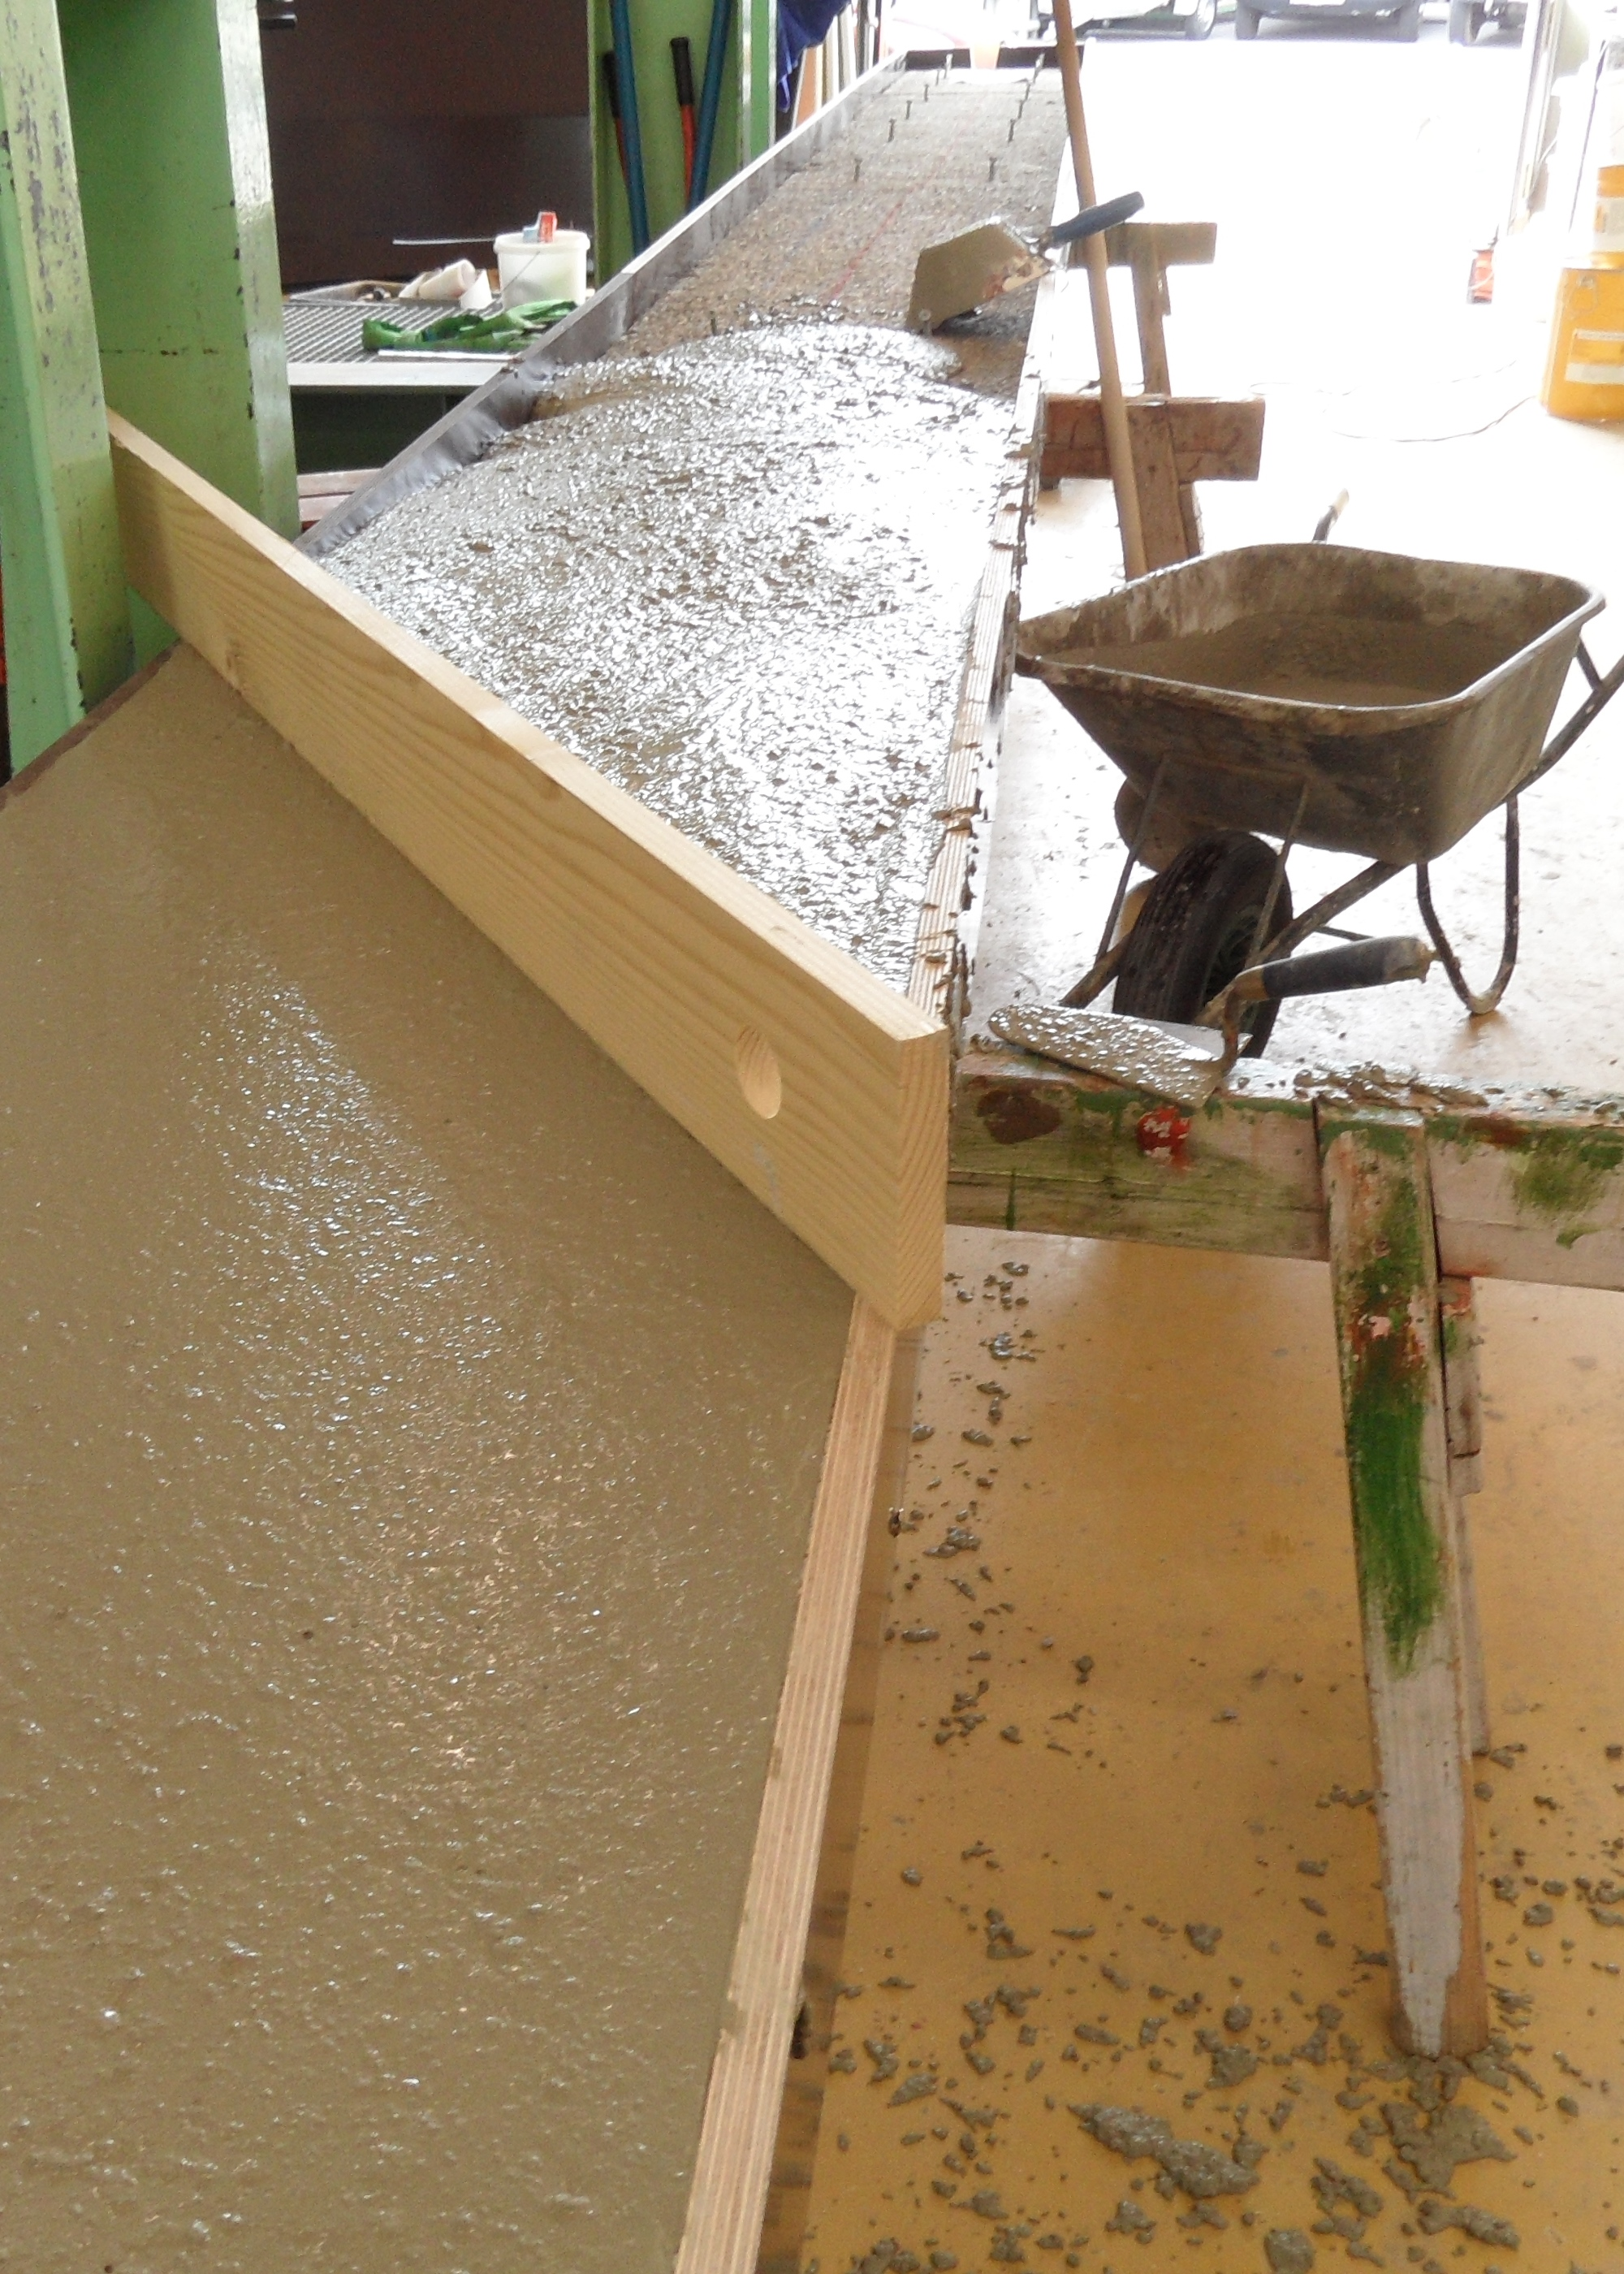
\includegraphics[width=7cm]{Aufbau/herstellung/betonieren.png}
	\caption{Einbrinden und Abziehen des SVB}
	\label{betonieren}
\end{minipage}
\end{figure}



\subsection{Versuchsaufbau und Durchführung}
\label{abs:Versuchsbaufaufbau_Durchführung}
Die Abbildung \ref{versuchsaufbau} zeigt die Versuchsanordnung. Es handelt sich um einen 4-Punkt-Biegeversuch.   
Dabei wird die Prüfprobe auf zwei Auflagen (rote Dreiecke) positioniert und in den Viertel-Punkten mit der Kraft (\unit[F]) belastet. Die Momentenlinie ist zwischen den Krafteinleitungspunkten konstant und stellt eine Umhüllende, des parabelförmigen Momentenverlaufs, einer äquivalenten Flächenlast dar.

\begin{figure}[h]
\begin{center}
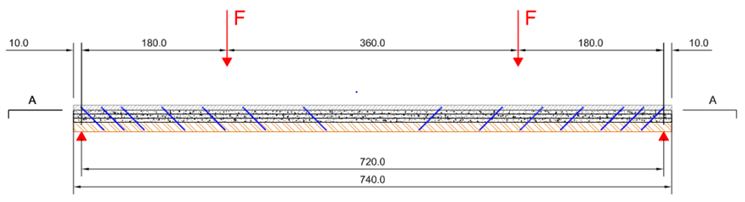
\includegraphics[scale =0.8]{Versuchsaufbau/versuchsaufbau.png}
\caption{Versuchsaufbau mit Lagerung und Lasteinleitung}
\label{versuchsaufbau}
\end{center}
\end{figure}

\subsubsection{Verwendete Messmittel und deren Anordnung}

 Die Wegaufnehmer für die Trägerdurchbiegung wurden in der Trägermitte und unter der Lasteinleitung angeordnet. Weiters wurde auf beiden Trägerenden Wegaufnehmer angebracht, um die Verschiebung zwischen Betonschicht und der BSP-Schicht zu messen. Bei dem ersten und zweiten Großbauteilversuch wurde die Verschiebung noch manuell von den Messuhren abgelesen. Bei den Bauteilversuchen 3 und 4 wurden  digitale Wegaufnehmer verwendet, die anschließend beschrieben werden. 
In der Abbildung \ref{versuchsaufbau} sind die Messpunkte skizziert und beschriftet.

\begin{figure}[h!]
\begin{center}
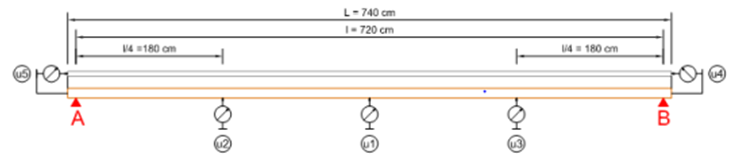
\includegraphics[scale =0.8]{Versuchsaufbau/messanordnung.png}
\caption{Anordnung der Messpunkte beim Bauteilversuch}
\label{versuchsaufbau}
\end{center}
\end{figure}


\begin{figure}[h!]
\begin{center}
	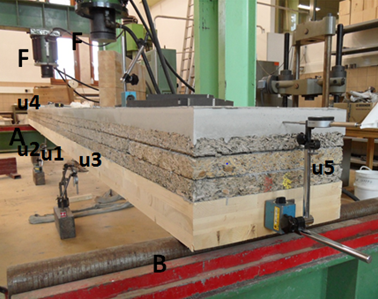
\includegraphics[scale=1.3]{Versuchsaufbau/messpunkte.png}
	\caption{Mess-und Auflagerpunkte beim Bauteilversuch}
	\label{messpunkte}
\end{center}
\end{figure}

	\begin{itemize}
	\item u1.1/ u1.2: Durchbiegung in Feldmitte 	auf beiden Seiten des Trägers
	\item u2/u3: Durchbiegung bei l/4
	\item u4/u5: Verschiebung der Betonschicht 	gegenüber der Holzschicht an beiden 	Enden des Trägers
	\item  Krafteinleitung F bei l/4
	\item A/B: Auflager
	\end{itemize}





\subsubsection{Wegaufnehmer}	

In diesem Abschnitt werden die die verschiedenen Wegaufnehmer beschrieben.

\paragraph{Anologe Wegaufnehmer}

Es wurden analoge Messuhren der Fa. Käfer verwendet. Die Messuhren haben einen Messweg von \unit[7]{cm} und  eine Messgenauigkeit von  \unit[1/100]{mm}.  Auf einen Standfuss wurden die magnetischen Halteeinrichtungen angebracht, welche die Messuhren in der vorgesehenen Position hielten. Der gesamte Aufbau ist in Abbildung \ref{messuhr_unten} dargestellt.

Die Befestigung für die horizontale Verschiebung wurde ebenfalls mit der magnetischen Halteeinrichtung bewerkstelligt. Zuvor musste noch eine Stahlplatte an der BSP-Platte angeschraubt werden, damit die Halteeinrichtung angebracht werden konnte. Der gesamte Aufbau kann Abbildung \ref{messuhr_seitlich} entnommen werden.

\begin{figure}
\begin{minipage}[h]{7cm}
	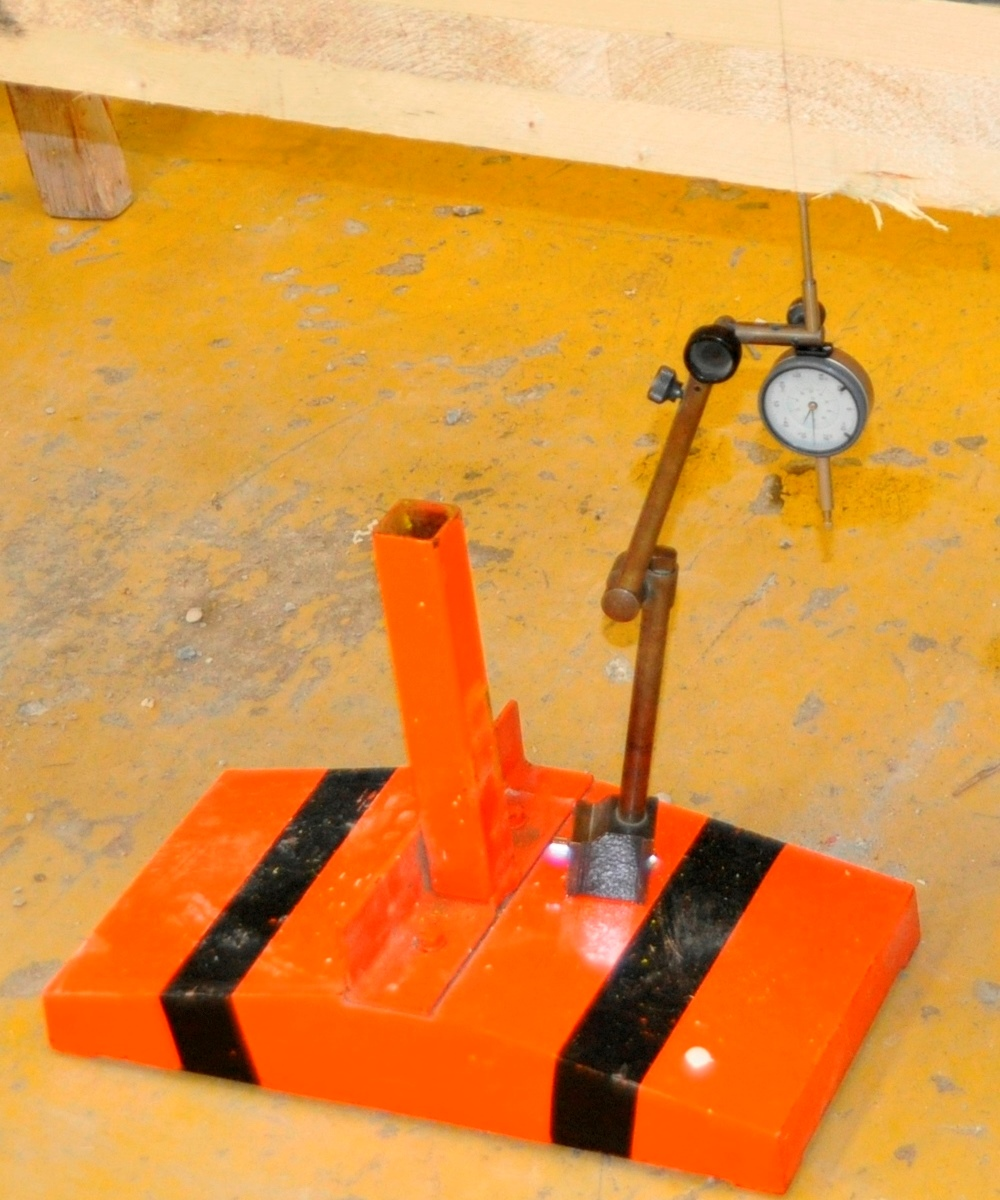
\includegraphics[width=7cm]{Versuchsaufbau/messuhr_unten.jpg}
	\caption{Messuhr für vertikale Verschiebung, befestigt am Standbein}
	\label{messuhr_unten}
\end{minipage}
\hfill
\begin{minipage}[h]{7cm}
	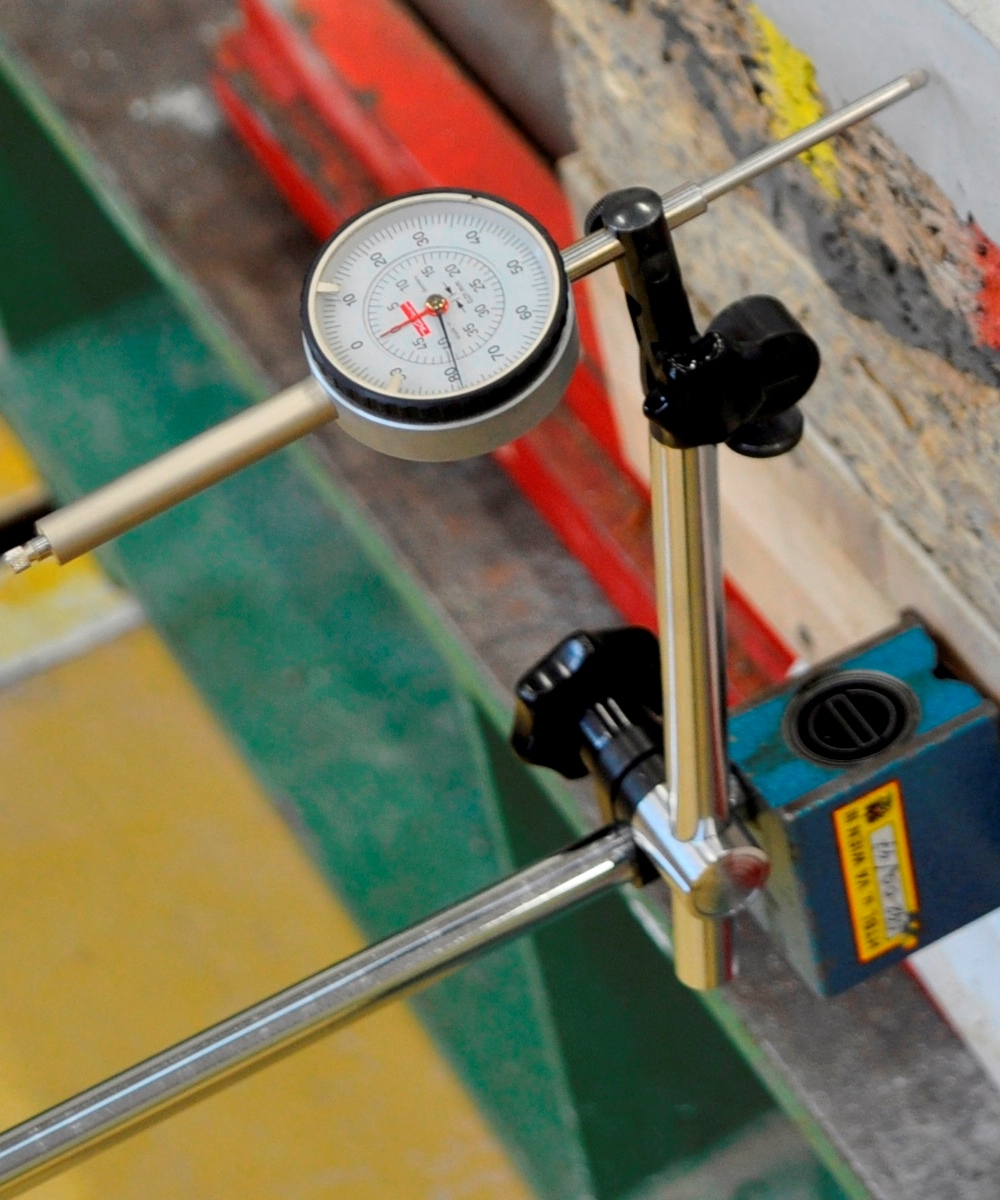
\includegraphics[width=7cm]{Versuchsaufbau/messuhr_seitlich.jpg}
	\caption{Messuhr für horizontale Verschiebung am Bauteilende}
	\label{messuhr_seitlich}
\end{minipage}
\end{figure}


\paragraph{Digitale Wegaufnehmer}

Es wurden digitale Seilzug-Wegsensoren der Fa. MICRO-EPSILON verwendet[Serie WDS, Baureihe P60, \unit[1000]{mm}]. Die Messuhren besaßen einen maximalen Messweg von \unit[100]{cm} und haben eine Messgenauigkeit von \unit[0,24]{mm}. Die Haltevorrichtung für die vertikale Verschiebung, wurde ebenfalls mit dem Standfuss ausgeführt. In den Standfuss wurde eine Metallstange eingeführt und mit kleinen Holzkeilen fixiert. Der  Wegsensor wurde mit M4 Schrauben, Flügelmuttern und einer Holzplatte an der Metallstange montiert. Das Seil wurde mit einer Holzschraube an der BSP-Platte befestigt. Der gesamte Aufbau ist in Abbildung \ref{d_aufnehmer_unten} dargestellt.

Für die Messung der horizontalen Verschiebung, wurde eine Haltevorrichtung herstellt. Die Vorrichung wurde mit Schrauben auf der BSP-Platte angeschraubt. Der Wegsensor wurden ebenfalls mit M4 Schrauben, Flügelmuttern und einer Holzplatte, an der Haltevorrichtung befestigt. Der gesamte Aufbau kann aus  Abbildung \ref{d_aufnehmer_seitlich} entnommen werden.



\begin{figure}[h!]
\begin{minipage}[h!]{7cm}
	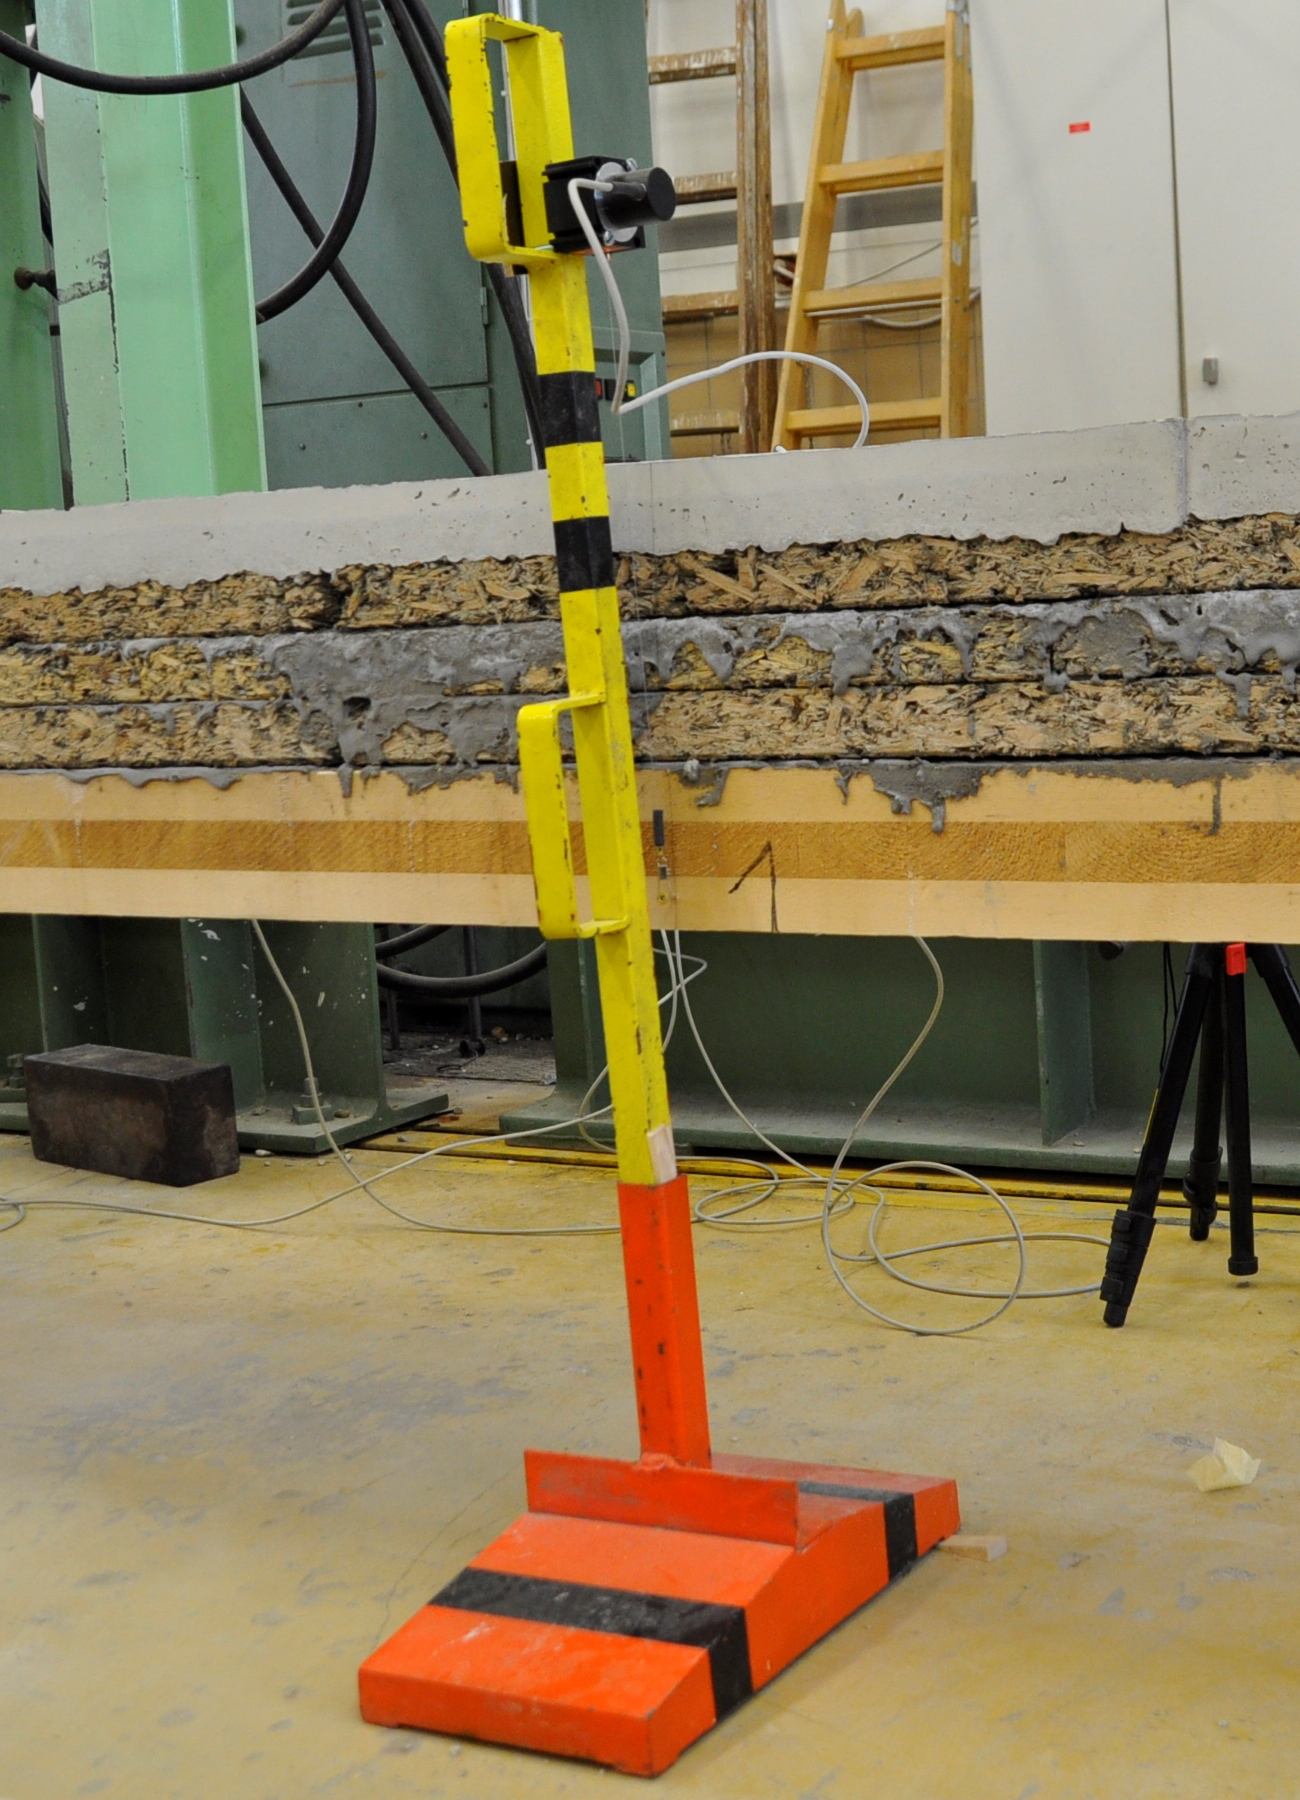
\includegraphics[width=7cm]{Versuchsaufbau/d_aufnehmer_unten.jpg}
	\caption{Wegaufnehmer für vertikale Verschiebung mit Standbein und Stange}
	\label{d_aufnehmer_unten}
\end{minipage}
\hfill
\begin{minipage}[h!]{7cm}
	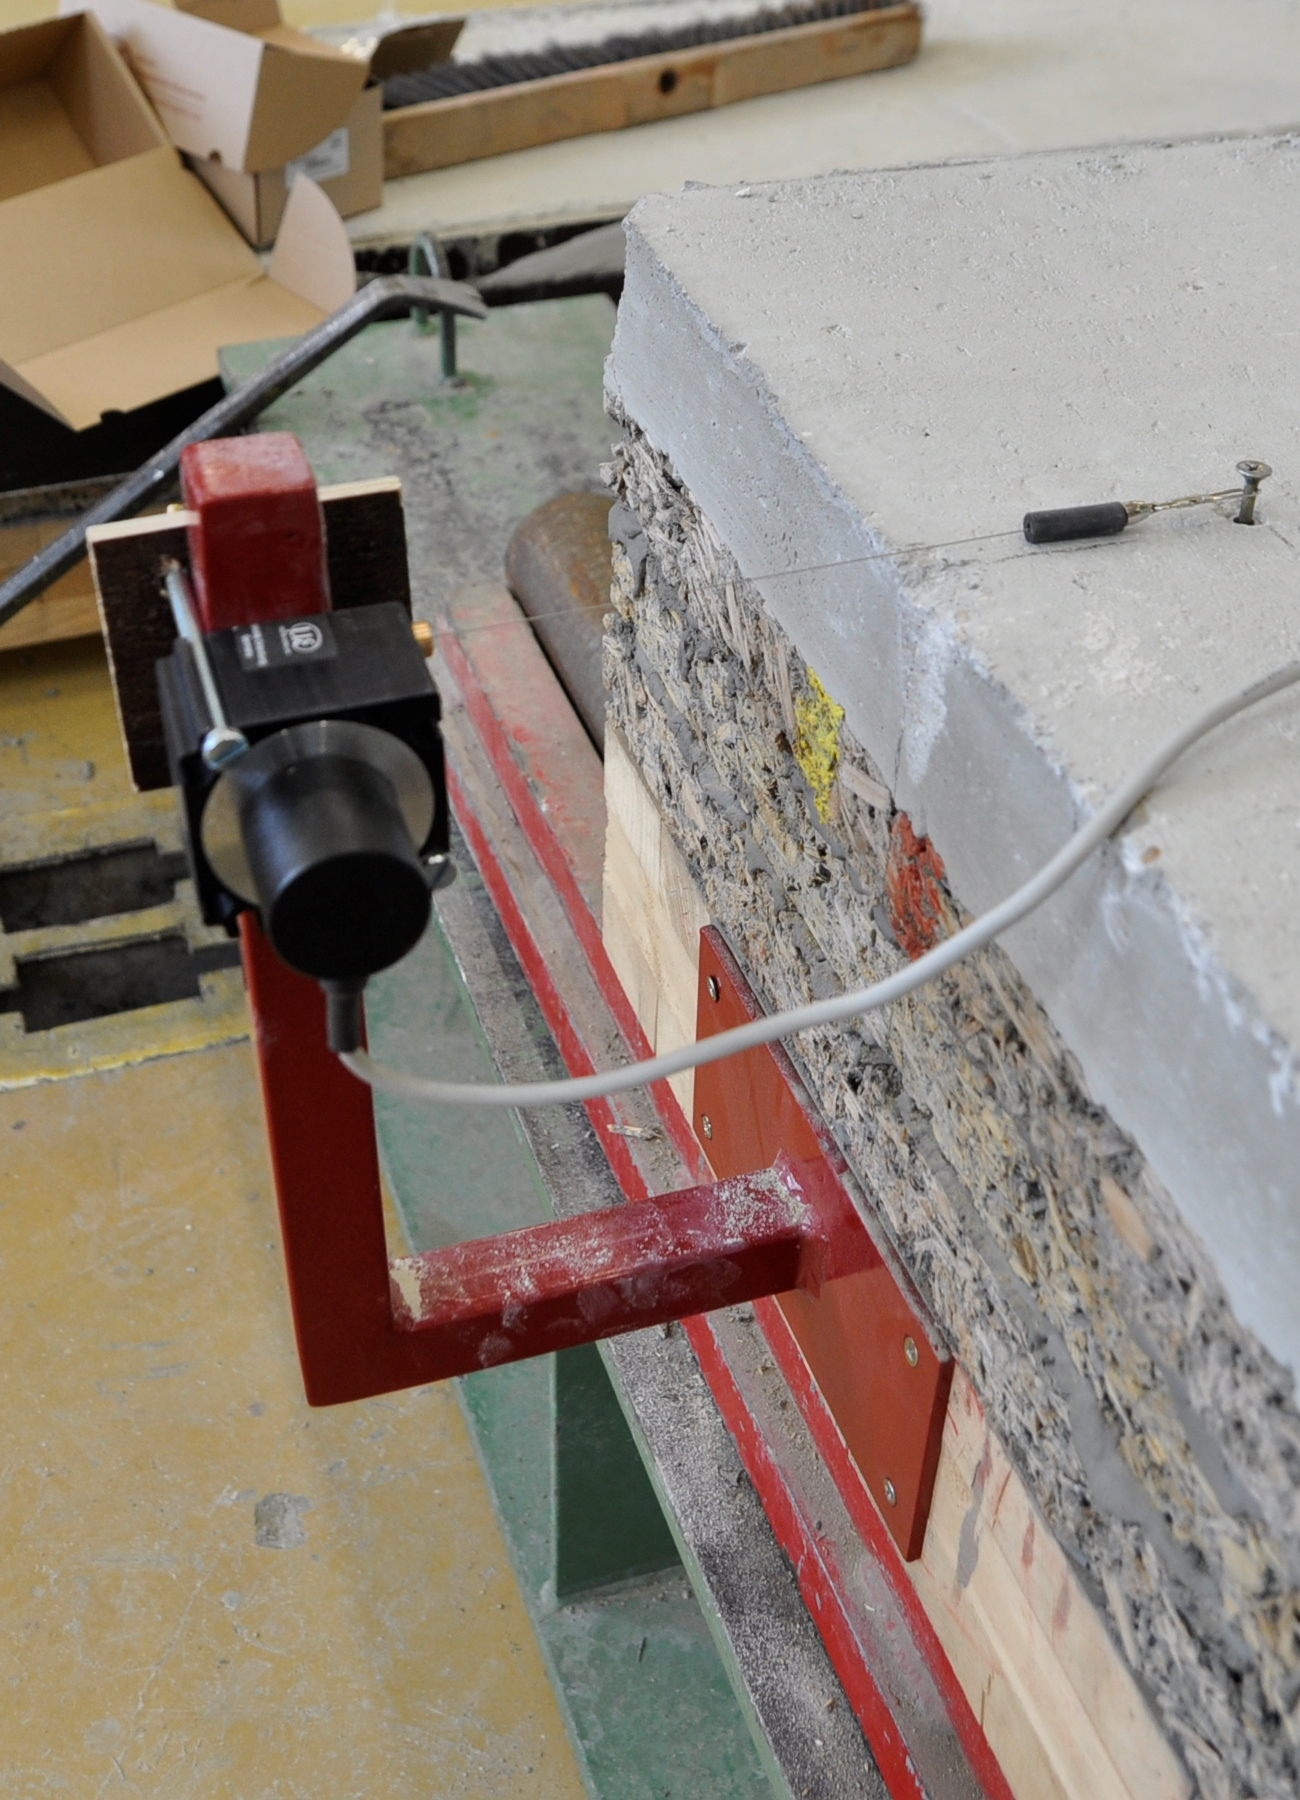
\includegraphics[width=7cm]{Versuchsaufbau/d_aufnehmer_seitlich.jpg}
	\caption{Wegaufnehmer für horizontale Verschiebung am Bauteilende}
	\label{d_aufnehmer_seitlich}
\end{minipage}
\end{figure}










	
\subsubsection{Durchführung des Versuchs}
Der Aufbau des Bauteilversuchs bzw. die Abmessungen des Bauteils ist  Abbildung \ref{versuchsaufbau} zu entnehmen. Für die Bauteilversuche 1 und 2 wurde eine Belastungsgeschwindigkeit von etwa \unit[4]{kN/min} gewählt. Das Ablesen erfolgte in Schritten von \unit[2]{kN}. Bei den Bauteilversuchen 3 und 4 wurde eine vorgegebene Belastungskurve gewählt. Die Kurve wurde der Norm [ÖN EN 380] entnommen. Das Grundverfahren der Belastung besteht aus den 7 Verfahrensstufen. 

\paragraph{Belastungserklärung}
\begin{itemize}
\item $G_{1}$\ldots Eigengewicht des Bauteils
\item $G_{2}$\ldots Gewicht des erforderlichen Aufbaus (Dämmung, Estrich, Bodenbelag)
\item $Q$ \ldots veränderliche Last lt. EC1 für Wohnräume
\item Belastungsgeschwindigkeit: \unit[1,5]{kN/min}
\item Die Lastangaben beziehen sich auf einen Zylinder.
\end{itemize}
	

\begin{figure}
\begin{center}

	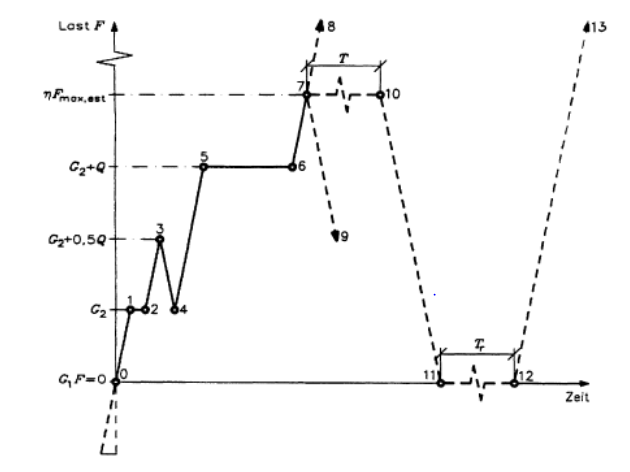
\includegraphics[width=12cm]{Versuchsaufbau/belastungskurve.png}
	\caption{Schematische Belasungskurve, nach []}
	\label{belastungskurve}

\end{center}	
\end{figure}	

\begin{table}
\caption{Grundlagen der Belastung,[]}
\begin{center}
\begin{tabular}{|c|c|c|c|}
\hline 
Verfahrensstufe & Belastungsverfahren & Zeit in [s] & F [kN] \\ 
\hline \hline
0 & Es wirkt nur G;F=0 &  &  \\ 
\hline 
0-1 & F=G aufbringen &  & 2,70 \\ 
\hline 
1-2 & F=G konstant halten & 120 & 2,70 \\ 
\hline 
2-3 & F=G+0,5*Q aufbringen & 120 & 5,40 \\ 
\hline 
3-4 & 0,5 Q entlasten & 120 & 2,70 \\ 
\hline 
4-5 & F=G+Q aufbringen & 240 & 8,10 \\ 
\hline 
5-6 & F=G+Q konstant halten & 600 & 8,10 \\ 
\hline 
6-8 & F= steigern bis Bruch &  &  \\ 
\hline \hline
\multicolumn{4}{|c|}{ max. Belastungsgeschwindigkeit 0,25Q je 60 sec} \\ 
\hline 
\end{tabular} 
\label{tab:belastung}
\end{center}
\end{table}


\section{Bauteilversuche}

\subsection{Allgemeines}

Die Tabelle \ref{tab:Versuchsprogramm} gibt einen Überblick über die Bauteilversuche  und die Unterschiede im Aufbau. Grundlage für die Änderungen der Bauteilkomponenten waren der Gedanke die Material- und Herstellungskosten zu reduzieren. 

\begin{table}[h]
\caption{Versuchsprogramm}
\begin{center}
\begin{tabular}{|c|c|c|c|c|}
\hline 
\multicolumn{5}{|c|}{ Übersicht} \\ 
\hline 
Versuch & Abmessungen  & Schraubenanzahl & Kleber & Aushärtezeit \\ 

&  l x b x h in [m] & (Fa. SFS) & (Fa. Sika)   & Tage \\ 
\hline\hline
1 & 7,40 x 0,50 x 0,33 & 28 & Sikadur 31   & 14 \\ 
\hline 
2  & 7,40 x 0,50 x 0,33 & 8 & ElastoCem 109  & 21 \\ 
\hline 
3 & 7,40 x 0,50 x 0,33 & 12 & Sikatop 107  & 28 \\ 
\hline 
4  & 7,40 x 0,50 x 0,33 & - & Sikatop 107  & 28 \\ 
\hline 
\end{tabular} 
\end{center}
\label{tab:Versuchsprogramm}
\end{table}

\subsection{Bauteilversuch\,1\,(BT\,1)}

\subsubsection{Versuchskörper}

Der grundsätzliche Schichtenaufbau ist in Abschnitt 2.1.2 beschrieben. 

 Die Anordnung der Schrauben ist der Abbildung \ref{1versuch} zu entnehmen. Die Schrauben wurden analog zum Verlauf der Querkraftlinie zufolge einer Gleichlast angeordnet, d.h.\ im Auflagerbereich ist der Schraubenabstand geringer als in Trägermitte. Es wurde zwischen der Holz und Holzbetonschicht sowie zwischen den Holzbetonschichten der Kleber SikaDur 31-A Normal verwendet. 
 
  Die Durchbiegungen wurden an den Rändern des Trägers gemessen. 
Um eine auftretende Torsion während des Versuchs erfassen zu können, wurden in der Trägermitte zwei Messuhren an den Ränders angebracht.


\begin{figure}[h!]
\begin{center}
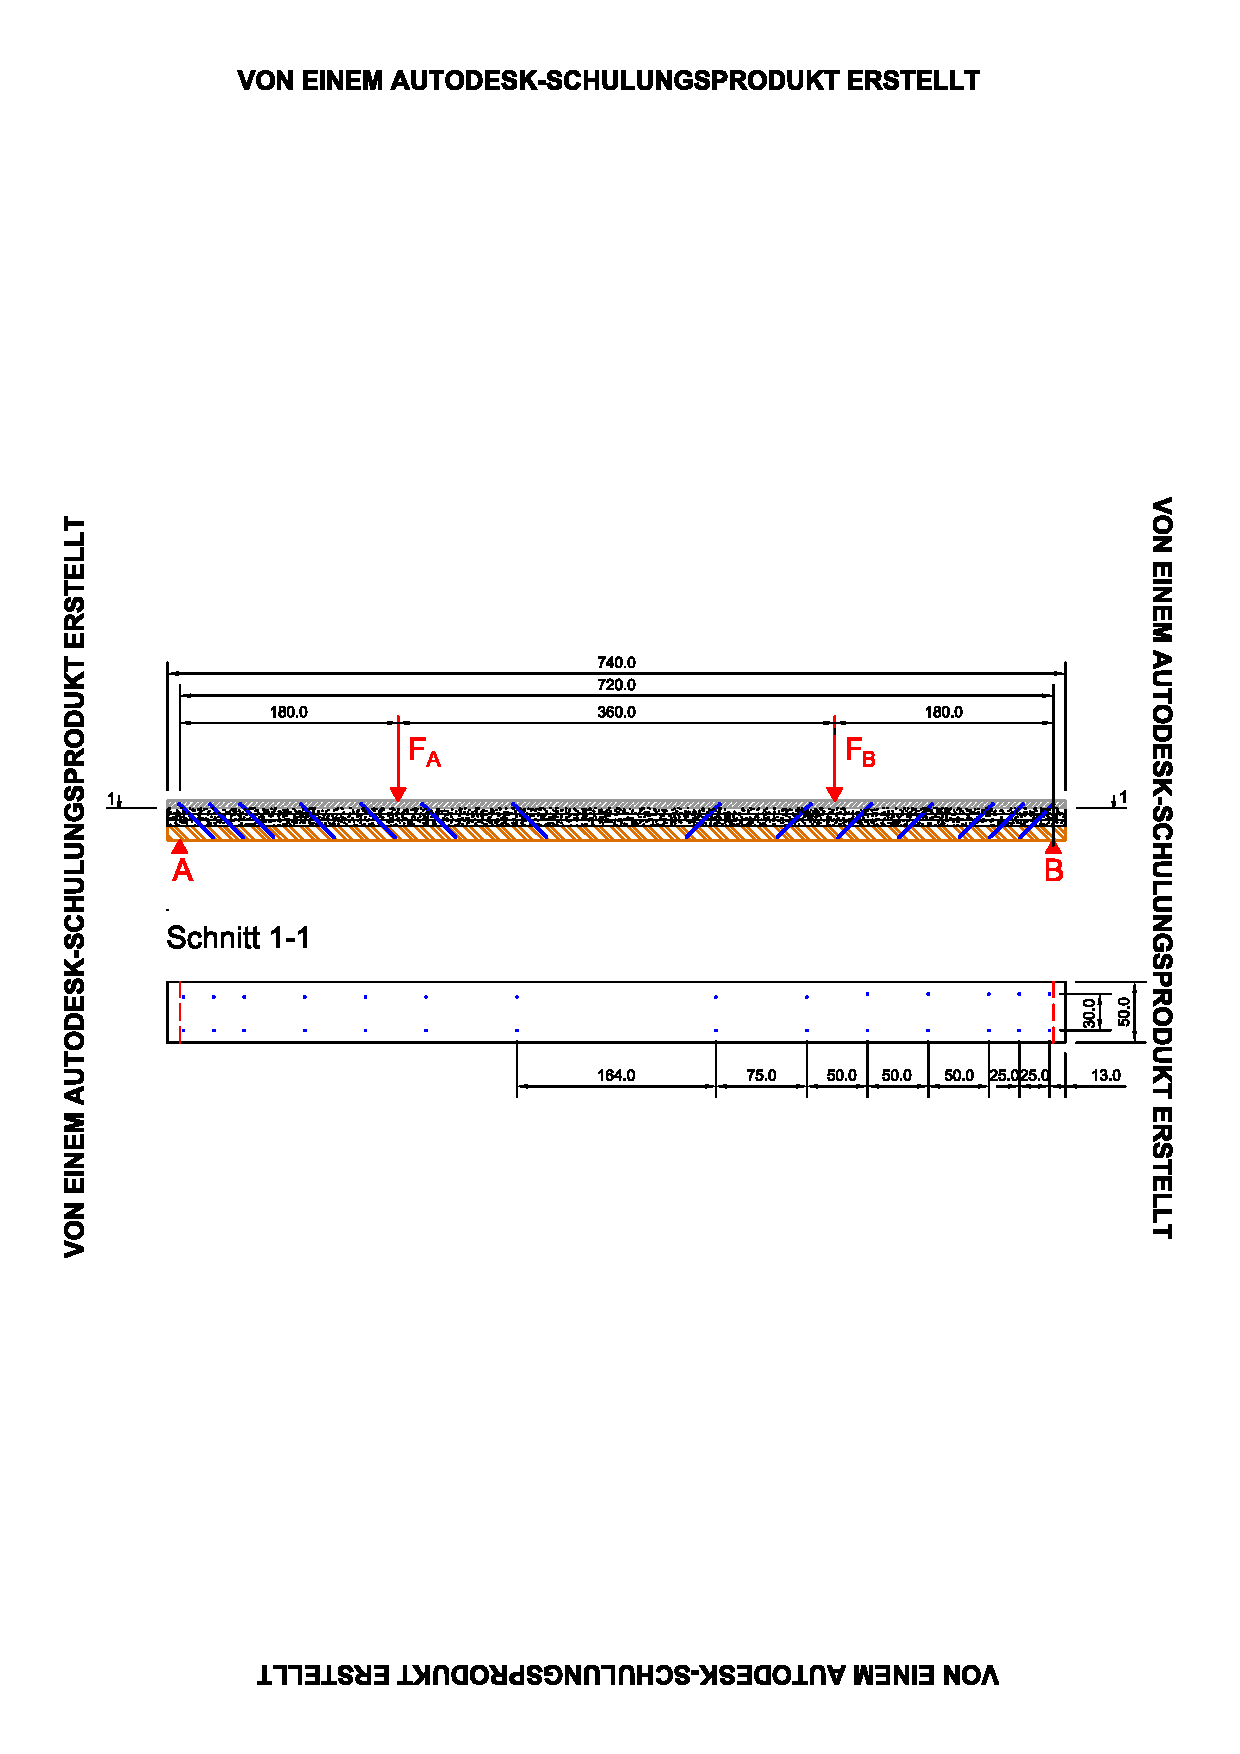
\includegraphics[scale =0.9,trim= 1.5cm 10cm 1.5cm 10cm, clip=true]{Auswertung/1versuch/BT1.pdf}
\caption{Darstellung des BT\,1, mit Verbindungsmittel und Lasteinleiung}
\label{1versuch}
\end{center}
\end{figure}

\subsubsection{Versuchsablauf}

Der Versuch wurde manuell kraftgesteuert durchgeführt, die Belastungsgeschwindigkeit betrug etwa \unit[4]{kN/min}. Bei der Laststufe von \unit[58]{kN} (je Zylinder) wurde ein Haltepunkt eingefügt, da eine Keilzinkung versagte (Abbildung \ref{keilzinkung}). 

Bei weiterer Belastung wurde die Maximallast von \unit[78]{kN} erreicht. Nach dieser Laststufe erhöhte sich die Durchbiegung sprunghaft bei gleichzeitiger Reduktion der aufgebrachten Last.

Um einen vollständigen Bruch des Systems herbeizuführen, wurde der Bauteil nochmals belastet. Der Bruch trat bei einer Last von \unit[48]{kN} ein (Abbildung \ref{1bruch}).

\subsubsection{Versagensbeschreibung}

Das erste Versagen wurde bei einer Last von \unit[58]{kN} festgestellt. Unter $F_{A}$ brach eine Keilzinkung der Brettsperrholzplatte. In Abbildung \ref{keilzinkung} ist der Schaden am Bauteil darstellt. Im Diagramm in Abbildung \ref{1_versuch_kraft_schubverschiebung} ist zu erkennen, dass vor dem erreichen dieser Laststufe bereits eine erhöhte horizontale Verschiebung zwischen Beton und Holz bei Auflager A stattfand. 

Das Versagen der Klebefuge führte zu einer Spannungsumlagerung in den Teilquerschnitten Beton und Holz. 
Durch die aus der Spannungsumlagerung erhöhten Randspannungen brach die Keilzinkung unter dem Lasteinleitungspunkt $F_{A}$(Abbildung \ref{keilzinkung}).  
  
Beim weiteren Belasten waren Risse im Beton zwischen der Kraft $F_{A}$ und dem Auflager A entstanden. Die maximale Belastung betrug \unit[78]{kN}. 



Durch den Bruch konnte danach die Fuge zwischen Holzspanbeton und Holz betrachtet werden (Abbildung \ref{bruchbild}). Es zeigte sich, dass ca.\ ein Viertel der Fläche ungenügenden Verbund hatte. Ein Grund für das Versagen der Verbundfuge dürfte in der ungenügenden Vernetzung der Klebeschicht zwischen Holz und Holzbeton liegen. Durch den unzureichenden Verbund kam es zu höheren Biegespannungen in den Teilquerschnitten Holz und Beton und damit zum Bruch der Keilzinkung.

Desweiteren wurde ersichtlich, dass in diesem Bereich des Trägers zwei Schrauben nicht aus dem Holz ausgezogen wurden, sondern in der Klebefuge zwischen Holz und Holzbeton abgerissen sind. Die restlichen Schrauben wurden aus der Brettsperrholzplatte ausgezogen. 




\begin{figure}[h!]
\begin{minipage}[hbt]{7cm}
	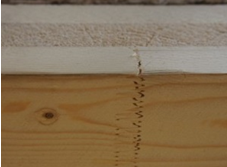
\includegraphics[width=7cm]{Auswertung/1versuch/keilzinkung.png}
	\caption{Versagen der Keilzinkung unter der Lasteinleitung $F_{A}$ }
	\label{keilzinkung}
\end{minipage}
\hfill
\begin{minipage}[hbt]{7cm}
	\includegraphics[width=7cm]{Auswertung/1versuch/Betonriss78kN.jpg}
	\caption{Betonriss im Bereich der Krafteinleitung $F_{A}$ nach Maximalbelastung }
	\label{1bruch}
\end{minipage}
\end{figure}
 


\begin{figure}[h!]
\begin{minipage}[hbt]{7cm}
	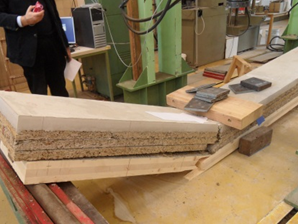
\includegraphics[width=7cm]{Auswertung/1versuch/bruch_1versuch.png}
	\caption{Bruch nach Wiederbelastung }
	\label{1bruch}
\end{minipage}
\hfill
\begin{minipage}[hbt]{7cm}
	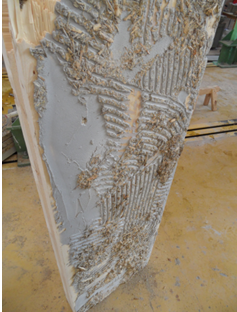
\includegraphics[width=7cm]{Auswertung/1versuch/bruchbild.png}
\caption{Bruchbild der BSP-Platte }
	\label{bruchbild}
\end{minipage}
\end{figure}

\subsubsection{Verformungsverhalten}

In Abbildung \ref{1 Versuch: Kraft-Durchbiegung} ist die Arbeitslinie des Versuchs dargestellt.

Sie weist einen annähernd linearen Verlauf bis zu der Kraft von \unit[58]{kN} auf. Wie im Diagramm ersichtlich, besteht kein Unterschied zwischen den Messpunkten  u\,1.1 und u\,1.2, d.h.\ es kam zu keiner Torsion während des Versuch.
Der weitere Verlauf der Kennlinie ist mit einigen Knicken versehen, die als Datenerfassungsfehler interpretiert werden. 

Abbildung \ref{1_versuch_kraft_schubverschiebung} zeigt die relative Verschiebung zwischen der BSP-Schicht und der Betonschicht. Bis zur Laststufe von \unit[35]{kN} trat keine messbare Verschiebung auf. Weiters ist erkennbar, dass bei \unit[58]{kN} der Verbund zwischen der BSP-Schicht und der Holzbetonschicht nicht mehr vorhanden war. 

Die Abflachung der Kurve zwischen \unit[58] und \unit[60]{kN} beinhaltet die Kriechverformung zufolge der konstant gehaltenen Kraft von \unit[58]{kN}(siehe auch Abbildung \ref{1 Versuch: Kraft-Durchbiegung-Zeit}). Während die Kurve u\,4 (Verschiebung bei Auflager B) bei weiterer Belastung die gleiche Steigung wie vor dem Haltepunkt aufweist, zeigt die Kurve u\,5 das fortschreitende Versagen der Schubverbindungen zwischen Beton und Holz. 


\begin{figure}[h!]
\begin{center}
\begin{tikzpicture}
\begin{axis}[height=12cm, width=12cm, 
			no markers,
			xmajorgrids,ymajorgrids,
			ylabel=Kraft\,/\,Zylinder\,$\lbrack kN\rbrack$,
			xlabel=Verschiebung\,u\,$\lbrack mm\rbrack$,
			xmin=0,ymin=0,
			legend pos=south east			
			 ]
\addplot table[y=F,x=u1.1]{Auswertung/1versuch/BT1.dat};
\addplot table[y=F,x=u1.2]{Auswertung/1versuch/BT1.dat};
\addplot table[y=F,x=u2]{Auswertung/1versuch/BT1.dat};
\addplot table[y=F,x=u3]{Auswertung/1versuch/BT1.dat};
\legend{BT1\,u1.1,BT1\,u1.2,BT1\,u2,BT1\,u3};
\end{axis}
\end{tikzpicture}
\caption{Bauteilversuch 1: Kraft-und Verschiebungsverlauf}
\label{1 Versuch: Kraft-Durchbiegung}
\end{center}
\end{figure}

\begin{figure}[h!]
\begin{center}
\begin{tikzpicture}
\begin{axis}[height=12cm, width=12cm,
			axis y line*=left, 
			no markers,
			xmajorgrids,ymajorgrids,
			xlabel=Zeit\,$\lbrack s \rbrack$,
			ylabel=Kraft\,/\,Zylinder\,$\lbrack kN\rbrack$,
			xmin=0,ymin=0,
			legend pos= north east			
			 ]
\addplot table[y=F,x=t]{Auswertung/1versuch/BT1.dat};
\legend{F};
\end{axis}
\begin{axis}[height=12cm, width=12cm, 
			axis y line*=right,
			axis x line*=none,
			no markers,
			xmajorgrids,ymajorgrids,
			ylabel=Verschiebung\,u\,$\lbrack mm\rbrack$,
			xmin=0,ymin=0,
			legend pos=south east			
			 ]
\addplot table[y=u1.1,x=t]{Auswertung/1versuch/BT1.dat};
\addplot table[y=u1.2,x=t]{Auswertung/1versuch/BT1.dat};
\addplot table[y=u2,x=t]{Auswertung/1versuch/BT1.dat};
\addplot table[y=u3,x=t]{Auswertung/1versuch/BT1.dat};
\legend{BT1\,u1.1,BT1\,u1.2,BT1\,u2,BT1\,u3};
\end{axis}
\end{tikzpicture}
\caption{Bauteilversuch 1: Kraft-und Verschiebungsverlauf in Abhängigkeit von der Zeit}
\label{1 Versuch: Kraft-Durchbiegung-Zeit}
\end{center}
\end{figure}




\begin{figure}[h!]
\begin{center}
\begin{tikzpicture}
\begin{axis}[height=12cm, width=12cm,
			no markers,
			xmajorgrids,ymajorgrids,
			xlabel=Verschiebung\,u\,$\lbrack mm \rbrack $,
			ylabel=Kraft\,/\,Zylinder\, $\lbrack kN \rbrack $,			
			xmin=0,ymin=0,
			legend pos= south east
			 ]
				\addplot table[y=F,x=u4]{Auswertung/1versuch/BT1.dat};
				\addplot table[y=F,x=u5]{Auswertung/1versuch/BT1.dat};
				\legend{BT1\,u4,BT1\,u5}
\end{axis}
\end{tikzpicture}
\caption{Bauteilversuch 1: Kraft-Schubverschiebung}
\label{1_versuch_kraft_schubverschiebung}
\end{center}
\end{figure}



\clearpage
 
\subsection{Bauteilversuch\,2\,(BT\,2)}

\subsubsection{Versuchskörper}

Der grundsätzliche Schichtenaufbau ist in Abschnitt 2.1.2 beschrieben.

Im Unterschied zum Versuch BT\,1 (ref) wurden die Schrauben analog zum Querkraftverlauf zufolge der  Belastungsanordnung im Versuch positioniert. Mittels einer Finite Elemente Berechnung mit dem Programm Sofistik wurde die Lage der Schrauben so optimiert, dass die Schrauben die gleiche Normalkraft erfahren. 



Nach den Kleberversuchreihe\,1(ref) wurde der Kleber ElastoCem 109 verwendet.


\paragraph{Schädigungen vor Versuchsdurchführung}
\label{abs:BT2_Schaden}

Die Schädigungen sind beim Einheben des Trägers in die Prüfanlage aufgetreten. Der Träger wurde mit zwei Gurten, die im einem Abstand von\unit[3]{m} zueinander in der Mitte des Trägers befestigt wurden, angehoben. Durch den daraus resultierenden Lastzustand entstanden die Betonzugrisse im Abstand von ca.\ \unit[150]{cm} von den Trägerenden (Abbildung \ref{schädigung scc}) und der Spalt in der obersten Klebefuge an den Trägerenden (Abbildung \ref{schädigung velox}).

Über die gesamte Länge des Träger wurden außerdem in der obersten Kleberfuge ungenügende Vernetzungen im Randbereich der einzelnen Veloxplatten festgestellt. An diesen Stellen war jeweils ein deutlicher Spalt zwischen den Veloxschichten zu sehen. 

Entgegen der Resultate der Kleberversuchsreihe\,1 erwiesen sich die Eigenschaften des hier verwendeten Kleber als ungeeignet für das Sandwichsystem. 



\subsubsection{Versuchsablauf}

Der Versuch wurde ebenfalls manuell kraftgesteuert durchgeführt. 
Die Belastungsgeschwindigkeit betrug etwa \unit[4]{kN/min}.  

Die Maximalkraft betrug \unit[31]{kN}. Danach fiel die Belastung auf \unit[18]{kN} ab, als der maximale Zylinderweg der Prüfanlage erreicht wurde.
Um einen vollständigen Bruch des Systems herbeizuführen, wurde der Bauteil nochmals belastet. Der Bruch trat bei einer Last von \unit[21]{kN} ein ).



\begin{figure}[h!]
\begin{center}
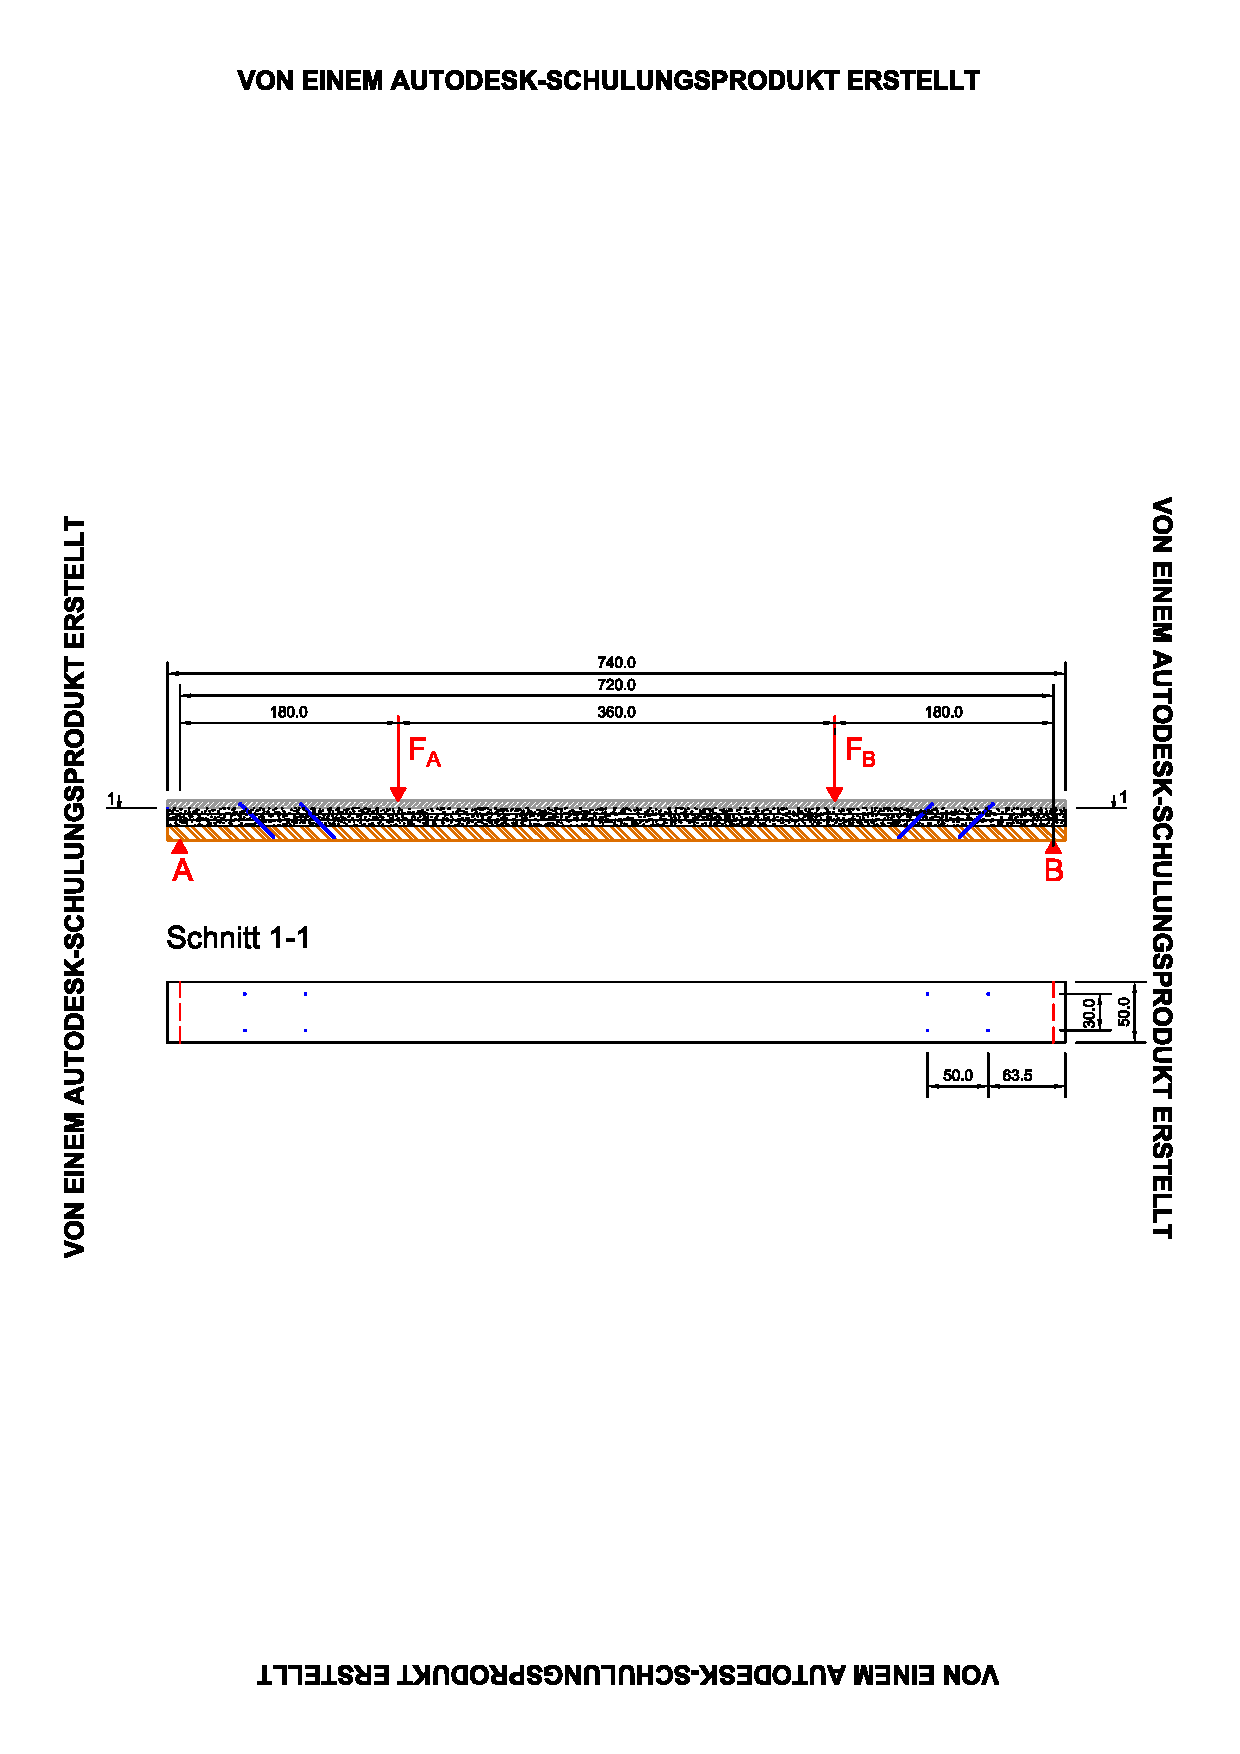
\includegraphics[scale =0.9,trim= 1.5cm 10cm 1.5cm 10cm, clip=true]{Auswertung/2versuch/BT2.pdf}
\caption{Darstellung des BT\,2, mit Verbindungsmittel und Lasteinleiung}
\label{1versuch}
\end{center}
\end{figure}



\begin{figure}[h]
\begin{minipage}[hbt]{7cm}	
	\includegraphics[width=7cm]{Auswertung/2versuch/schädigung_velox.jpg}
	\caption{Schädigung beim Auflager B}
	\label{schädigung velox}
\end{minipage}
\hfill
\begin{minipage}[hbt]{7cm}
	\includegraphics[width=7cm]{Auswertung/2versuch/schädigung_scc.jpg}
	\caption{Schädigung des Betons, bei $F_{B}$}
	\label{schädigung scc}
\end{minipage}
\end{figure}


\subsubsection{Versagensbeschreibung}

Abschnitt \ref{abs:BT2_Schaden} beschreibt die Schädigungen, die durch das Einheben des Trägers in die Prüfanlage entstanden sind.  

Wegen des großflächig nicht vorhandenen Verbundes in den Klebefugen (Abbildung \ref{velos unten} und \ref{velox ober}) wird davon ausgegangen, dass die mechanischen Verbindungsmittel (Schrauben) alleine die Verbundwirkung zwischen Holz und Beton herstellen. 

Bei der Laststufe von \unit[24]{kN} fand das erste sichtbare Versagen in der Holzschicht statt. Es spaltete sich ein Keil in der Zugzone in Trägermitte ab (Abbildung \ref{2versuch versagen}).

Bei der Maximallast von \unit[31]{kN} versagten die Schrauben beim Auflager A durch Herausziehen aus 
dem Holz. Es zeigt sich bei Betrachtung der überproportionalen Relativverschiebung zwischen Holz- und Betonschicht (Abbildung \ref{BT2_Verschiebung_AuflagerA} ). 
\subparagraph{Anmerkung:} Die Verschiebung ist im Diagramm in Abbildung \ref{2_versuch_kraft_schubverschiebung} nicht erfasst, da die analogen Wegaufnehmer aus Sicherheitsgründen zu diesem Zeitpunkt bereits entfernt worden sind. 

Der vollständige Bruch der BSP-Platte fand  nach Wiederbelastung zwischen dem Lasteinleitungspunkt $F_{A}$ und Trägermitte bei einer Last von \unit[21]{kN} statt (Abbildung \ref{2versuch bruchbild}).




\begin{figure}
\begin{center}
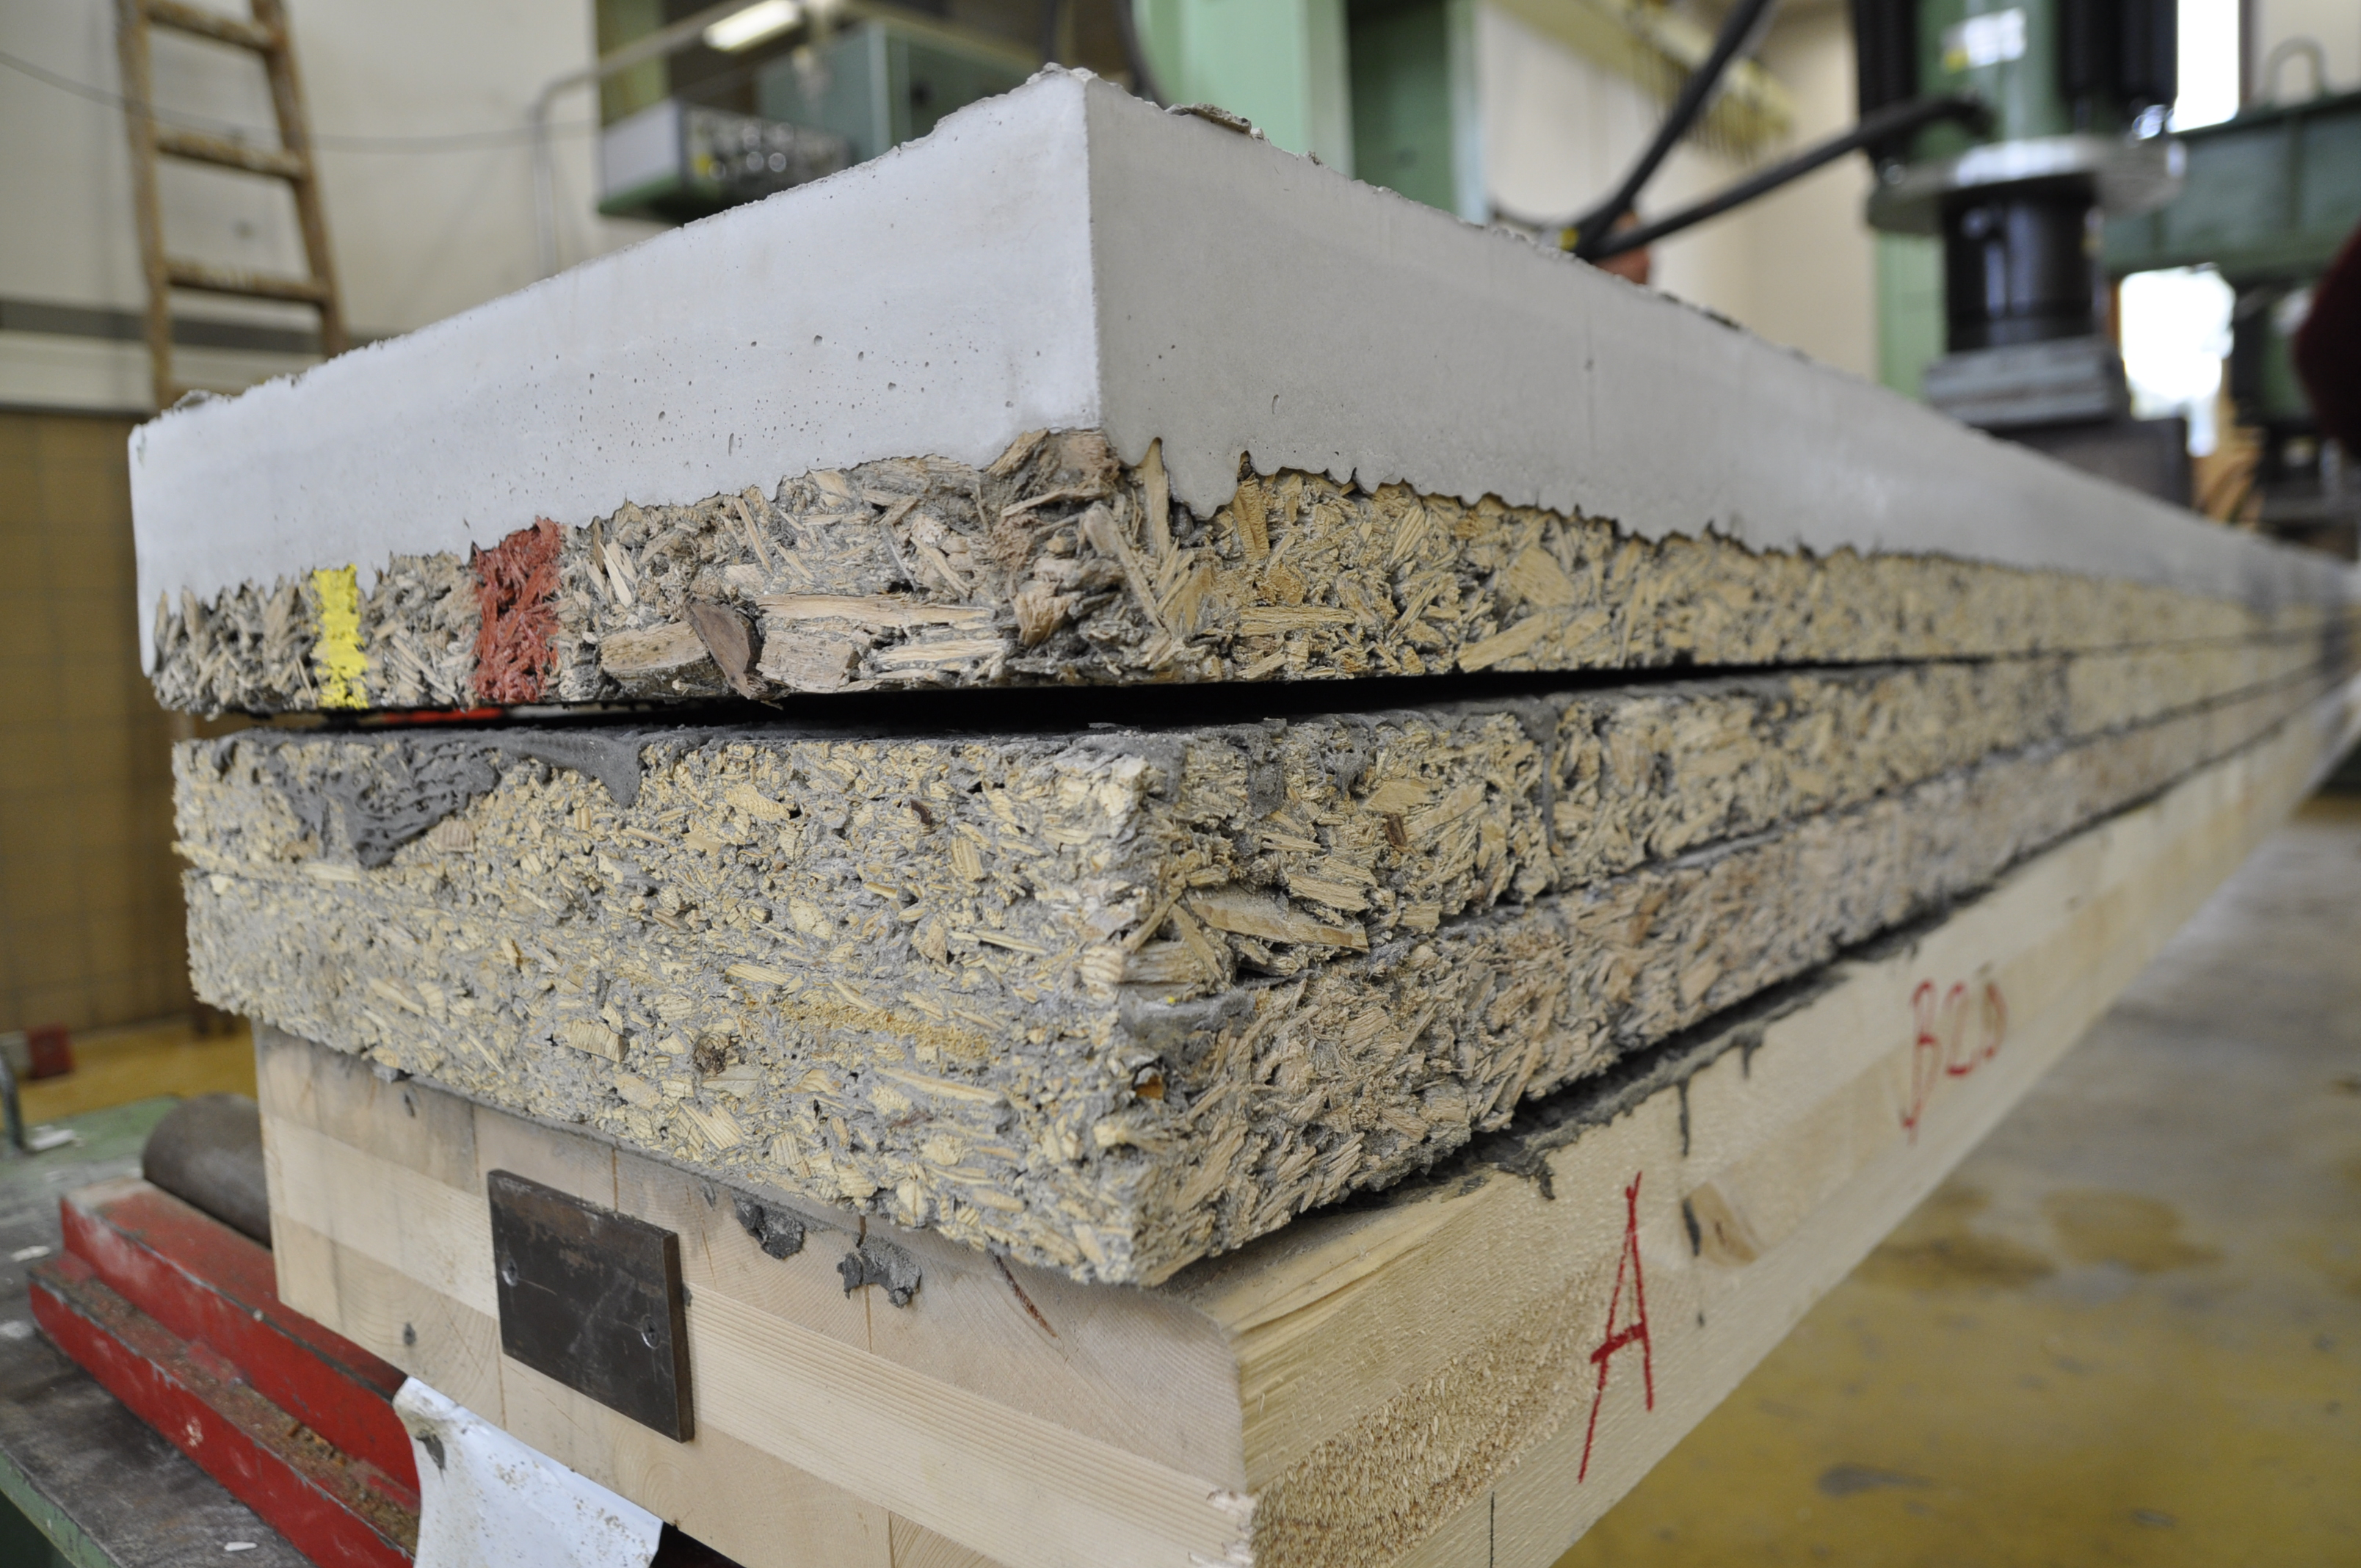
\includegraphics[scale =0.1]{Auswertung/2versuch/BT2_Verschiebung_AuflagerA.jpg}
\caption{Horizontale Verschiebung beim Auflager A, nach Maximalbelastung}
\label{BT2_Verschiebung_AuflagerA}
\end{center}
\end{figure}


\begin{figure}
\begin{center}
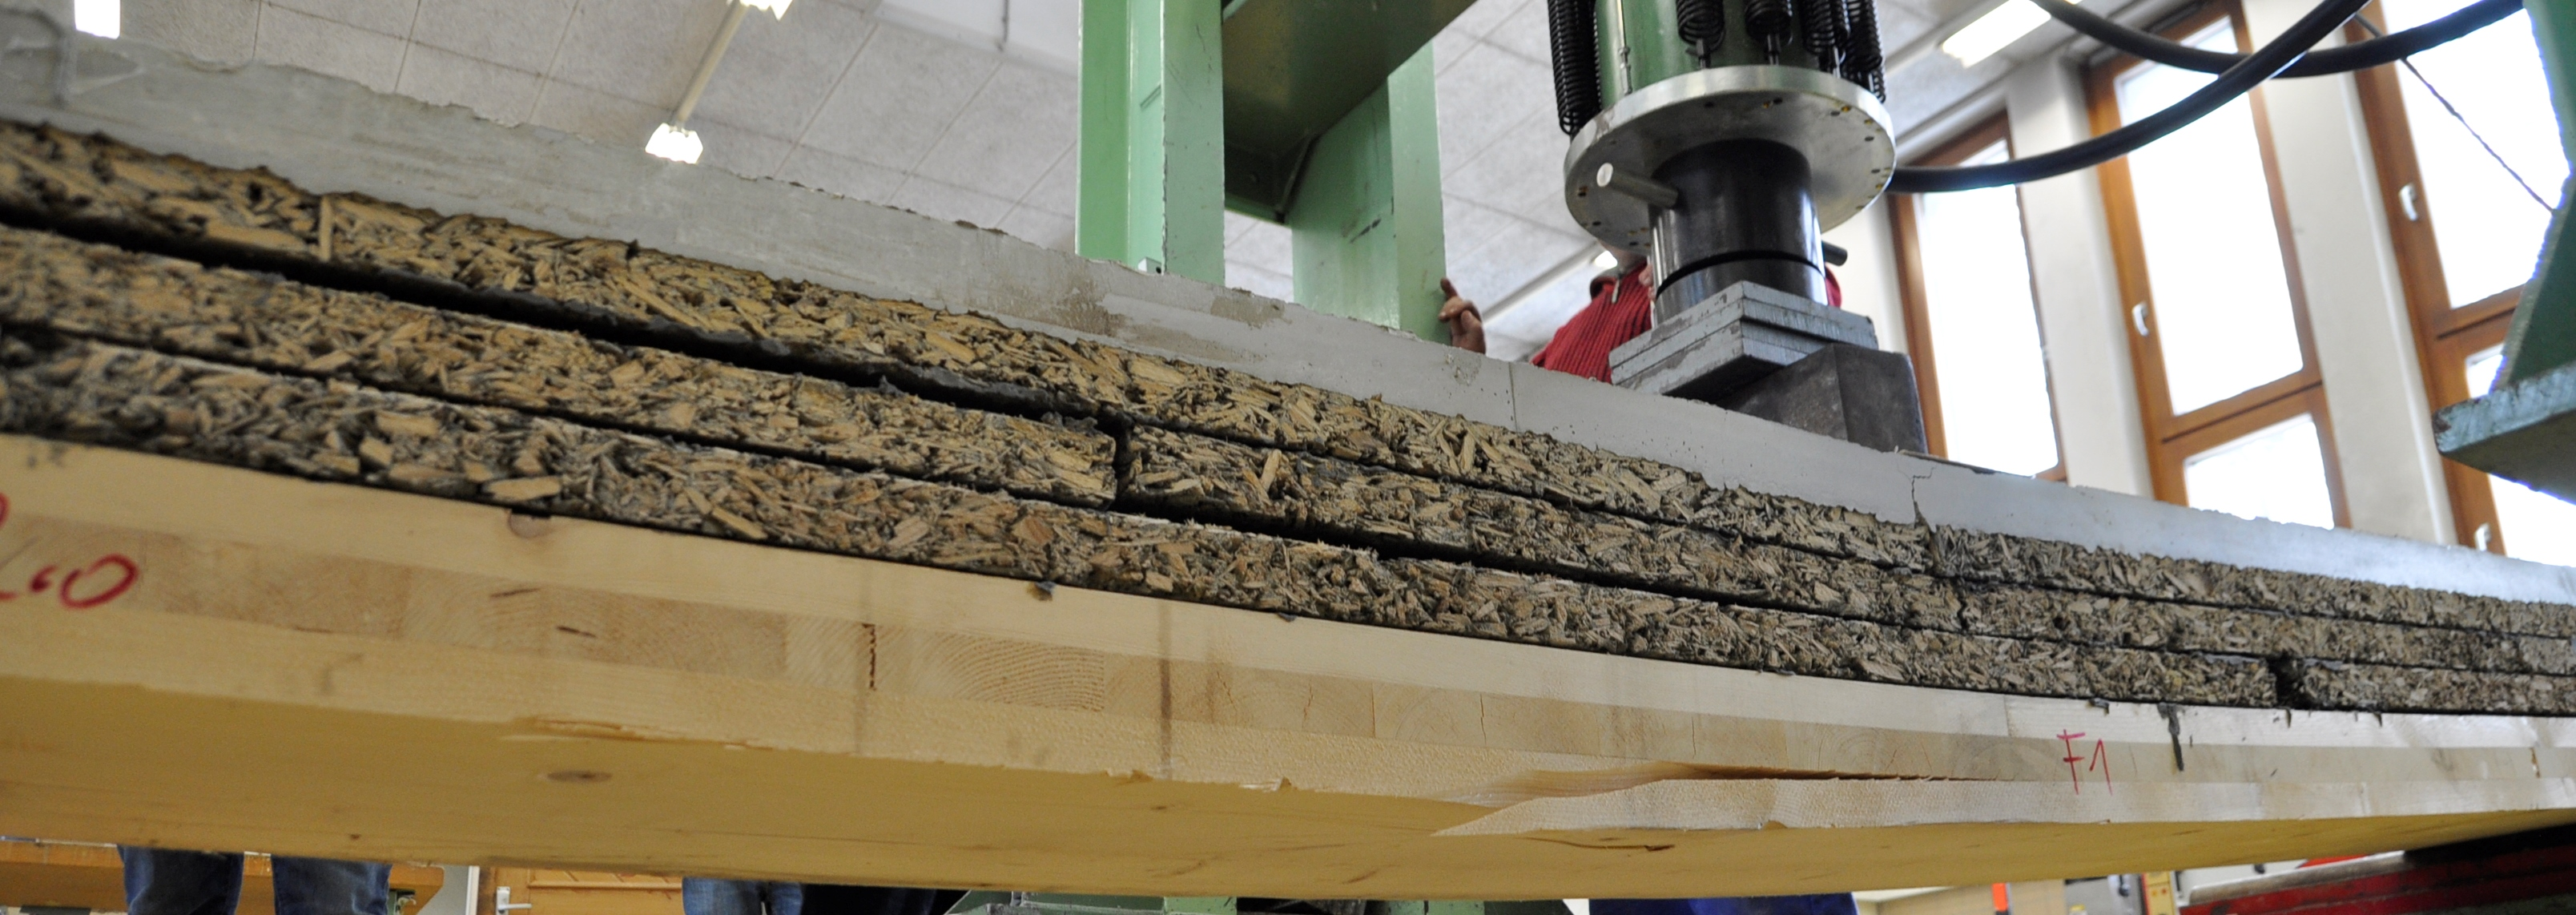
\includegraphics[scale =0.5]{Auswertung/2versuch/2versuch_versagen.jpg}
\caption{Darstellung des Versagen}
\label{2versuch versagen}
\end{center}
\end{figure}


\begin{figure}
\begin{center}
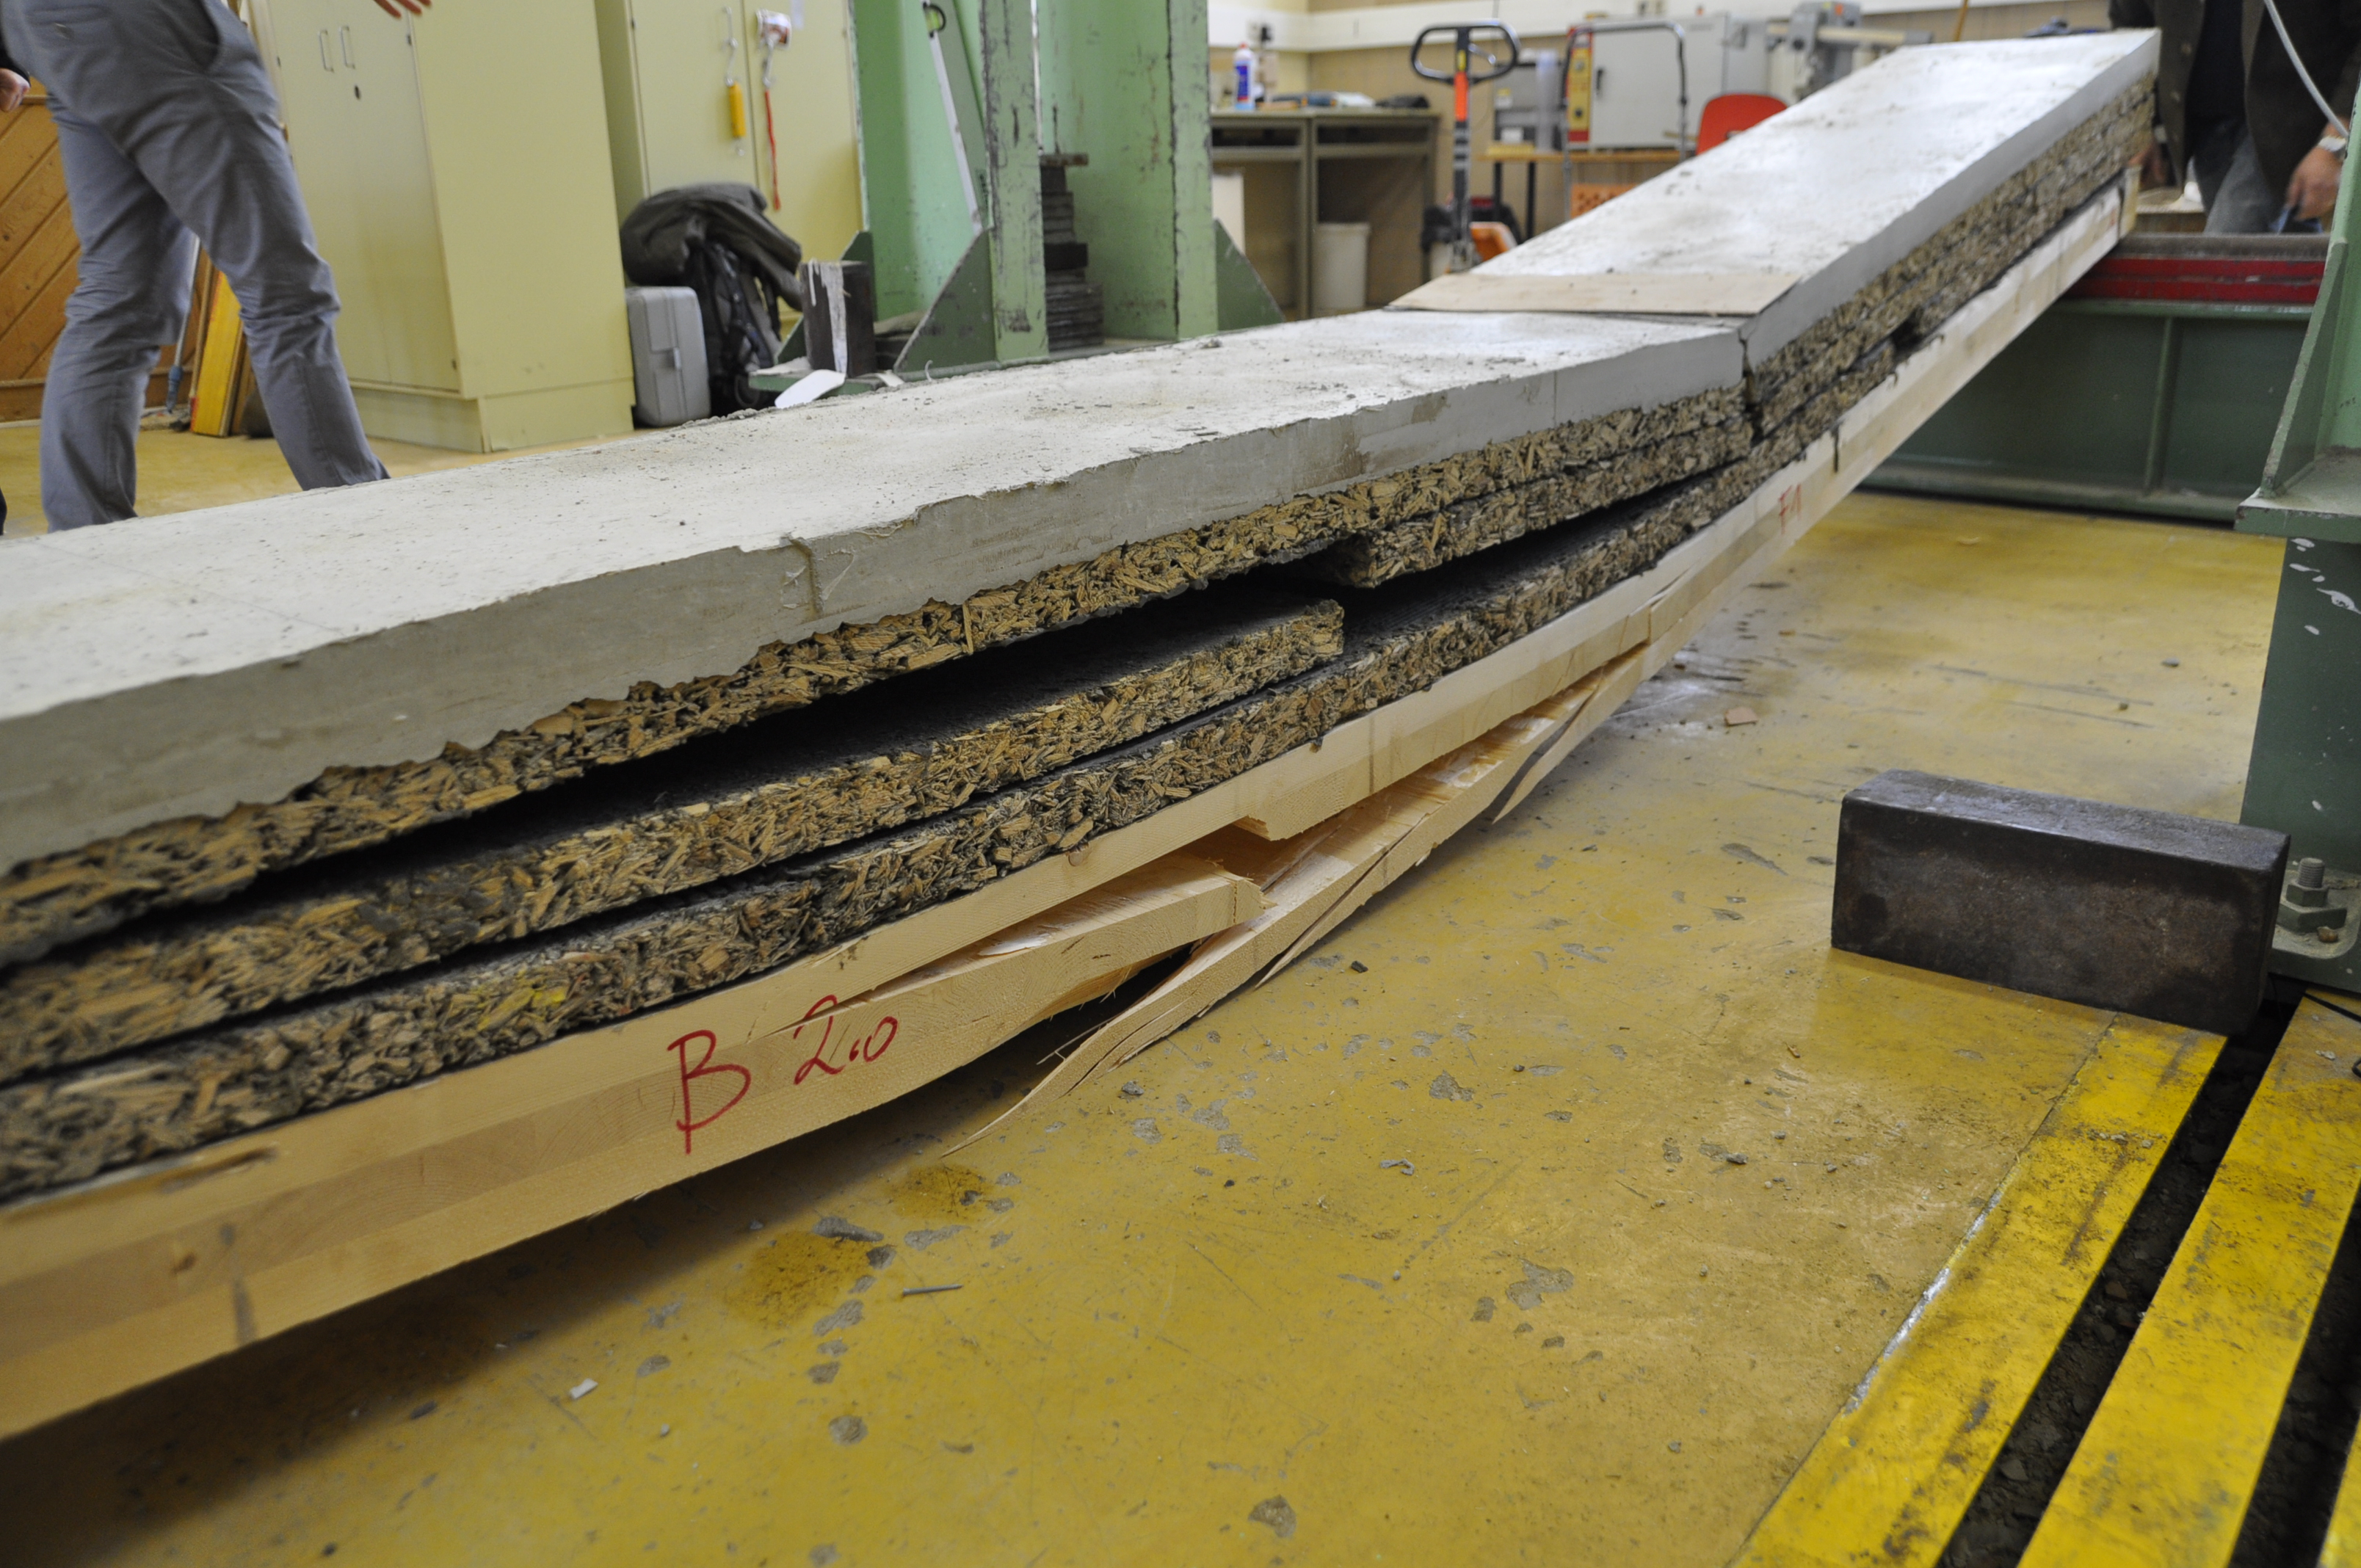
\includegraphics[scale =0.1]{Auswertung/2versuch/BT2_bruchbild.jpg}
\caption{Darstellung des vollständigen Bruchs}
\label{2versuch bruchbild}
\end{center}
\end{figure}


\begin{figure}[h]
\begin{minipage}[hbt]{7cm}	
	\includegraphics[width=7cm]{Auswertung/2versuch/2versuch_1oberfläche_velox.jpg}
	\caption{Oberfläche der aufgetragenen Schicht}
	\label{velos unten}
\end{minipage}
\hfill
\begin{minipage}[hbt]{7cm}
	\includegraphics[width=7cm]{Auswertung/2versuch/2versuch_2oberfläche_velox.jpg}
	\caption{Oberfläche der aufgelegten Schicht}
	\label{velox ober}
\end{minipage}
\end{figure}

\subsubsection{Verformungsverhalten}


In Abbildung \ref{2 Versuch: Kraft-Durchbiegung} ist die Arbeitslinie des Versuchs dargestellt.


Der Verlauf der Arbeitslinien ist bis zu einer Last von \unit[14]{kN} linear. Danach nehmen die Verformungen progressiv zu. Über der Belastung von \unit[16]{kN} vergrößert sich der Unterschied zwischen der Verschiebungslinien u2 und u3. Es ist auf die Abspaltung des Holzkeils der BSP-Platte zurückzuführen (Abbildung \ref{2versuch versagen}). 
 

Die relative Verschiebung zwischen der BSP-Schicht und der Betonschicht ist in Abbildung \ref{2_versuch_kraft_schubverschiebung} darstellt. Die Arbeitslinien sind nahezu ident. Sie weisen bis zu \unit[15]{kN} ein lineares Verhalten auf, danach ist ein progressiver Anstieg erkennbar.


\begin{figure}[h!]
\begin{center}
\begin{tikzpicture}
\begin{axis}[height=12cm, width=12cm, 
			no markers,
			xmajorgrids,ymajorgrids,
			xlabel=Verschiebung\,u\,$\lbrack mm \rbrack $,
			ylabel=Kraft\,/\,Zylinder\,$\lbrack kN\rbrack $,
			xmin=0,ymin=0,
			legend pos= south east
			]
\addplot table[y=F,x=u1]{Auswertung/2versuch/BT2.dat};
\addplot table[y=F,x=u2]{Auswertung/2versuch/BT2.dat};
\addplot table[y=F,x=u3]{Auswertung/2versuch/BT2.dat};
\legend{BT2\,u1,BT2\,u2,BT2\,u3}
\end{axis}
\end{tikzpicture}
\caption{Bauteilversuch 2: Kraft-Durchbiegung}
\label{2 Versuch: Kraft-Durchbiegung}
\end{center}
\end{figure}





\begin{figure}[h!]
\begin{center}
\begin{tikzpicture}
\begin{axis}[height=12cm, width=12cm,
			axis y line*=left, 
			no markers,
			xmajorgrids,ymajorgrids,
			xlabel=Zeit\,$\lbrack s \rbrack$,
			ylabel=Kraft\,/\,Zylinder\,$\lbrack kN\rbrack$,
			xmin=0,ymin=0,
			ymax=30,
			legend pos= north east			
			 ]
\addplot table[y=F,x=Time]{Auswertung/2versuch/BT2.dat};
\legend{F};
\end{axis}
\begin{axis}[height=12cm, width=12cm, 
			axis y line*=right,
			axis x line*=none,
			no markers,
			xmajorgrids,ymajorgrids,
			ylabel=Verschiebung\,u\,$\lbrack mm\rbrack$,
			xmin=0,ymin=0,
			ymax=60,
			legend pos=south east			
			 ]
\addplot table[y=u1,x=Time]{Auswertung/2versuch/BT2.dat};
\addplot table[y=u2,x=Time]{Auswertung/2versuch/BT2.dat};
\addplot table[y=u3,x=Time]{Auswertung/2versuch/BT2.dat};
\legend{BT2\,u1,BT2\,u2,BT2\,u3};
\end{axis}
\end{tikzpicture}
\caption{Bauteilversuch 2: Kraft-und Verschiebungsverlauf in Abhängigkeit von der Zeit}
\label{1 Versuch: Kraft-Durchbiegung-Zeit}
\end{center}
\end{figure}

\begin{figure}[h!]
\begin{center}
\begin{tikzpicture}
\begin{axis}[height=12cm, width=12cm, 
			no markers,
			xmajorgrids,ymajorgrids,
			xlabel=Verschiebung\,u\,$\lbrack mm \rbrack $,
			ylabel=Kraft\,/\,Zylinder\,$\lbrack kN\rbrack $,
			xmin=0,ymin=0,
			legend pos= south east
			]
\addplot table[y=F,x=u4]{Auswertung/2versuch/BT2.dat};
\addplot table[y=F,x=u5]{Auswertung/2versuch/BT2.dat};
\legend{BT2\,u4,BT2\,u5}
\end{axis}
\end{tikzpicture}
\caption{Bauteilversuch 2: Kraft-Schubverformung}
\label{2_versuch_kraft_schubverschiebung}
\end{center}
\end{figure}






\clearpage

\subsection{Bauteilversuch\,3\,(BT\,3)}

\subsubsection{Versuchskörper}
\label{abs:BT3_Versuchskoerper}

Der Schichtenaufbau ist in Abschnitt 2.1.2 beschrieben. 

Aufgrund der Erfahrungen, die mit dem Bauteil BT\,2 gemacht wurden, wurden folgende Änderungen bei den Verbindungsmitteln vorgenommen.

Die Anzahl und Anordnung der Schrauben ist der Abbildung \ref{3versuch} zu entnehmen. Im Auflagerbereich wurde eine zusätzliche Schraube angeordnet, um den Lastfall`"Einheben des Versuchskörpers in die Prüfanlage'" zu berücksichtigen.  

Weiters wurde ein Kleber mit höherer Steifigkeit (Sikatop 107) eingesetzt (siehe Kleberversuchsreihe\,2).


\begin{figure}[h!]
\begin{center}
\includegraphics[scale =0.9,trim= 1.5cm 10cm 1.5cm 10cm, clip=true]{Auswertung/3versuch/BT3.pdf}
\caption{Darstellung des BT\,3, mit Verbindungsmittel und Lasteinleiung}
\label{1versuch}
\end{center}
\end{figure}

\subsubsection{Versuchsablauf}


Wie im Abschnitt \ref{abs:Versuchsbaufaufbau_Durchführung} beschrieben, wurde der Versuch mit einer digitalen Messeinrichtung versehen und mithilfe einer programmierten Belastungskurve gesteuert. Abbildung \ref{3 Versuch: Kraft-Durchbiegung-Zeit} zeigt den zeitlichen Ablauf des Versuchs. 

Bei der Last von \unit[35]{kN} wurde ein weiterer Haltepunkt mit einer Dauer von \unit[30]{min} eingefügt, um das kurzzeitige Kriechverhalten  unter hoher Last zu beobachten.

Anschließend wurde der Bauteil weiter belastet, bis ein deutlicher Lastabfall eintrat. Die Maximallast betrug \unit[58]{kN}.

Nach Entfernung der Messinstrumente wurde der Bauteil manuell gesteuert belastet, bis die BSP-Platte bei einer Last von \unit[35]{kN} im Bereich der Lasteinleitung $F_B$ brach.

 



 

\begin{figure}[h!]
\begin{minipage}[hbt]{7cm}	
	\includegraphics[width=7cm]{Auswertung/3versuch/beton_veloxriss.jpg}
	\caption{Darstellung des Risse im Beton und Holzbeton}
	\label{beton_veloxriss}
\end{minipage}
\hfill
\begin{minipage}[hbt]{7cm}
	\includegraphics[width=7cm]{Auswertung/3versuch/fuge.jpg}
	\caption{Spalt zwischen BSP und Holzbeton}
	\label{spalt}
\end{minipage}
\end{figure}


\begin{figure}
\begin{center}
	\includegraphics[scale=0.1]{Auswertung/3versuch/bruch_3versuch.jpg}
	\caption{Bruch nach Wiederbelastung bei Lasteinleitung $F_B$  }
	\label{bruch_3versuch}
\end{center}
\end{figure}




\begin{figure}
\begin{center}
	\includegraphics[width=6cm]{Auswertung/3versuch/fugenbruch_3versuch.jpg}
	\caption{Oberflächbild: BSP-Platte und Holzspanbeton}
	\label{fugenbruch_3versuch}
\end{center}
\end{figure}

\subsubsection{Versagensbeschreibung}

Die erste Schädigung trat als Riss im Beton und im Holzbeton im Bereich der Lasteinleitung $F_{B}$ bei der Maximallast von \unit[58]{kN} auf (Abbildung \ref{beton_veloxriss}). Dieser Betonzugriss ist ein Resultat der Spannungsumlagerung, welche sich zufolge des Versagens der Holzschrauben einstellt. Dieser Verlust der Verbundwirkung ist auch im Diagramm in Abbildung \ref{3 Versuch: Kraft-Schubverformung} zu sehen. Die Relativverschiebung zwischen Holz und Beton bei Auflager B (u4) erhöht sich im Bereich der Maximallast progressiv.

Abbildung \ref{fugenbruch_3versuch} zeigt eine gute Verklebung im Mittelbereich des Bauteils, hier versagte das Velox. In den Randbereichen versagte hingegen die Klebefuge. 


\begin{figure}
\begin{center}
\begin{tikzpicture}
\begin{axis}[	legend pos= south east,
				height=12cm, width=12cm,
				no markers,
				xmajorgrids,ymajorgrids,
				xlabel=Verschiebung\, u \,$\lbrack mm \rbrack $  ,
				ymin=0,xmin=0,
				ylabel=Kraft\, / \,Zylinder\, $\lbrack kN\rbrack $
				]
\addplot table[y=F,x=u1]{Auswertung/3versuch/BT3.dat};
\addplot table[y=F,x=u2]{Auswertung/3versuch/BT3.dat};
\addplot table[y=F,x=u3]{Auswertung/3versuch/BT3.dat};
\legend{BT3\,u1,BT3\,u2,BT3\,u3}
\end{axis}
\end{tikzpicture}
\caption{Bauteilversuch 3: Kraft-Durchbiegung}
\label{3 Versuch: Kraft-Durchbiegung}
\end{center}
\end{figure}


\begin{figure}[h!]
\begin{center}
\begin{tikzpicture}
\begin{axis}[height=12cm, width=12cm,
			axis y line*=left, 
			no markers,
			xmajorgrids,ymajorgrids,
			xlabel=Zeit\,$\lbrack s \rbrack$,
			ylabel=Kraft\,/\,Zylinder\,$\lbrack kN\rbrack$,
			xmin=0,ymin=0,
			ymax=60,
			legend pos= north east			
			 ]
\addplot table[y=F,x=Time]{Auswertung/3versuch/BT3.dat};
\legend{F};
\end{axis}
\begin{axis}[height=12cm, width=12cm, 
			axis y line*=right,
			axis x line*=none,
			no markers,
			xmajorgrids,ymajorgrids,
			ylabel=Verschiebung\,u\,$\lbrack mm\rbrack$,
			xmin=0,ymin=0,
			ymax=60,
			legend pos=south east			
			 ]
\addplot table[y=u1,x=Time]{Auswertung/3versuch/BT3.dat};
\addplot table[y=u2,x=Time]{Auswertung/3versuch/BT3.dat};
\addplot table[y=u3,x=Time]{Auswertung/3versuch/BT3.dat};
\legend{BT3\,u1,BT3\,u2,BT3\,u3};
\end{axis}
\end{tikzpicture}
\caption{Bauteilversuch 3: Kraft-und Verschiebungsverlauf in Abhängigkeit von der Zeit}
\label{3 Versuch: Kraft-Durchbiegung-Zeit}
\end{center}
\end{figure}





\begin{figure}
\begin{center}
\begin{tikzpicture}
\begin{axis}[	legend pos= south east,
				height=12cm, width=12cm,
				no markers,
				xmajorgrids,ymajorgrids,
				xlabel=Verschiebung\, u \,$\lbrack mm \rbrack $  ,
				ymin=0,xmin=0,
				ylabel=Kraft\, / \,Zylinder\, $\lbrack kN\rbrack $
				]
\addplot table[y=F,x=u4]{Auswertung/3versuch/BT3.dat};
\addplot table[y=F,x=u5]{Auswertung/3versuch/BT3.dat};
\legend{BT3\,u4,BT3\,u5}
\end{axis}
\end{tikzpicture}
\caption{Bauteilversuch 3: Kraft-Schubverformung}
\label{3 Versuch: Kraft-Schubverformung}
\end{center}
\end{figure}

\subsubsection{Verformungsverhalten}

In Abbildung \ref{3 Versuch: Kraft-Durchbiegung} ist die Arbeitslinie des Versuchs dargestellt.


Der Verlauf der Arbeitslinien ist bis zu einer Last von \unit[50]{kN} linear. Anschließend nehmen die Verformungen progressiv zu. Die Verschiebungen u2 und u3 haben bis zur Last von \unit[56]{kN} den gleichen Verlauf, danach nimmt die Verformung u3 stärker zu. Dieses Verhalten ist auf das Versagen der Schubverbindungen in diesem Bereich zurückzuführen. 

In der Abbildung \ref{3 Versuch: Kraft-Schubverformung} ist die Schubverformung des Versuchs abgebildet. Durch die geringe Auflösung der Messsensoren entstand die Treppenkurve. Dennoch ist ein annähernd linearer Verlauf bis zur Last von ca.\ \unit[50]{kN} zu erkennen. Wie im vorigen Abschnitt beschrieben zeigt die Zunahme der Verschiebung u4 ein Versagen der Schubverbindungen im Bereich des Auflager B an.



\clearpage
\subsection{Bauteilversuch\,4\,(BT\,4)}

\subsubsection{Versuchskörper}

Der Schichtenaufbau ist in Abschnitt 2.1.2 beschrieben. 

Diese Probe wurde ohne mechanische Verbindungsmittel (Schrauben) gefertigt, um einen Referenzwert und den Einfluss der Schrauben auf das System zu ermitteln.

Bei diesem Versuch wurde wie bei Bauteil BT\,3 der Kleber SikaTop 107 verwendet.

\begin{figure}[h!]
\begin{center}
\includegraphics[scale =0.9,trim= 1.5cm 10cm 1.5cm 10cm, clip=true]{Auswertung/4versuch/BT4.pdf}
\caption{Darstellung des BT\,4, mit Verbindungsmittel und Lasteinleiung}
\label{1versuch}
\end{center}
\end{figure}



\begin{figure}[h]
\begin{center}
\includegraphics[scale =0.8]{Auswertung/4versuch/schaden_im_endbereich.jpg}
\caption{Stahlblech durchdringt die unterste Klebefuge, bis zu \unit[20]{cm} vom Bauteilende}
\label{4versuch_Stahlblech_Klebefuge}
\end{center}
\end{figure}
\subparagraph{Schädigungen vor Versuchsdurchführung}
\label{abs:BT4_Schaden}


\begin{figure}
\begin{center}
\includegraphics[scale =0.05]{Auswertung/4versuch/riss.jpg}
\caption{Rissdarstellung in der unteren Klebefuge}
\label{riss}
\end{center}
\end{figure}

\subsubsection{Versuchsablauf}


Wie im Abschnitt \ref{abs:Versuchsbaufaufbau_Durchführung} beschrieben, wurde der Versuch mit einer digitalen Messeinrichtung versehen und mithilfe einer programmierten Belastungskurve gesteuert. Abbildung \ref{4 Versuch: Kraft-Durchbiegung-Zeit} zeigt den zeitlichen Ablauf des Versuchs. 

Bei der Last von \unit[5,4]{kN} war ein Haltepunkt von \unit[120]{s} vorgesehen. Jedoch begann der Bauteil bei dieser Laststufe zu kriechen, daher wurde die Last ca.\ \unit[900]{s} manuell gehalten. In Abbildung \ref{4 Versuch: Kraft-Durchbiegung-Zeit} ist dargestellt, dass bei konstanter Last die Verformungen zunehmen (bei $t=400 - \unit[600]{s}$).

Anschließend wurde der Versuch nach der programmierten Belastungskurve weiter gefahren, bis er bei der Last von \unit[7,5]{kN} beendet wurde, um die Messinstrumente abzunehmen.

Nach Entfernung der Messinstrumente wurde der Bauteil nochmals belastet, bis die BSP-Platte bei einer Last von \unit[12]{kN} in Trägermitte brach.

\begin{figure}[h]
\begin{minipage}[hbt]{7cm}	
	\includegraphics[width=7cm]{Auswertung/4versuch/4versuch_versagen.jpg}
	\caption{Darstellung des horizontalen Verschiebung beim Auflager A}
	\label{4versuch_versagen}
\end{minipage}
\hfill
\begin{minipage}[hbt]{7cm}
	\includegraphics[width=7cm]{Auswertung/4versuch/4versuch_schichtbruch.jpg}
	\caption{Risse in der Beton-und Veloxschicht}
	\label{4versuch_schichtbruch}
\end{minipage}
\end{figure}



\subsubsection{Versagensbeschreibung}

Durch den fehlerhaften Verbund in der Klebefuge kam es zu Zugrissen im Beton und im Holzbeton in der Nähe der Lasteinleitung $F_B$ bei einer Last von \unit[5]{kN}(Abbildung \ref{4versuch_schichtbruch}). 

Beim Zeitpunkt \unit[600]{s} bildete sich ein weiterer Riss in Trägermitte und die unterste Verbundfuge löste sich vollständig von Trägermitte bis zum Auflager B.
Dadurch nahmen die Verformungen sprunghaft zu, insbesondere die Relativverschiebung u5.

Das Versagen der BSP-Platte fand bei Wiederbelastung bei \unit[12]{kN} statt.


\begin{figure}
\begin{center}
\begin{tikzpicture}
\begin{axis}[	legend pos= south east,
				height=12cm, width=12cm,
				no markers,
				xmajorgrids,ymajorgrids,
				xlabel=Verschiebung\, u \,$\lbrack mm \rbrack $  ,
				ymin=0,xmin=0,
				ylabel=Kraft\, / \,Zylinder\, $\lbrack kN\rbrack $
				]
\addplot table[y=F,x=u1]{Auswertung/4versuch/BT4.dat};
\addplot table[y=F,x=u2]{Auswertung/4versuch/BT4.dat};
\addplot table[y=F,x=u3]{Auswertung/4versuch/BT4.dat};
\legend{BT4\,u1,BT4\,u2,BT4\,u3}
\end{axis}
\end{tikzpicture}
\caption{Bauteilversuch 4: Kraft-Durchbiegung}
\label{4 Versuch: Kraft-Durchbiegung}
\end{center}
\end{figure}
BT4-5.4kN.dat

\begin{figure}
\begin{center}
\begin{tikzpicture}
\begin{axis}[	legend pos= south east,
				height=12cm, width=12cm,
				no markers,
				xmajorgrids,ymajorgrids,
				xlabel=Verschiebung\, u \,$\lbrack mm \rbrack $  ,
				ymin=0,xmin=0,
				ylabel=Kraft\, / \,Zylinder\, $\lbrack kN\rbrack $
				]
\addplot table[y=F,x=u1]{Auswertung/4versuch/BT4-5.4kN.dat};
\addplot table[y=F,x=u2]{Auswertung/4versuch/BT4-5.4kN.dat};
\addplot table[y=F,x=u3]{Auswertung/4versuch/BT4-5.4kN.dat};
\legend{BT4\,u1,BT4\,u2,BT4\,u3}
\end{axis}
\end{tikzpicture}
\caption{Bauteilversuch 4: Kraft-Durchbiegung bis \unit[5,4]{kN}}
\label{4 Versuch: Kraft-Durchbiegung-5,4kN}
\end{center}
\end{figure}





\begin{figure}[h!]
\begin{center}
\begin{tikzpicture}
\begin{axis}[height=12cm, width=12cm,
			axis y line*=left, 
			no markers,
			xmajorgrids,ymajorgrids,
			xlabel=Zeit\,$\lbrack s \rbrack$,
			ylabel=Kraft\,/\,Zylinder\,$\lbrack kN\rbrack$,
			xmin=0,ymin=0,
			ymax=9,
			legend pos= north east			
			 ]
\addplot table[y=F,x=Time]{Auswertung/4versuch/BT4.dat};
\legend{F};
\end{axis}
\begin{axis}[height=12cm, width=12cm, 
			axis y line*=right,
			axis x line*=none,
			no markers,
			xmajorgrids,ymajorgrids,
			ylabel=Verschiebung\,u\,$\lbrack mm\rbrack$,
			xmin=0,ymin=0,
			ymax=90,
			legend pos=south east			
			 ]
\addplot table[y=u1,x=Time]{Auswertung/4versuch/BT4.dat};
\addplot table[y=u2,x=Time]{Auswertung/4versuch/BT4.dat};
\addplot table[y=u3,x=Time]{Auswertung/4versuch/BT4.dat};
\legend{BT4\,u1,BT4\,u2,BT4\,u3};
\end{axis}
\end{tikzpicture}
\caption{Bauteilversuch 4: Kraft-und Verschiebungsverlauf in Abhängigkeit von der Zeit}
\label{4 Versuch: Kraft-Durchbiegung-Zeit}
\end{center}
\end{figure}


\subsubsection{Verformungsverhalten}

In Abbildung \ref{4 Versuch: Kraft-Durchbiegung} ist die Arbeitslinie des Versuchs dargestellt.


Der Verlauf der Arbeitslinien weist schon bei geringer Belastung auf ein nichtlineares Verhalten hin. Beim Haltepunkt \unit[2,7]{kN} ist ein Kriechverhalten ersichtlich.

Der weitere Verlauf bis zum nächsten Haltepunkt \unit[5,4]{kN} zeigt ebenfalls ein deutlich nichtlineares Verhalten

Bei der konstant gehaltenen Last von \unit[5,4]{kN} nimmt die Verschiebungen ständig zu, dass auf ein ausgeprägtes Kriechverhalten hinweist.


Nach der Entlastung auf \unit[2,7]{kN} und darauffolgenden Wiederbelastung ist erkennbar, dass der Bauteil sich plastisch verformt hat. 





In der Abbildung \ref{4 Versuch: Kraft-Schubverformung} ist die Schubverformung des Versuchs abgebildet. 

 
 Die Kennlinien sind bis zu dem Lastniveau von \unit[5,4]{kN} fast ident. Bei der konstanten Last von \unit[5,4]{kN} steigt die Verschiebung der Kennlinie u5 erheblich an. Dies ist auf das Versagen der Verbundfuge im Bereich zwischen Trägermitte und dem Auflager B zurück zu führen.

  



\begin{figure}
\begin{center}
\begin{tikzpicture}
\begin{axis}[	legend pos= south east,
				height=12cm, width=12cm,
				no markers,
				xmajorgrids,ymajorgrids,
				xlabel=Verschiebung\, u \,$\lbrack mm \rbrack $  ,
				ymin=0,xmin=0,
				ylabel=Kraft\, / \,Zylinder\, $\lbrack kN\rbrack $
				]
\addplot table[y=F,x=u4]{Auswertung/4versuch/BT4.dat};
\addplot table[y=F,x=u5]{Auswertung/4versuch/BT4.dat};
\legend{BT4\,u4,BT4\,u5}
\end{axis}
\end{tikzpicture}
\caption{Bauteilversuch 4: Kraft-Schubverformung}
\label{4_versuch_kraft_schubverschiebung}
\end{center}
\end{figure}




\clearpage
\subsection{Gegenüberstellung der Bauteilversuche}




\begin{figure}[h!]
\begin{center}
\begin{tikzpicture}
\begin{axis}[height=12cm, width=12cm, 
			no markers,
			xmajorgrids,ymajorgrids,
			xlabel=Verschiebung $\lbrack mm \rbrack $ ,
			xmin=0,ymin=0,
			ylabel=Kraft\,$\lbrack kN \rbrack $,
			legend pos= north west
			]
\addplot table[y=F,x=u1.1]{Auswertung/1versuch/BT1.dat};
\addplot table[y=F,x=u1]{Auswertung/2versuch/BT2.dat};
\addplot table[y=F,x=u1]{Auswertung/3versuch/BT3.dat};
\addplot table[y=F,x=u1]{Auswertung/4versuch/BT4.dat};
\legend{BT1\,u1,BT2\,u1,BT3\,u1,BT4\,u1}
\end{axis}
\end{tikzpicture}
\caption{Vergleich der vertikalen Verschiebung in der Bauteilmitte}
\label{Vergleich_durchbiegung}
\end{center}
\end{figure}


\begin{figure}[h!]
\begin{center}
\begin{tikzpicture}
\begin{axis}[height=12cm, width=12cm, 
			no markers,
			xmajorgrids,ymajorgrids,
			xlabel=Verschiebung $\lbrack mm \rbrack $ ,
			xmin=0,ymin=0,
			ylabel=Kraft\,$\lbrack kN \rbrack $,
			legend pos= north west
			]
\addplot table[y=F1,x=BT1u1]{Auswertung/vergleiche/vergleich_durchbiegung.dat};
\addplot table[y=F2,x=BT2u1]{Auswertung/vergleiche/vergleich_durchbiegung.dat};
\addplot table[y=F3,x=BT3u1]{Auswertung/vergleiche/vergleich_durchbiegung.dat};
\addplot table[y=F4,x=BT4u1]{Auswertung/vergleiche/vergleich_durchbiegung.dat};
\legend{BT1\,u1,BT2\,u1,BT3\,u1,BT4\,u1,ul}
\end{axis}
\end{tikzpicture}
\caption{Vergleich der vertikalen Verschiebung in der Bauteilmitte bis 10 kN}
\label{Vergleich_durchbiegung10}
\end{center}
\end{figure}


\begin{figure}[h!]
\begin{center}
\begin{tikzpicture}
\begin{axis}[height=12cm, width=12cm, 
			no markers,
			xmajorgrids,ymajorgrids,
			xlabel=Verschiebung $\lbrack mm \rbrack $ ,
			xmin=0,ymin=0,
			ylabel=Kraft\,$\lbrack kN \rbrack $,
			legend pos= north east
			]
\addplot [blue,solid] table[y=F1,x=BT1u4]{Auswertung/vergleiche/vergleich_schubverformung1.dat};
\addplot [blue,densely dashed] table[y=F1,x=BT1u5]{Auswertung/vergleiche/vergleich_schubverformung1.dat};
\addplot [red,solid] table[y=F2,x=BT2u4]{Auswertung/vergleiche/vergleich_schubverformung1.dat};
\addplot [red,densely  dashed] table[y=F2,x=BT2u5]{Auswertung/vergleiche/vergleich_schubverformung1.dat};
\addplot [brown!60!black,solid] table[y=F3,x=BT3u4]{Auswertung/vergleiche/vergleich_schubverformung1.dat};
\addplot [brown!60!black,densely  dashed] table[y=F3,x=BT3u5]{Auswertung/vergleiche/vergleich_schubverformung1.dat};
\addplot [black,solid] table[y=F4,x=BT4u4]{Auswertung/vergleiche/vergleich_schubverformung1.dat};
\addplot [black,densely  dashed] table[y=F4,x=BT4u5]{Auswertung/vergleiche/vergleich_schubverformung1.dat};
\legend{BT1\,u4,BT1\,u5,BT2\,u4,BT2\,u5,BT3\,u4,BT3\,u5,BT4\,u4,BT4\,u5}
\end{axis}
\end{tikzpicture}
\caption{Vergleich der horizontalen Verschiebung beim Auflager }
\label{vergleich-schubverformung}
\end{center}
\end{figure}



\begin{table}[h]
\caption{Vergleich der Bauteilversuche (Maximallast, Durchbiegung, Biegesteifigkeit)}
\begin{center}
\begin{tabular}{|c|c|c|c|c|}
\hline 
Versuch & $F_{max}$  & $F(w=l/400)$ & $w(F=\unit[8]{kN})$ & $EI_{equ}$ \\ 

& [kN] & [kN] & [mm]   & [$\unit{kN \cdot cm^2}$] \\ 
\hline\hline
1 & 72 & 25 & 5,5 & 1555200  \\ 
\hline 
2  & 30 & 15 & 9,20 & 929739 \\ 
\hline 
3 & 58 & 24,4 & 6,2 & 1379613 \\ 
\hline 
4  & 12 & 4,8 & 58 & 147476 \\ 
\hline 
\end{tabular} 
\end{center}
\label{tab:vergleich_versuche}
\end{table}


\begin{figure}
\begin{center}

\begin{tikzpicture}
\pgfplotsset{small}
\matrix{
\begin{axis}[
			title = $F_{max}$,
			ylabel= $\lbrack kN\rbrack $,
			ybar,
			enlargelimits=0.25,
			symbolic x coords={BT1,BT2,BT3,BT4},
			xtick=data,
			nodes near coords
			]
\addplot coordinates {(BT1,72) (BT2,30) (BT3,58) (BT4,12)};
\end{axis}

&

\begin{axis}[
			title = $F_{w=l/400}$,
			ylabel= $\lbrack kN\rbrack $ ,
			ybar,
			enlargelimits=0.25,
			symbolic x coords={BT1,BT2,BT3,BT4},
			xtick=data,
			nodes near coords
			]
\pgfplotsset{cycle list shift=1}
\addplot coordinates {(BT1,25) (BT2,15) (BT3,24) (BT4,5.0)};
\end{axis}

\\

\begin{axis}[
			title = $w_{max \left( F=8kN \right) }$,
			ylabel= $\lbrack mm\rbrack $ ,
			ybar,
			enlargelimits=0.25,
			symbolic x coords={BT1,BT2,BT3,BT4},
			xtick=data,
			nodes near coords
			]
\pgfplotsset{cycle list shift=2}
\addplot coordinates {(BT1,5.5) (BT2,9.2) (BT3,6.2) (BT4,58)};
\end{axis}

&

\begin{axis}[
			title = $EI_{equ}$,
			ylabel= $\lbrack MN \cdot m^2\rbrack $ ,
			ybar,
			enlargelimits=0.25,
			symbolic x coords={BT1,BT2,BT3,BT4},
			xtick=data,
			nodes near coords
			]
\pgfplotsset{cycle list shift=3}
\addplot coordinates {(BT1,0.155) (BT2,0.092) (BT3,0.138) (BT4,0.015)};
\end{axis}

\\
};
\end{tikzpicture} 
\caption{Vergleich der Bauteilversuche (Maximallast, Durchbiegung, Biegesteifigkeit)}
\label{abb:vergleich_balkendiagramm}

\end{center}
\end{figure}

\subsubsection{Durchbiegung in Feldmitte}
In der Abbildung \ref{vergleich-durchbiegung} sind die Durchbiegungskennlinien in Trägermitte darstellt.
Es fällt auf, das die Arbeitslinien der BT1 und BT3 eine sehr gute Übereinstimmung aufweisen. Der Bauteil 2 hat eine geringere Biegesteifigkeit als diese beiden Versuchskörper. Der Träger BT\,4 hatte die geringste Biegesteifigkeit.

Um das Verformungs- und das Traglastverhalten der Sandwichbauteile zu analysieren, werden die Messwerte für eine Durchbiegung von $w=\nicefrac{l}{400}$ und eine Belastung von $F=\unit[8]{kN}$ als Vergleichswerte herangezogen. Der Wert für die Durchbiegung wurde so gewählt, dass Reserven für Langzeitverformungen gegeben sind. Der Belastungswert ergibt sich aus der Summe der Eigenlast und einer üblichen Nutzlast im Wohn- und Bürobau (Tabelle \ref{tab:vergleich_versuche} und Abbildung \ref{abb:vergleich_balkendiagramm}).

Die Maximallast verhält sich analog zu den Biegesteifigkeiten. Die Bauteile mit höherer Biegesteifigkeit $EI_{equ}$ haben auch eine höhere Maximallast $F_{max}$. 

Die Werte $w_{max, F=\unit[8]{kN}}$ und $EI_{equ}$ für den Bauteil BT\,4 weichen stark von den restlichen Werten ab, weil der Bauteil in diesem Zustand bereits versagt.

\subsubsection{Schubverformung}
Abbildung \ref{vergleich-schubverformung} vergleicht die Relativverschiebungen zwischen Beton und Holz in Abhängigkeit der Kraft an beiden Auflagern aller Bauteilversuche. Da die Verbundsteifigkeit der Schichten zwischen Beton und Holz entscheidenden Einfluss auf das Verformungs- und Tragverhalten des Sandwichbauteils hat, ist die Biegesteifigkeit der Systeme mit geringer Schubverformung am höchsten.
Dieser Zusammenhang wird auch durch die Anwendung des $\gamma$-Verfahrens als Berechnungsmodell anschaulich dargestellt (Abschnitt ????). 

\clearpage
\section{Schubversuch}
\label{abs:schubversuch}

Wie im vorigen Abschnitt erläutert, hat das Schubverhalten der Zwischenschichten zwischen Beton und Holzschicht großen Einfluss sowohl auf die Verteilung der Schnittgrößen, als auch auf das Verformungsverhalten des Sandwichbauteils.

Mit den Versuchen, die dieser Abschnitt beschreibt, kann das Schubverhalten des Systems erforscht werden.

Bei Versuchskörper BT\,1 fand das Versagen zwischen Auflager A und Lasteinleitung $F_A$ statt. In der Nähe der Lasteinleitung brach die BSP-Platte vollständig durch. Der Rest des Trägers von Lasteinleitungspunkt $F_A$ bis Auflager B hatte keine sichtbare Schädigung.

In Anlehnung an die Schubversuche in ????Literatur wurden die Versuche geplant. Für die Probekörper wurden Abschnitte des Trägers BT\,1 gewählt, in denen sich jeweils drei Schraubenpaare befanden. Mit Hilfe einer Motorsäge und einer Flex (Trennschleifer) wurde der restliche Träger zerteilt.
In Abbildung \ref{träger_scherversuch} ist ersichtlich, welche Teile des Trägers verwendet wurden. 



\begin{figure}[h]
\begin{center}
\includegraphics[scale =0.8,trim= 1cm 12cm 1cm 12cm, clip=true]{Auswertung/schubversuch/Teile_Schubversuch.pdf}
\caption{Darstellung des verwendeten Teiles der Trägers}
\label{träger_scherversuch}
\end{center}
\end{figure}



Aus ???LitVerweis
\begin{quote}
Hinsichtlich der Ermittlung von Scher- bzw. Schubfestigkeiten für den Baustoff Holz
existiert die Problematik, dass es nahezu unmöglich ist, einen reinen Schubspannungszustand
für Scherflächen parallel zur Faser zu erzeugen. Bereits Petermann
[Pet41] und Kollmann [Kol82] erkannten dieses Problem und betrachteten verschiedene
Ansätze zur Lösung desselben. Bis heute - weitere 70 Jahre nach Erscheinen der
oben genannten Arbeiten - ist diese Problematik nicht abschließend gelöst.

Im Wesentlichen haben sich heute zwei Prüfverfahren zur Ermittlung der Schubfestigkeit
von Holz etabliert, welche den einschlägigen Normen in verschiedenen Ländern
zugrunde liegen. Im Europäischen Raum bezieht sich der [DIN EN 1995-1-1] auf die
[DIN EN 408] wo das in Abbildung \ref{versuchsschema_scherversuch} dargestellte Prüfverfahren festgelegt ist. [vgl. ..........]

\end{quote}

Abbildung \ref{abb:Skizze des Schubversuchs} zeigt den abgeleiteten Versuchskörper und die Versuchsanordnung.



\begin{figure}[h!]
\begin{minipage}[hbt]{7cm}
	\includegraphics[width=7cm]{Auswertung/1versuch/versuchsschema_scherversuch.png}
	\caption{Versuchsschema: Scherversuch nach []}
	\label{versuchsschema_scherversuch}
\end{minipage}
\hfill
\begin{minipage}[hbt]{7cm}
\includegraphics[scale=1.2, trim=4cm 12cm 11.5cm 9cm, clip=true]{Auswertung/schubversuch/Schubversuch_Skizze.pdf}
	\caption{Skizze des Schubversuchs}
	\label{abb:Skizze des Schubversuchs}
\end{minipage}
\end{figure}


\subsubsection{Versuchskörper}

Folgende Schubversuche wurden durchgeführt:

\begin{enumerate}
\item Schubversuch 1 (SV\,1): 100\,x\,50\,x\,32,8\,cm
\item Schubversuch 2 (SV\,2): 150\,x\,50\,x\,32,8\,cm
\end{enumerate}

Abbildung \ref{abb: Zeichnung Schuberversuche} enthält Zeichnungen der beiden Versuchskörper.

	
	
\subsubsection{Versuchsaufbau und Messeinrichtung}
 
Der Versuchsaufbau kann der Abbildung \ref{Darstellung des Scherversuchs} entnommen werden. Der Versuchskörper wird so platziert, dass die Lasteinleitung vertikal über dem Auflager liegt. Damit der Versuchskörper die schräge Lage einnimmt, wurden Holzprofile angefertigt. Diese wurden mit Klemmzangen befestigt, um ein Ausweichen des unteren Auflagers zu verhindern.

Für die Lasteinleitung wurde ebenfalls ein Holzprofil hergestellt.

Es wurden für den Versuch zwei Messuhren (Abbildung \ref{abb:messeinrichtung_scherversuch}) am oberen Punkt des Bauteils mittels einer Stahlplatte angebracht. Somit konnte die Relativverschiebung zwischen der BSP-Schicht und der Betonschicht gemessen werden.


\begin{figure}[h!]
\begin{minipage}[hbt]{7cm}	
	\includegraphics[width=7cm]{Auswertung/1versuch/versuchsdarstellung_scherversuch_real.png}
	\caption{Darstellung des Scherversuchs}
	\label{Darstellung des Scherversuchs}
\end{minipage}
\hfill
\begin{minipage}[hbt]{7cm}	
\begin{center}
	\includegraphics[width=6cm, trim=11cm 12cm 4cm 9cm, clip=true]{Auswertung/schubversuch/Schubversuch_Skizze.pdf}
	\end{center}
    \caption{Anordnung der Messmittel }
	\label{abb:messeinrichtung_scherversuch}
\end{minipage}
\end{figure}

\subsubsection{Versuchsablauf}
Zu Beginn des Versuchs wurde eine Referenzkraft von \unit[0,5]{kN} aufgebracht. Die Messuhren wurden anschließend auf Null zurückgestellt.
Der Versuch wurde manuell kraftgesteuert durchgeführt, die Belastungsgeschwindigkeit betrug etwa \unitfrac[0,1]{kN}{s}.

Nach einem deutlichen Lastabfall wurden die Messuhren abgenommen, um eine Beschädigung der Instrumente zu verhindern.
Nach der Maximallast von \unit[359]{kN} bei Versuch SV\,1 bzw.\ \unit[348]{kN} bei SV\,2 wurde bis zum kompletten Abscheren der Betonschicht weiter belastet.

\subsubsection{Versagensbeschreibung}
\paragraph{SV\,1} 
Der Bruch deutete sich nur durch den Lastabfall an, visuell waren vor dem Bruch keine Schäden festzustellen. 

Es wurden alle Schrauben aus dem Holz herausgezogen. Das Versagen in der Holzleichtbetonschicht trat in der untersten Klebefuge ein (Abblidung \ref{abb:SV_Bruchbild_Oberfläche}). 

\paragraph{SV\,2}
Der Bruch verlief wie beim ersten Versuch.

Es wurden drei Schrauben aus dem Holz herausgezogen, die anderen drei brachen in der Holzleichtbetonschicht. Die beiden Schrauben am oberen Ende des Versuchskörpers rissen in der mittleren Velox-Schicht, während die dritte Schraube in der untersten Velox-Schicht brach.

Der Bruchverlauf in der Velox-Schicht folgt den Bruchstellen der Schrauben (Abbildung \ref{abb:bruchbild_scherversuch}). 

\subsubsection{Verformungsverhalten}
In Abbildung \ref{abb:Scherversuch Kraft Verschiebungslinie} sind die Arbeitslinien der Versuche dargestellt.

\paragraph{SV\,1}
Die unterschiedliche Verschiebung bei den beiden Messpunkten zeigt, dass sich die Betonschicht während des Versuchs verdreht hat.
Die Kurve verläuft bis zu einer Last von \unit[250]{kN} linear, danach flacht die Kurve bis zum Bruch zunehmend ab.

\paragraph{SV\,2}
Der lineare Verlauf der Kurve geht bis etwa \unit[200]{kN}. Danach entstand ein ausgeprägtes Fließplateau bei \unit[225]{kN} und schließlich nahm die Verformung progressiv zu bis zum Bruch.

Obwohl die Arbeitslinien anfangs sehr unterschiedliche Steigungen aufweisen und das Fließplateau beim ersten Versuch überhaupt fehlt, ist das Verhalten vor dem Bruch (ab \unit[230]{kN}) sehr ähnlich (Abbildung \ref{abb:VergleichSchubersuch230}).

\subsubsection{Zusammenfassung}


\begin{figure}[h!]
\begin{center}

\begin{tikzpicture}

\begin{axis}[height=12cm, width=12cm, 
			no markers,
			xmajorgrids,ymajorgrids,
			xlabel=Verschiebung\,u\,$\lbrack mm \rbrack $,
			ylabel=Kraft\,/\,Zylinder\,$\lbrack kN\rbrack $,
			xmin=0,ymin=0,
			legend pos= south east
			]
\addplot table[y=F,x=1Versuch_u1]{Auswertung/1versuch/BT1_Schubversuch.dat};
\addplot table[y=F,x=1Versuch_u2]{Auswertung/1versuch/BT1_Schubversuch.dat};
\addplot table[y=F,x=2Versuch_u1]{Auswertung/1versuch/BT1_Schubversuch.dat};
\addplot table[y=F,x=2Versuch_u2]{Auswertung/1versuch/BT1_Schubversuch.dat};
\legend{SV\,1\,u1, SV\,1\,u2, SV\,2\,u1, SV\,2\,u2}
\end{axis}
\end{tikzpicture}
\caption{Schubversuche: Kraft-Verformung}
\label{abb:Scherversuch Kraft Verschiebungslinie}
\end{center}
\end{figure}




\begin{figure}[h!]
\begin{minipage}[hbt]{7cm}	
	\includegraphics[width=7cm]{Auswertung/1versuch/bruchbild1_scherversuch.png}
	\caption{Bruchbild des Scherversuch zw. BSP- und Veloxschicht}
	\label{abb:SV_Bruchbild_Oberfläche}
\end{minipage}
\hfill
\begin{minipage}[hbt]{7cm}
\includegraphics[width=7cm]{Auswertung/schubversuch/SV_Bruchbild_seitlich.jpg}
	\caption{SV2: seitliches Versagensdarstellung nach Bruch}
	\label{abb:bruchbild_scherversuch}
\end{minipage}
\end{figure}


\begin{figure}[h!]
\begin{center}

\begin{tikzpicture}

\begin{axis}[height=12cm, width=12cm, 
			no markers,
			xmajorgrids,ymajorgrids,
			xlabel=Verschiebung\,u\,$\lbrack mm \rbrack $,
			ylabel=Kraft\,/\,Zylinder\,$\lbrack kN\rbrack $,
			xmin=0,ymin=0,
			legend pos= south east
			]
\addplot table[y=F1,x=V1]{Auswertung/1versuch/BT1_Schubversuch.dat};
\addplot table[y=F1,x=V2]{Auswertung/1versuch/BT1_Schubversuch.dat};
\legend{SV\,1\,Mittelwert,SV\,2\,Mittelwert}
\end{axis}
\end{tikzpicture}
\caption{Vergleich der Kennlinien nach 230\,kN}
\label{abb:VergleichSchubersuch230}
\end{center}
\end{figure}




\subsubsection{Zusammenfassung}

\begin{table}[h]
\caption{Berechnung}
\begin{center}
\begin{tabular}{|c|c|c|c|c|}

\hline 
Versuch & $F_{max}$  & $F_{04}$ & $v_{04}$ & $k_{s,04}$  \\ 

&  [kN] & [kN] & [mm] & [N/mm]    \\ 
\hline\hline
SV1 & 359  & 144 & 1,17 & 123076    \\ 
\hline 
SV2 & 348  & 139 & 0,11 & 1263636   \\ 

\hline 
\end{tabular} 
\end{center}
\label{tab:Schubversuche}
\end{table}

Wie in der Einleitung dieses Abschnitts beschrieben, ist das Bauteilverhalten stark von der Verbindungssteifigkeit der Beton- mit der Holzschicht abhängig. Diese Steifigkeit wird mit dem Verschiebungsmodul $k_{s}$ beschrieben \cite{DINEN26891}.

Tabelle \ref{tab:Schubversuche} beinhaltet die Anfangsverschiebungsmodule $k_{s,04}$ für eine Belastung von $0,4 \cdot F_{max}$.

\begin{equation}
k_{s,04} = \dfrac{F_{04}}{v_{04}}
\end{equation}

\begin{itemize}
\item $F_{04} = 0,4 \cdot F_{max}$
\item $v_{04}$ \ldots Verschiebung bei $F_{04}$
\end{itemize}

Es zeigt sich, dass der Verschiebungsmodul des Versuchs SV\,2 das zehnfache des Ergebnisses aus dem Versuch SV\,1 beträgt. Durch die undefinierte Vorbelastung durch den Versuchsablauf und die darauf folgende Manipulation (Lagerung und Bearbeitung des Trägers) kann ohne weitere experimentelle Untersuchungen keine Interpretation der stark streuenden Ergebnisse getroffen werden.

Diese Untersuchungen sind im Rahmen des Forschungsprojektes `"Titel blalalalalala (Ali fragen)'" vorgesehen.




\clearpage

\section{Conclusio und Ausblick}
\subsection{Conclusio}
\subsubsection{Biegeversuche}
\paragraph{Lastfall Montage und Transport}
Das statische System der durchgeführten Biegeversuche ist ein Einfeldträger mit zwei Einzellasten in den Viertel-Punkten. Im Montage- und Transportzuständen können jedoch andere statische Systeme auftreten, welche beim Entwurf der Elemente berücksichtigt werden müssen. Das zeigten insbesondere die Versuche BT\,2 und BT\,4  (Abschnitt \ref{abs:BT2_Schaden} und \ref{abs:BT4_Schaden}). Dieses Problem kann durch eine entsprechende Anordnung der mechanischen Verbindungsmittel vermieden werden (siehe Versuchskörper BT3, Abschnitt \ref{abs:BT3_Versuchskoerper}). 

\paragraph{Herstellung der Klebefuge}
Die Bauteilversuche zeigten, dass folgende Kriterien Einfluss auf die Qualität der Klebefugen hatten. 

Eine gute \textit{Verarbeitbarkeit} des Klebers ermöglicht ein gleichmäßiges und rasches Auftragen der Klebemasse auf den Untergrund. Die Verarbeitbarkeit hängt von der Viskosität des Klebers ab. Je flüssiger der Kleber, desto leichter die Verarbeitung. Jedoch müssen beim Auftragen mit der Zahnspachtel die Riefen stehen bleiben. 

Die \textit{Klebermenge} ist entscheidend für eine vollständig Vernetzung der zu verbindenden Schichten. %(Abschnitt \ref{abs:Klebeversuch_Menge}!!!!!!!!!)

Die Vorverformung (Aufschüsseln durch Lagerung) der Velox-Platten muss bei der Wahl der Klebermenge und beim Verlegen der Platten berücksichtigt werden, um eine vollständige Vernetzung zu gewährleisten.

\paragraph{Anordnung mechanischer Verbindungsmittel}

Die Verankerung der Schrauben im Beton hielt den Belastungen stand. 
Bei keinem Versuch wurden Schrauben aus dem Beton ausgezogen. 

Das Versagen der Schrauben trat entweder durch Herausziehen aus dem Holz oder durch den Bruch in der untersten Klebefuge ein.

Wie eingangs beschrieben dienen die Schrauben im Auflagerbereich auch der Aufnahme der Schubkräfte beim Lastfall Transport.

Die Anzahl der verbauten Schrauben unterscheidet sich bei den beiden Versuchen BT\,3 (6 Schrauben je Schraubenreihe) und BT\,1 (14 Schrauben je Schraubenreihe) stark. Das Verformungsverhalten war jedoch sehr ähnlich (Abbildung \ref{Vergleich_durchbiegung}). Unter der Lastanordnung in den Biegeversuchen tragen die Schrauben zwischen den beiden Lasteinleitungspunkten wenig zur Biegesteifigkeit des Sandwichträgers bei.

Die Vorschädigungen beim BT\,4 (\ref{}) zeigen, dass das Fehlen der Schrauben die Qualität der Verbundfuge negativ beeinflusst. Bei Bauteil 3 konnte durch Verwendung von Schrauben das Aufgehen der Klebefugen während dem Aushärten verhindert werden.

\paragraph{Beton}

Der selbstverdichtende Beton ging einen guten Verbund mit dem porösen Werkstoff Velox ein. In keinem Versuch versagte diese Fuge. 

\subsubsection{Schubversuche}
Aus den durchgeführten Versuchen kann wegen der Vorbelastung aus den Biegeversuchen kein eindeutiges Schubverformungsverhalten abgeleitet werden (Abschnitt \ref{abs:schubversuch}). 

\subsection{Ausblick}

Es sind weitere Schubversuche notwendig, um Berechnungsparameter ($k_s$) für die Berechnungsmethoden in Abhängigkeit der verwendeten Materialien (z.B.\ Schubmodul von Holzleichtbeton und Anzahl der Schrauben) zu bestimmen und um die Bemessungsmodelle zu konkretisieren. Es sollen Erkenntnisse zur Anzahl, Anordnung und Geometrie der Schrauben gewonnen werden. 

Es sollten Langzeitversuche durchgeführt werden, um das Kriechverhalten des Systems, sowie das Langzeitverhalten von Holzleichtbeton in Zusammenspiel mit den Verbindungsmittel (Schrauben und Kleber) zu untersuchen.

Die Anwendung als Durchlaufträger wurde nicht berücksichtigt. Durch das Auftreten eines negativen Moments, kehren sich Druck- und Zugzone um. Für die Aufnahme der Zugkräfte im Beton sind Bewehrungseinlagen notwendig. Die Anordnung der Schrauben muss an das statische System angepasst werden. Dabei ist zu berücksichtigen, dass die Schrauben unter Druckbelastung ausknicken können.

Details im Auflagerbereich und im Bereich der Fugen zwischen den vorgefertigten Elementen müssen entwickelt werden. Aus statischer Sicht muss die Scheibenwirkung der gesamten Decke (Abtragen von Horizontallasten) und die Querkraftübertragung zwischen den Elementen gewährleistet sein.


Fertigungsprozess (Fertig-Teilfertigteil)???? 














	
	



%\chapter{Berechnungen}

\section{$\gamma$- Verfahren}

In der DIN 1052 [] sind zwei unterschiedliche Verfahren angeführt, die für die Schnittgrößenermittlung, nachgiebiger Systeme angewendet werden können:
\\
\begin{itemize}
\item $\gamma$ -Verfahren Abs. 8.6.2 der DIN 1052 []
\item Schubanalogie Anhang D der DIN 1052 []
\end{itemize}
 
In Abbildung \ref{verbunddarstellung} sind die verschiedenen Verbundarten dargestellt. Die Spannungsverteilung ist abhängig vom Verbund der einzelnen Schichten. Bei dem Sandwichaufbau
Holz-Holzspanbeton werden verschiedene Baustoffe verwendet und nachträglich miteinander
verbunden. Zum Einsatz als Verbindungsmittel kommen Kleber und Schrauben.
Daher spielt die Anordnung und Verwendung der Verbindungsmittel eine entscheidende
Rolle über die Aussage des Verbundes. Dies muss bei der statischen Berechnung berücksichtigt
werden. \\
Im [12] sind die Voraussetzungen für eine mathematische korrekte Lösung angeführt. \\

\begin{itemize}
\item statisch bestimmter Einfeldträger
\item sinusförmige Belastung
\item konstante Querschnitte (max. drei Teilquerschnitte)
\item Gültigkeit der Bernoulli-Hypothese in den Teilquerschnitten
\item kontinuierlicher, konstanter Verbund
\item Vernachlässigung der Schubverformung der Teilquerschnitte
\end{itemize}


Für den baupraktisch relevanten Fall der Gleichlast bildet das 
 $\gamma$-Verfahren eine gute
Näherung. Auch Schnitt- und Verformungsgrößen an Durchlaufträgern können ermittelt
werden. Generell berücksichtigt das 
$\gamma$ -Verfahren die Abnahme der Biegesteifigkeit
des Verbundquerschnitts aufgrund der Nachgiebigkeit der Verbundfuge durch den Abminderungsfaktor. Dieser reduziert die Steineranteile der Biegesteifigkeiten der
Teilquerschnitte während die Eigenanteile unverändert bleiben. In der Anwendung für
den Bauteil Holz-Holzspanbeton ist das Verfahren nicht wie in der Literatur dargestellten
Form anzuwenden. Durch die Anwendung des Holzspanbetons als Mittelschicht und dessen Schubweichheit, wird der Träger als 2-teiliger Querschnitt betrachtet. Die Mittelschicht wird als Verbundfuge (Holzleichtbeton) angesehen. Das lässt sich durch den geringen Beitrag der Schicht zur Biegefestigkeit der Gesamtfestigkeit ($E_{HB}\ll E_{C},E_{H}$) und des starren Verbunds zwischen Beton und Holzbeton bzw. Holzbeton und Holz rechtfertigen.



\begin{figure}[h!]
\begin{center}
\includegraphics[scale =0.5]{gammaverfahren/abbildungen/verbunddarstellung.jpg}
\caption{Auswirkungen des nachgiebigen Verbundes auf die Spannungsverteilung, []}
\label{verbunddarstellung}
\end{center}
\end{figure}



\begin{figure}[h!]
\begin{center}
\includegraphics[scale =0.8]{gammaverfahren/abbildungen/verbundquerschnitt.JPG}
\caption{Verbundquerschnitt mit Normalspannungsverlauf im Querschnitt}
\label{verbundquerschnitt}
\end{center}
\end{figure}


\subparagraph{Fugensteifigkeit}
 Die Fugensteifigkeit $c_{F}$ wird analog zu [literatur]als Funktion des Schubmoduls und der
Querschnittsabmessungen angenommen. In der Anwendung des Sandwichbauteils
Holz-Holzspanbeton müssen diese Parameter, und der Einfluss noch experimentell
ermittelt werden.

\begin{equation}
c_{F}=G_{F}\cdot\dfrac{b_{F}}{h_{F}}
\end{equation}

\subparagraph{Nachgiebigkeitsfaktoren} Der Nachgiebigkeitsfaktor 
$\gamma_{1}$ reduziert die Steineranteile des
Teilquerschnitts 1(SCC) und geht in die Berechnung der Spannungsnullebenen und in die
effektive Biegesteifigkeit ein. 

\begin{equation}
\gamma_{1}=\dfrac{1}{1+\dfrac{\Pi^{2}\cdot E_{1}\cdot A_{1}}{c_{F} \cdot l^{2}}};
\gamma_{2}=1,0
\end{equation}

\subparagraph{Lage der ideellen Schwerachsen der Teilquerschnitte}

\begin{equation}
a=\dfrac{h_{1}+h_{2}}{2}+t_{F} \\\\
\end{equation}

\begin{equation}
a_{2}=\dfrac{\gamma_{1} \cdot E_{1} \cdot A_{1} \cdot a_{1}}{\gamma_{1} \cdot E_{1}A_{1} \cdot E_{2}A_{2}}
\end{equation}

\begin{equation}
a_{1}=a-a_{2}
\end{equation}



\subparagraph{effektive Biegefestigkeit}
\begin{equation}
EI_{eff}=E_{1}I_{1}+E_{2}I_{2}+\dfrac{a^{2} \cdot \gamma_{1} \cdot E_{1}A_{1} \cdot E_{2}A_{2}}{\gamma_{1} \cdot E_{1}A_{1} + E_{2}A_{2}}
\end{equation}


\subparagraph{Schnittkräfte:Normalkraft und Biegemoment}
\begin{equation}
M_{i,d}=\dfrac{M_{d}}{EI_{eff}} \cdot E_{i} \cdot I_{i}
\end{equation}


\begin{equation}
N_{i,d}=\dfrac{M_{d}}{EI_{eff}} \cdot \gamma_{1} \cdot a_{i} \cdot E_{i} \cdot A_{i}
\end{equation}

\subparagraph{Normalspannung}

\begin{equation}
\sigma_{i,d}=\dfrac{N_{i,d}}{A_{i}}\pm\dfrac{M_{i,d}}{I_{i}} \cdot \dfrac{h_{i}}{2}
\end{equation}

\subparagraph{Schubspannung}

\begin{equation}
\tau_{i,d}=\dfrac{V_{max}\cdot 0,5 E_{2}\cdot(\dfrac{h_{2}}{2}+a_{2})^2}{EI_{eff}}
\end{equation}


\subparagraph{Berechnung der Durchbiegung für 4-Punkt-Biegeversuch}

\begin{equation}
w_{x}=\dfrac{F \cdot l^{3}}{24 \cdot EI_{eff}}\cdot \dfrac{x}{l} \cdot (3-4\cdot(\dfrac{x}{l})^{2})
\label{math:wx}
\end{equation}

\section{Parameterstudie}
Um die Abhängigkeiten der Eingansparameter darzustellen, wurden die Abbildungen
\ref{c_gamma1} und \ref{gamma1_EIeff.} erstellt. Der entscheidende Eingangsparameter für die Berechnung ist die
Fugensteifigkeit $c_{F}$ . Er besitzt zu Beginn eine sehr hohe Steigung und danach fällt die
Änderung des Wertes 1 nur sehr gering aus. Bei Betrachtung der zweiten Kurve wird
ersichtlich, dass die Steifigkeit in Abhängigkeit von 1 eine fast linearen Zusammenhang
hat. Daher ist Wichtig bei der Betrachtung der Nachrechnung der Fugensteifigkeit
eine erhöhte Aufmerksamkeit zukommen zu lassen.


\begin{figure}[h!]
\begin{center}
\begin{tikzpicture}
\begin{axis}[height=8cm, width=8cm, 
			no markers,xmajorgrids,
			ymajorgrids,xlabel=$c_F$\,$\lbrack MN/m^2 \rbrack $ 											,xmin=0,ymin=0,
			ylabel=$\gamma_{1}$\,$\lbrack 1 \rbrack $]
\addplot table[y=gamma1,x=c]{gammaverfahren/abbildungen/werte.dat};
\end{axis}
\end{tikzpicture}
\caption{Zusammenhang $\gamma$ und $c_{f}$ }
\label{c_gamma1}
\end{center}
\end{figure}


\begin{figure}[h!]
\begin{center}
\begin{tikzpicture}
\begin{axis}[height=8cm, width=8cm, 
			no markers,xmajorgrids,
			ymajorgrids,ylabel=$EI_{eff}$\, $\lbrack MN \cdot m^2 \rbrack $ 											,xmin=0,ymin=0,
			xlabel=$\gamma_{1}$\,$\lbrack 1 \rbrack $]
\addplot table[y=EIeff,x=gamma1]{gammaverfahren/abbildungen/werte.dat};
\end{axis}
\end{tikzpicture}
\caption{Zusammenhang $EI_{eff}$ und$\gamma$ }
\label{gamma1_EIeff}
\end{center}
\end{figure}

\subsection{Nachrechnung der Versuche}

Die Versuche wurden mit dem $\gamma$ -Verfahren nachgerechnet. Es wurde die Durchbiegung
mit der Formel \ref{math:wx} berechnet und an die Versuchskurve angenähert. Die berechnete
Kurve wurde in der Versuchsverlauf so eingebettet, dass sie immer unterhalb (auf
der sicheren Seite) befindet. Im Formelapparat wurde mit dem Wert$ c_{F}$ gearbeitet, um
die Berechnungskurve an die Versuchskurven anzugleichen. Wie in der Parameterstudie
schon beschrieben ist die Fugensteifigkeit cF entscheidend für die Steifigkeit des Systems.
In Abbildungen \ref{V1_kraft_durchbiegung} - \ref{V4_kraft_durchbiegung} sind die Verläufe der einzelnen Versuche abgebildet.
In der Tabelle \ref{tab:Versuchsprogramm} sind die Hauptmerkmale der Versuche und die Ergebnisse der Nachrechnung
aufgelistet.\\

\begin{figure}
\begin{center}

\begin{tikzpicture}
\pgfplotsset{small,width=8cm}
\matrix{
 

\begin{axis}[	title = Bauteilversuch 1,
				legend pos= south east,
				no markers,
				xmajorgrids,ymajorgrids,
				xlabel=Verschiebung\, u \,$\lbrack mm \rbrack $  ,
				ymin=0,xmin=0,
				ylabel=Kraft\, / \,Zylinder\, $\lbrack kN\rbrack $
				]
\addplot table[y=F,x=w1versuch1]{gammaverfahren/abbildungen/versuch1.dat};
\label{pgf:BT1}
\addplot table[y=F,x=w1]{gammaverfahren/abbildungen/versuch1.dat};
\label{pgf:BT1gamma}
\end{axis} 
 
&

\begin{axis}[	title = Bauteilversuch 2,
				legend pos= south east,
				no markers,
				xmajorgrids,ymajorgrids,
				xlabel=Verschiebung\, u \,$\lbrack mm \rbrack $  ,
				ymin=0,xmin=0,
				ylabel=Kraft\, / \,Zylinder\, $\lbrack kN\rbrack $
				]
\addplot table[y=F,x=w1versuch2]{gammaverfahren/abbildungen/versuch2.dat};
\addplot table[y=F,x=w1]{gammaverfahren/abbildungen/versuch2.dat};
\end{axis}

\\

\begin{axis}[	title = Bauteilversuch 3,
				legend pos= south east,
				no markers,
				xmajorgrids,ymajorgrids,
				xlabel=Verschiebung\, u \,$\lbrack mm \rbrack $  ,
				ymin=0,xmin=0,
				ylabel=Kraft\, / \,Zylinder\, $\lbrack kN\rbrack $
				]
\addplot table[y=F,x=w1versuch3]{gammaverfahren/abbildungen/versuch3.dat};
\addplot table[y=F,x=w1]{gammaverfahren/abbildungen/versuch3.dat};
\end{axis}

&

\begin{axis}[	title = Bauteilversuch 4,
				legend pos= south east,
				no markers,
				xmajorgrids,ymajorgrids,
				xlabel=Verschiebung\, u \,$\lbrack mm \rbrack $  ,
				ymin=0,xmin=0,
				ylabel=Kraft\, / \,Zylinder\, $\lbrack kN\rbrack $
				]
\addplot table[green,y=F,x=w1versuch4]{gammaverfahren/abbildungen/versuch4.dat};
\addplot table[y=F,x=w1]{gammaverfahren/abbildungen/versuch4.dat};
\end{axis}

\\
};
\end{tikzpicture}
\fbox{
\ref{pgf:BT1} Versuch \ref{pgf:BT1gamma} Nachrechnung mit $\gamma$-Verfahren
 }
 
\caption{Vergleich der Bauteilversuche mit der Nachrechnung ($\gamma$-Verfahren)}
\label{abb:vergleich_balkendiagramm}
\end{center}
\end{figure}












\begin{table}[h]
\caption{Versuchsprogramm}
\begin{center}
\begin{tabular}{|c|c|c|c|c|c|}
\hline 
\multicolumn{6}{|c|}{ Auswertung der Versuchsergebnisse} \\ 
\hline 
Versuch & $F_{max} $ & Schraubenanzahl/Reihe & $c_{F}$ & $\gamma_{1}$ &$EI_{eff}$ \\ 

 & $[kN]$ & $[1]$ & $[MN/m^{2}]$ & $[1]$ &$[MN*m^{2}$ \\ 
\hline\hline
1 & 74,0 &14& 150 & 0,58 & 13,88 \\ 
\hline 
2  & 30,0 &4& 40 & 0,26 & 8,19 \\ 
\hline 
3 & 58,0 &6& 120 & 0,54 & 13,34 \\ 
\hline 
4  & 7,8 &0& 30,0 & 0,21 &   6,98 \\ 
\hline 
\end{tabular} 
\end{center}
\label{tab:Versuchsprogramm}
\end{table}

\begin{figure}
\begin{center}

\begin{tikzpicture}
\pgfplotsset{small,width=8cm}
\matrix{
 

\begin{axis}[	title = Zusammenhang $EI_{eff}$ und$\gamma$,
				legend pos= south east,
				no markers,
				xmajorgrids,ymajorgrids,
				ymajorgrids,ylabel=$EI_{eff}$\, $\lbrack MN \cdot m^2 \rbrack $ 									,xmin=0,ymin=0,
				xlabel=$\gamma_{1}$\,$\lbrack 1 \rbrack $,
				]
				
\addplot [only marks,color=blue, fill=blue!80!black] coordinates{	(0.58, 13.88)};
\label{pgf:BT1}
\addplot [only marks,color=red, fill=red!80!black] coordinates{	(0.26, 8.19)};
\label{pgf:BT2}
\addplot [only marks,color=brown!60!black, fill=brown!80!black] coordinates{	(0.54, 13.34)};
\label{pgf:BT3}
\addplot [only marks,color=black, fill=black] coordinates{ (0.21,6.98)};
\label{pgf:BT4}
\addplot table[y=EIeff,x=gamma1]{gammaverfahren/abbildungen/werte.dat};				
				
\end{axis} 
 
&

\begin{axis}[	title = Zusammenhang $\gamma$ und $c_{F}$,
				legend pos= south east,
				no markers,
				xmajorgrids,ymajorgrids,
				ymajorgrids,xlabel=$c_F$\,$\lbrack MN/m^2 \rbrack $ 												,xmin=0,ymin=0,
				ylabel=$\gamma_{1}$\,$\lbrack 1 \rbrack $,
				]
\addplot [only marks,color=blue, fill=blue!80!black] coordinates{	(150,0.58)};
\addplot [only marks,color=red, fill=red!80!black] coordinates{	(40, 0.26)};
\addplot [only marks,color=brown!60!black, fill=brown!80!black] coordinates{	(120,0.54)};
\addplot [only marks,color=black, fill=black] coordinates{ (30,0.21)};
\addplot table[y=gamma1,x=c]{gammaverfahren/abbildungen/werte.dat};
\end{axis}


\\
};
\end{tikzpicture}
\fbox{
\ref{pgf:BT1} BT1 \ref{pgf:BT2} BT2  \ref{pgf:BT3} BT3  \ref{pgf:BT4} BT4
 }
 
\caption{Zusammenhänge zwischen $EI_{eff}$ , $\gamma$ und $c_F$)}
\label{abb:zusammmenhaenge}
\end{center}
\end{figure}




\begin{figure}[h!]
\begin{center}
\begin{tikzpicture}
\begin{axis}[height=8cm, width=8cm, 
			no markers,xmajorgrids,
			ymajorgrids,xmajorgrids,
			xlabel=Schraubenanzahl/Reihe ,
			xmin=0,ymin=0,
			ylabel= $c_{F}$\,$\lbrack MN/m^2\rbrack $ ]
\addplot table[y=cF,x=Schraubenanzahl]{gammaverfahren/abbildungen/werte.dat};
\end{axis}
\end{tikzpicture}
\caption{Darstellung der Fugensteifigkeit in Abhängigkeit der Schraubenanzahl}
\label{Fugensteifigkeit-Schraubenanzahl}
\end{center}
\end{figure}




\section{Conclusio:} Wie schon angesprochen wurde die Fugensteifigkeit variiert. In der Abbildung
\ref{Fugensteifigkeit-Schraubenanzahl} ist die Fugensteifigkeit $c_{F}$ in Abhängigkeit der Schraubenanzahl dargestellt.
Es ist ersichtlich, dass der Träger ohne die Verwendung der Schrauben eine geringe
Fugensteifigkeit vorweisen kann. Verwendet man mechanische Verbindungsmitte ist nicht die Anzahl ausschlaggebend, sondern die Anordnung sehr entscheidend. Die Abbildung besitzt einen erheblichen Sprung zwischen 4
und 6 Schrauben und flacht anschließend mit der Zunahme der Schrauben ab.Es muss hier die Anordnung betrachtet werden, denn im Bauteilversuch mit den 4 Schrauben/Reihe sind die Schrauben nicht bis zum Auflager gegangen. Daher ist die Schraubenanzahl und Anordnung ausschlaggebend für das System. Die Erhöhung der
Anzahl der Schrauben wirkt sich nur auf der Seite der Bruchlast aus.Schraubenanzahl
in der Grafik bezieht sich, wie in der Tabelle \ref{tab:Versuchsprogramm} angeführt, auf eine Schraubenreihe.
Anhand der Ergebnisse kann davon aus gegangen werden, dass im Auflagerbereich, sich
ein Zustand einstellt, der mit der Fachwerksanalogie zu vergleichen sein könnte. Die
Schrauben bilden dabei die Zugstäbe ab und das Holzbeton (Velox) die Druckstäbe. Daher ist die
Anwendung von mechanischen Verbindungsmittel unbedingt notwendig, jedoch die Anzahl kann gering gehalten werden. Um
diese Vermutung zu Untermauern, sollten noch einige Verbundversuch durchgeführt werden. Der Aufbau und die Durchführung können im Kapitel 2 nachgelesen werden.


%

\chapter{Bemessungsansatz für das Holz-Holzspanbeton-System}
In diesem Abschnitt wird der Vorschlag für ein Bemessungssystem für das Sandwichbauteil
Holz-Holspanbeton mit dem $\gamma$- Verfahren vorgestellt. Da noch Verbundversuche ausständig sind, welche die Einflüsse der Verbundwirkung genauer beschrieben, wird dieser Wert (Fugensteifigkeit: $c_{F}$) aus dem vorhandenen Versuch ermittelt. Weiters sind noch Langzeit-Untersuchungen am Bauteil zu machen, um das Kriechverhalten zu untersuchen. Die Berechnung sollte als Anstoß für ein Bemessungssystem dienen.\\

\subparagraph{Annahmen für das Beispiel:}

\begin{enumerate}
\item Es wird ein Plattenstreifen von $1m$ betrachtet.
\item Es wird eine gleichmäßige Flächenlast vorausgesetzt.
\item Das Sandwichsystem wird ausschließlich zur vertikalen Lastabtragung herangezogen.
\item Der Berechnung liegt ein statisch bestimmter Einfeldträger zu Grunde
\item konstante Querschnitte (max. drei Teilquerschnitte)
\end{enumerate}

\newpage

\section{Bauteilgeometrie und Abmessungen}

\begin{figure}[h!]
\begin{center}
\includegraphics[scale =1.3]{Berechnungen/abbildungen/verbundplatte.JPG}
\caption{Beschriftung und Bemaßung der Verbungplatte}
\label{verbundplatte}
\end{center}
\end{figure}
\section{Angaben der Berechnung}

Die angeführten Werkstoffwerte sind dem Forschungsbericht "`Weitgespannte Flachdeckensysteme in Holzspanbeton - Verbundbauweise"' der TU Wien zu entnehmen.[]

\subsection{SVB}

\begin{align*}
\rho_{SCC}&=\unit[2400]{kg/m^{2}}\\
 f_{ck}&= \unit[30]{N/mm^{2}}\\
 E_{c}&= \unit[19560]{N/mm^{2}}\\
 f_{cd}&=\dfrac{f_{ck}}{\gamma_{M}}=\dfrac{32,79}{1,5}=\unit[21,86]{N/mm^{2}}
\end{align*}

\subsection{Velox}
\begin{align*}
\rho_{Velox}&=\unit[750]{N/mm^{2}}\\
G&=\unit[14,90]{N/mm^{2}}\\
f_{v.9090,k}&= \unit[0,28]{N/mm^{2}}\\
f_{v.9090,d}&=\dfrac{k_{mod} \cdot f_{v.9090,k}}{\gamma_{M}}=\dfrac{0,8 \cdot 0,28}{2}=\unit[0,11]{N/mm^{2}}\\ 
\end{align*}
\subsection{BSP}

Brettschichtholz: GLh24;NK1 \\
\begin{align*}
\rho_{CLT}&=\unit[470]{N/mm^{2}}\\
E_{0,mean}&=\unit[11600]{N/mm^{2}} \\
f_{m,k}&=\unit[24]{N/mm^{2}} \\
 f_{m,d}&=\dfrac{k_{mod} \cdot f_{m,d}}{\gamma_{M}}=\dfrac{24 \cdot 0,8}{1,5}=\unit[14,0]{N/mm^{2}}
\end{align*}


\section{Einwirkungen}


\begin{figure}[h!]
\caption{Berechnung des Eigengewichtes}
\begin{center}
\begin{tabular}{|c|c|c|c|}
\hline 
Schichtenfolge & $\rho$ $[kg/m^{3}]$ & Volumen $[m^{3}]$ &  Eigengewicht $[kN/m] $\\ 
\hline 
 1 Schicht (SCC) & 2400 & 0,43 & 1,41 \\ 
\hline 
Fuge (Velox) & 750 & 1,08 & 1,10 \\ 
\hline 
2 Schicht (CLT) & 470 & 0,85 & 0,55 \\ 
\hline\hline 
Summe &  &  & 3,06 \\ 
\hline 
\end{tabular} 
\end{center}
\end{figure}

\begin{align*}
Eigengewicht: g_{k1}&=\unit[3,06]{kN/m}\\
Bodenaufbau: g_{k2}&= \unit[1,60]{kN/m}\\
Nutzlast:q_{k}&=\unit[3,0]{kN/m}\\
\gamma_{M1}&=\unit[1,35]{} \\
\gamma_{M2}&=\unit[1,50]{} \\
 \end{align*}

\begin{align*}
q_{d}&= \gamma_{M1} \cdot (g_{k1}+g_{k2})+\gamma_{M2} \cdot q_{k}=\\
p_{d}&=1,35 \cdot (3,06 + 1,60)+1,50 \cdot 3,0=\unit[10,79]{kNm}
\end{align*}
\section{Bemessungsschnittgrößen}
\begin{align*}
M_{d}&=\dfrac{p_{d} \cdot l^{2}}{8}=\dfrac{10,79 \cdot 7,20^{2}}{8}= \unit[69,92]{kNm}\\
V_{d}&=\dfrac{p_{d} \cdot l}{2}=\dfrac{10,79 \cdot 7,20}{2}=\unit[38,84]{kN}
\end{align*}

\section{Verschiebungsmodul}

Fugensteifigkeit: $c_{F}=\unit[260]{MN/m^{2}}$ wurde aus dem Versuch zurückgerechnet???????

\begin{align*}
c_{F,d}= \dfrac{c_{F}}{\gamma_{M}}=\dfrac{260}{1,5}=\unit[173,33]{MN/m^{2}}
\end{align*}

\section{Bestimmung der effektiven Biegesteifigkeit}
\unit[]{}
\begin{figure}[h!]
\caption{Berechnung der Querschnittswerte der Teilquerschnitte}
\begin{center}
\begin{tabular}{|c|c|c|c|c|c|}
\hline 
Schichtenfolge & $A=b*h_{i}$ & $I_{i}=\dfrac{b \cdot h_{i}^{3}}{12}$ & $E_{i}\cdot A_{i}$ & $E_{i}I_{i}$  \\ 

& $[cm^{2}]$ & $[cm^{4}]$ & $[MN]$ & $[MN \cdot m^{2}]$  \\ \hline 
\hline
1 Schicht (SCC) & 600 & $1,80 \cdot 10^{3}$ & $1,17 \cdot 10^{3}$ & 0,35  \\ 
\hline 
Fuge (Velox) & 1500 & $2,81  \cdot 10^{4}$ &  &   \\ 
\hline 
2 Schicht (CLT) & 1180 & $1,37 \cdot 10^{4}$ & $1,37 \cdot 10^{3}$ & 1,58  \\ 
\hline 
\end{tabular} 
\end{center}
\end{figure}


\subsection{Bestimmug der $\gamma$ Faktoren}
\begin{align*}
\gamma_{1}&=\dfrac{1}{1+\dfrac{\Pi^{2} \cdot E_{1} \cdot A_{1}}{c_{F} \cdot l^{2}}}=\dfrac{1}{1+\dfrac{\pi^{2} \cdot 1,1754 \cdot 10^{3}}{260 \cdot 7,20^{2}}}= \unit[0,538]{}\\\\
\gamma_{2}&=\unit[1,0]{}
\end{align*}



\subsection{Bestimmung des Schwerpunktes}
\begin{align*}
a&=\dfrac{h_{1}+h_{2}}{2}+t_{F}=\dfrac{0,06+0,118}{2}+0,15= \unit[0,239]{m}\\\\
a_{2}&=\dfrac{\gamma_{1}*E_{1}A_{1}*a}{\gamma_{1} \cdot E_{1}A_{1} \cdot E_{2}A_{2}}=\dfrac{0,538 \cdot 1,174 \cdot 10^{3} \cdot 0,239}{0,538 \cdot 1,174 \cdot 10^{3} \cdot 1,369 \cdot 10^{3}}= \unit[0,076]{m}\\\\
a_{1}&=a-a_{2}=0,239-0,076=\unit[0,163]{m}\\
\end{align*}
\subsection{Bestimmung der effektiven Biegesteifigkeit}
\begin{align*}
EI_{eff}&=E_{1}I_{1}+E_{2}I_{2}+\dfrac{a^{2} \cdot \gamma_{1} \cdot E_{1}A_{1} \cdot E_{2}A_{2}}{\gamma_{1} \cdot E_{1}A_{1}+E_{2}A_{2}}= \\
EI_{eff}&=0,352+1,588+\dfrac{0,239^{2} \cdot 0,538 \cdot 1,174 \cdot 10^{3} \cdot 1,369 \cdot 10^{3}}{0,538 \cdot 1,174 \cdot 10^{3}+1,369 \cdot 10^{3}}= \unit[13,34]{MN/m^{2}} \\
\end{align*}

\section{Schnittgrößen der Teilquerschnitte}

\subparagraph{Teilquerschnitt 1}
\begin{align*}
N_{1}&=-\dfrac{M_{d}}{EI_{eff}} \cdot \gamma_{1} \cdot a_{1} \cdot E_{1}A_{1}=-\dfrac{69,92}{13,34} \cdot 0,538 \cdot 0,163 \cdot 1,174 \cdot 10^{3}=\unit[-271,22]{kN}\\
M_{1}&=\dfrac{M_{d}}{EI_{eff}} \cdot E_{1}I_{1}=\dfrac{69,92}{13,34} \cdot 0,352= \unit[0,925]{kNm}\\
\end{align*}

\subparagraph{Teilquerschnitt 2}
\begin{align*}
N_{2}&=\dfrac{M_{d}}{EI_{eff}} \cdot \gamma_{2} \cdot a_{2} \cdot E_{2}A_{2}=\dfrac{69,92}{13,34} \cdot  1,0 \cdot 0,076 \cdot 1,369 \cdot 10^{3}= kN\unit[271,22]{kN} \\
M_{2}&=\dfrac{M_{d}}{EI_{eff}} \cdot E_{2}I_{2}=\dfrac{69,92}{13,34} \cdot 1,588=\unit[4,17]{kNm}\\
\end{align*}


\section{Ermittlung der Normalspannungen}
\subparagraph{Teilquerschnitt 1}
\begin{align*}
\sigma_{1,o,d}&=\dfrac{N_{1}}{A_{1}}-\dfrac{M_{1}}{I_{1}} \cdot \dfrac{h_{1}}{2}=\dfrac{-271,22}{0,06}-\dfrac{0,952}{0,18 \cdot 10^{-4}}*\dfrac{0,06}{2}=  \unit[-6,062]{N/mm^{2}}\\\\
\sigma_{1,u,d}&=\dfrac{N_{1}}{A_{1}}+\dfrac{M_{1}}{I_{1}} \cdot \dfrac{h_{1}}{2}=\dfrac{271,22}{0,06}+\dfrac{0,952}{0,18*10^{-4}} \cdot \dfrac{0,06}{2}= \unit[-2,979]{N/mm^{2}}
\end{align*}

\subparagraph{Teilquerschnitt 2}
\begin{align*}
\sigma_{2,o,d}&=\dfrac{271,22}{0,118}-\dfrac{4,172}{I_{2}} \cdot \dfrac{h_{2}}{2}=\dfrac{N_{2}}{A_{2}}-\dfrac{M_{2}}{I_{2}} \cdot \dfrac{h_{2}}{2}=\unit[0,501]{N/mm^{2}}\\\\
\sigma_{2,u,d}&=\dfrac{271,22}{0,118}+\dfrac{4,172}{1,369 \cdot 10^{4}} \cdot \dfrac{0,118}{2}=\dfrac{N_{2}}{A_{2}}+\dfrac{M_{2}}{1,369 \cdot 10^{4}} \cdot \dfrac{0,118}{2}=\unit[4,092]{N/mm^{2}}
\end{align*}



\begin{figure}[h!]
\begin{center}
\begin{tikzpicture}
\begin{axis}[	height=8cm, width=8cm,no markers,
				ylabel=h \,$\lbrack cm \rbrack $ ,
				ymin=0,axis y line=center,
				xlabel=$\sigma$\,$\lbrack MN/m^2\rbrack $,
				xmin=-7, xmax=7, 													
				legend pos= outer north east	
			]
			\addplot table[y=hsigma,x=sigma]{Berechnungen/abbildungen/versuch3.dat};
			\legend{Normalspannung}
\end{axis}
\end{tikzpicture}
\caption{Normalspannungsverlauf im Gesamtquerschnitt}
\label{normalspannungen}
\end{center}
\end{figure}







\section{Ermittlung der Schubspannungen}
\subparagraph{Teilquerschnitt 1}



\begin{align*}
\tau_{1,o,d}& =\unit[0,0]{N/mm^{2}}\\\\
\tau_{1,u,d}& =\dfrac{\gamma_{1} \cdot E_{1}A_{1} \cdot a_{1} \cdot V_{d}}{EI_{eff} \cdot b}= \dfrac{0,538 \cdot 1,174 \cdot 10^{3} \cdot 0,163 \cdot 38,84}{13,341 \cdot 1,0}= \unit[0,151]{N/mm^{2}}\\
\end{align*}

\subparagraph{Teilquerschnitt 2}
\begin{align*}
\tau_{2,o,d}& =\dfrac{0,5 \cdot E_{2} \cdot (\dfrac{h_{2}}{2}+a_{2})^{2} \cdot V_{d} }{EI_{eff}}=\dfrac{0,5 \cdot 11600 \cdot (\dfrac{0,118}{2}+0,076)^{2} \cdot 38,84}{13,341}=\unit[0,153]{N/mm^{2}}\\\\
\tau_{2,u,d}& =\unit[0,0]{N/mm^{2}}\\
\end{align*}



\begin{figure}
\begin{center}
\begin{tikzpicture}
\begin{axis}[	legend pos= outer north east,
				height=8cm, width=8cm,
				no markers,
				ylabel=h \,$\lbrack cm \rbrack $  ,
				ymin=0,xmin=0,
				xlabel=$\tau$\,$\lbrack MN/m^2\rbrack $
				]
				
				\addplot table[y=htau,x=tau]{Berechnungen/abbildungen/versuch3.dat};
				\legend{Schubspannung}
\end{axis}
\end{tikzpicture}
\caption{Schubspannungsverlauf nach dem $\gamma$- Verfahren, über den Querschnitt}
\label{schubspannung}
\end{center}
\end{figure}


\section{Spannungsnachweise}

\subparagraph{SCC}

\begin{align*}
\dfrac{\sigma_{1,o,d}}{f_{m,d}}&=\dfrac{6,06}{20,86}=\unit[0,18]{} < \unit[1,0]{}\\\\
\dfrac{\sigma_{1,o,d}}{f_{m,d}}&=\dfrac{2,98}{20,86}=\unit[0,14]{} < \unit[1,0]{}\\\\
\dfrac{\tau_{1,o,d}}{f_{90}}&=
\end{align*}

\subparagraph{Velox}

\begin{align*}
\dfrac{\tau_{max}}{f_{v,9090,d}}&=\unit[1,39]{} > \unit[1,0]{}
\end{align*}
\subparagraph{SCC}

\begin{align*}
\dfrac{\sigma_{2,o,d}}{f_{m,d}}&=\dfrac{0,50}{14,0}=\unit[0,04]{} < \unit[1,0]{}\\\\
\dfrac{\sigma_{2,o,d}}{f_{m,d}}&=\dfrac{4,10}{14,0}=\unit[0,29]{} < \unit[1,0]{}\\\\
\dfrac{\tau_{2,o,d}}{f_{90}}&=
\end{align*}

\section{Durchbiegung}

\subparagraph{Durchbiegung zufolge Eingengewicht}

\begin{align*}
w_{g}&=\dfrac{5 \cdot (g_{k1}+g_{k2}) \cdot l^{4} }{384 \cdot EI_{eff} }=\dfrac{5 \cdot (3,06 + 1,60) \cdot 7,20^{4} }{384 \cdot 13,41}=\unit[6,13]{mm} 
\end{align*}

\subparagraph{Durchbiegung zufolge Nutzlast}

\begin{align*}
w_{p}&=\dfrac{5 \cdot p_{k}\cdot l^{4} }{384 \cdot EI_{eff} }=\dfrac{5 \cdot 3,0 \cdot 7,20^{4} }{384 \cdot 13,41}= \unit[3,94]{mm}
\end{align*}

\subparagraph{Charakteristische Bemessungssituation:Anfangszustand}

\begin{align*}
w_{Q,inst}&\leq\dfrac{l}{300}=\dfrac{7200}{300}=\unit[24,0]{mm}\\
w_{Q,inst}&=\unit[3,94]{mm}\leq \unit[24,0]{mm}
\end{align*}


\subparagraph{Charakteristische Bemessungssituation:Endzustand}

\begin{align*}
w_{fin}-w_{G,inst}&\leq\dfrac{l}{200}=\dfrac{7200}{200}=\unit[36,0]{mm}\\
w_{fin}-w_{G,inst}&=w_{G,inst}+\sum_{i\geqslant1} w_{Q,i,inst} \cdot \psi_{0,i}(w_{G,inst}+\Psi_{2,1} \cdot w_{Q,1,inst}+\sum w_{Q,i,inst} \cdot \Psi_{2,1}) \cdot k_{def}\\
w_{fin}-w_{G,inst}&=3,94+0+(6,13+0,3\cdot 3,94+0) \cdot 0,6=\unit[8,32]{mm} < \unit[36,0]{mm}
\end{align*}

\subparagraph{Quasi-ständige Durchbiegung:Endzustand}
\begin{align*}
w_{fin}-w_{c}&\leq\dfrac{l}{250}=\dfrac{7200}{250}=28,8mm\\
w_{fin}-w_{c}&=(w_{G,inst}+\sum_{i\geqslant1} \Psi_{2,1} \cdot w_{Q,i,inst}) \cdot (1+k_{def})-w_{c}=\\
w_{fin}-w_{c}&=(6,13+0,3 \cdot 3,94) \cdot (1+0,6)-0=\unit[11,70]{mm} < \unit[28,80]{mm}
\end{align*}









%

\chapter{Kostenanalyse und Vergleich zu anderen Deckensystemen}
Durch eine Analyse der Material und Herstellkosten soll eine Einordnung in den Markt untersucht werden.\\
\cite{1}
Die Basis für die Abmessungen des Sandwichträgers war der Bauteil-Versuchsköper mit einer Spannweite von l = \unit[7,20]{m}. Die Breite der Platte ($b=\unit[2,40]{m}$) wurde im Hinblick auf die zulässige Transportbreite gewählt.
Für den folgenden Kostenvergleich wurden Deckensysteme gewählt, die für diese Spannweite im Büro- und Industriebau üblicherweise eingesetzt werden (Ortbeton, Elementdecke, Hohldielendecke) oder in Zukunft verstärkt zur Anwendung kommen (Holz-Beton-Verbund, BSP). 
Der erste Aspekt sind die Materialkosten, die über übliche Marktpreise inklusive geschätzter Nachlässe bei größeren Bauprojekten ermittelt wurden. %Die Transport- und Montagekosten sind durch das Gewicht und die Abmessungen der vorgefertigten Elemente (Bereitstellung eines Autokrans) und die zusätzlich notwendigen Arbeiten (Ausbildung eines Rosts, Aufbeton, Schalung, etc.) bestimmt.



\section{Ausgewählte Deckensysteme}
Bei der Auswahl der zu vergleichenden Systeme wurde auf folgendes geachtet:\\
\begin{itemize}
	\item Verfahren (Vorfertigung, vor Ort gefertigt)
	\item Materialauswahl (Holz, Beton)
%	\item Transport (Abmessungen, Gewicht)
\end{itemize}
Vergleichssysteme:\\

\begin{itemize}
\item Holz-Beton-Verbunddecke (vgl. http://www.hbv-tt.de/)
\item Holzmassivbau Brettsperrholz (BSP oder X-Lam)
\item Ortbetondecke
\item Elementdecke
\item Hohldielendecke
\end{itemize}

\section{Verwendete Materialien für den Sandwichaufbau}

\subsection{Beton}

\begin{figure}[h!]
\begin{tabular}{|c|c|}
\hline 
Beton & SVB \\ 
\hline \hline
Dichte & 2300\,$ kg/m^{2}$ \\ 
\hline 
Dicke & 6,0\, $cm$ \\ 
\hline 
Preis & 123\,/$m^{2}$ \\ 
\hline 
\end{tabular} 
\end{figure}


\subsection{Holzbeton}

\begin{figure}[h!]
\begin{tabular}{|c|c|c|}
\hline 
Holzbeton & Velox WSD 50 & Velolx WSD 75 \\ 
\hline \hline
Dichte & 750 $ kg/m^{2}$ &750 $ kg/m^{2}$ \\ 
\hline 
Dicke & 5,0 $cm$ & 7,5 $cm$\\ 
\hline 
Preis & 254\,\euro/$m^{2}$ & 239\,\euro/$m^{2}$ \\ 
\hline 
\end{tabular} 
\end{figure}

\subsection{Holz}

\begin{figure}[h!]
\begin{tabular}{|c|c|}
\hline 
Holz & BSP \\ 
\hline \hline
Dichte & 550 $ kg/m^{3}$  \\ 
\hline 
Dicke & 11,8 $cm$ \\ 
\hline 
Preis & 500\,\euro/$m^{3}$\\ 
\hline 
\end{tabular} 
\end{figure}

\subsection{Verbindungsmittel}





\begin{figure}[h!]
\begin{tabular}{|c|c|}
\hline 
Schrauben & WR-T\,9\,x\,400  \\ 
\hline \hline
Gewicht & 0,158 $ kg/Stk.$ \\ 
\hline 
Preis & 2,15\,\euro/Stk  \\ 
\hline 
\end{tabular} 
\end{figure}	

\begin{figure}[h!]
\begin{tabular}{|c|c|c|}
\hline 
Kleber & Sikadur 31 & Sikatop 109 \\ 
\hline \hline
Dichte & 1650 $ kg/m^{3}$& 2000 $ kg/m^{3}$\\ 
\hline
Bedarf/Fläche& 4,2 $kg/m^{2} $& 4,2 $kg/m^{2} $ \\
\hline 
Preis & 4,50\,\euro/$m^{2}$ & 2,00\,\euro/$m^{2}$  \\ 
\hline 
\end{tabular} 
\end{figure}

\newpage
\section{Sandwichbauteile: Holz-Holzspanbeton}

\subsection{Bauteil 1}
Der dargestellte Bauteil ist gleich dem ersten Bauteilversuch.
\begin{figure}[h!]
\begin{center}
\includegraphics[scale =0.8]{Wirtschaftlichkeitsvergleich/Varianten/var1.jpg}
\caption{Aufbau der Sandwichplatte wie der Bauteil 1}
\end{center}
\end{figure}


\begin{figure}[h!]
\begin{center}
\begin{tabular}{|c|c|c|c|c|c|c|}
\hline 
Komponente & Bezeichnung & Volumen & Masse & Menge & Einheitspreis & Kosten \\ 

 &  & $m^{3}$ & kg &  &  & \euro \\ 
\hline \hline
Beton & SVB & 1,04 & 2385,0  & 1,04 $m^{3}$ & 123,0\,\euro / $m^{3}$ & 127,53 \\ 
\hline 
Holzlbeton & Velox WS 50 & 2,59 & 1944,0  & 2,59 $m^{3}$ & 264,0\,\euro / $m^{3}$ & 684,29 \\ 
\hline 
Holz & BSP 118 3s DL ind & 2,04 & 1121,0 & 2,04 $m^{3}$ & 500,0 \,\euro / $m^{3}$ & 1019,52 \\ 
\hline 
Schrauben & WR-T 9x400 & - & 17,7 & 122 $Stk.$ & 2,15 \,\euro / $Stk.$ & 240,80 \\ 
\hline 
Kleber & Sikadur 31  & - & 216  & 216 $kg$ & 4,5 \,\euro / $kg$& 972,00 \\ 
\hline \hline
Summe & &  & 5684 &  &  & 3044,13 \\ 
\hline 
Preis /$m^{2}$&  & &  &  &  & \textbf{176,17} \\ 
\hline 
\end{tabular} 
\end{center}
\end{figure}



\newpage
\subsection{Bauteil 3}
Der dargestellte Bauteil ist gleich dem ersten Bauteilversuch.
\begin{figure}[h!]
\begin{center}
\includegraphics[scale =0.8]{Wirtschaftlichkeitsvergleich/Varianten/var3.jpg}
\caption{Aufbau der Sandwichplatte wie derBauteil 3}
\end{center}
\end{figure}

\begin{figure}[h!]
\begin{center}
\begin{tabular}{|c|c|c|c|c|c|c|}
\hline 
Komponente & Bezeichnung & Volumen & Masse & Menge & Einheitspreis & Kosten \\ 

 &  & $m^{3}$ & kg &  &  & \euro \\ 
\hline \hline
Beton & SVB & 1,04 & 2385,0  & 1,04 $m^{3}$ & 123,0\,\euro / $m^{3}$ & 127,53 \\ 
\hline 
Holzlbeton & Velox WS 50 & 2,59 & 1944,0  & 2,59 $m^{3}$ & 264,0\,\euro / $m^{3}$ & 684,29 \\ 
\hline 
Holz & BSP 118 3s DL ind & 2,04 & 1121,0 & 2,04 $m^{3}$ & 500,0 \,\euro / $m^{3}$ & 1019,52 \\ 
\hline 
Schrauben & WR-T 9x400 & - & 6,6 & 42 $Stk.$ & 2,15 \,\euro / $Stk.$ & 90,30 \\ 
\hline 
Kleber & SikaTop-109  & - & 225 & 225 $kg$ & 2,0 \,\euro / $kg$& 450,0 \\ 
\hline \hline
Summe & &  & 5682 &  &  & 2371,63 \\ 
\hline 
Preis /$m^{2}$&  & &  &  &  & \textbf{137,25} \\ 
\hline 
\end{tabular} 
\end{center}
\end{figure}










\newpage
\subsection{vorgeschlagener Bauteil}
Der dargestellte Bauteil ist gleich dem dritten Bauteilversuch mit 
\begin{figure}[h!]
\begin{center}
\includegraphics[scale =0.8]{Wirtschaftlichkeitsvergleich/Varianten/var_opti.jpg}
\caption{Aufbau der Sandwichplatte bei Optimierung des Bauteil 3}
\end{center}
\end{figure}


\begin{figure}[h!]
\begin{center}
\begin{tabular}{|c|c|c|c|c|c|c|}
\hline 
Komponente & Bezeichnung & Volumen & Masse & Menge & Einheitspreis & Kosten \\ 

 &  & $m^{3}$ & kg &  &  & \euro \\ 
\hline \hline
Beton & SVB & 1,04 & 2385,0  & 1,04 $m^{3}$ & 123,0\,\euro / $m^{3}$ & 127,53 \\ 
\hline 
Holzlbeton & Velox WS 75 & 2,59 & 1944,0  & 2,59 $m^{3}$ & 239,0\,\euro / $m^{3}$ & 619,49 \\ 
\hline 
Holz & BSP 118 3s DL ind & 2,04 & 1121,0 & 2,04 $m^{3}$ & 500,0 \,\euro / $m^{3}$ & 1019,52 \\ 
\hline 
Schrauben & WR-T 9x400 & - & 6,6 & 42 $Stk.$ & 2,15 \,\euro / $Stk.$ & 90,30 \\ 
\hline 
Kleber & SikaTop-109  & - & 75 & 75 $kg$ & 2,0 \,\euro / $kg$& 150,0 \\ 
Kleber & Sikadur 31  & - & 72  & 72 $kg$ & 4,5 \,\euro / $kg$& 324,0 \\ 
\hline \hline
Summe & &  & 5604 &  &  & 2330,83 \\ 
\hline 
Preis /$m^{2}$&  & &  &  &  & \textbf{134,89} \\ 
\hline 
\end{tabular} 
\end{center}
\end{figure}






\subsection{Abschätzung der  Arbeitszeit in der Produktion}

Die Annahmen für die Produktionszeit sind auf Grundlage der Bauteilversuche geschätzt worden.
Die Werte beziehen sich auf eine manuelle Fertigung, welche durch Einsatz von Maschinen verringert werden kann.


\begin{itemize}
\item Abmessungen 7,20\, x\, \unit[2,40]{m}
\item 3 Mann \'{a} \unit[30]{ \euro/h}
\end{itemize}

\begin{figure}[h!]
\begin{center}
\begin{tabular}{|c|c|c|c|}
\hline 
Tätigkeit & BT1 Arbeitszeit  & BT2 Arbeitszeit & BT3 Arbeitszeit\\ 
 & $[h]$  & $[h]$ & $[h]$\\ 
\hline \hline
Arbeitsvorbereitung & 0,50 & 0,50& 0,50 \\ 
\hline 
Verkleben der Holzbetonplatten & 1,50 & 1,50 & 1,0 \\ 
\hline 
Einbringen der Schrauben & 1,0& 0,5 & 0,5 \\ 
\hline 
Einschalen und Betonnieren & 1,0 & 1,0 & 1,0 \\ 
\hline \hline 
Summe $[h]$ & 4,0 & 3,50 & 3,0 \\ 
\hline
Preis/$m^{2}$ & 20,83 & 18,23 & 15,63 \\ 
\hline 
\end{tabular} 
\end{center}
\end{figure}


\subsection{Berechnung der Herstellkosten der Sandwichbauteile}

\begin{figure}[h!]
\begin{center}
\begin{tabular}{|c|c|c|c|}
\hline 
Bezeichnung & Materialpreis/\,$m^{2}$ & Arbeitskosten/\,$m^{2}$ & Herstellkosten/\,$m^{2}$ \\ 
\hline\hline 
Bauteil 1 & 176,17 & 20,83 & 197,00 \\ 
\hline 
Bauteil 3 & 137,25 & 18,23 & 155,48 \\ 
\hline 
vorgeschlagener Bauteil & 134,89 & 15,63 & 150,52 \\ 
\hline 
\end{tabular} 
\end{center}
\end{figure}






Die Differenz zwischen den BT1 und BT3 erklät sich aus der Reduktion der Anzahl der Schrauben und der Verwendung eines günstigeren Klebers. Die weitere Reduktion auf das optimierte Sandwichbauteil ist durch die Verwendung der dickeren Veloxplatten  und der geringeren Klebeschichten zurückzuführen. 


\section{Kostenvergleich mit anderen Deckensystemen}

Die Einheitspreise für die Produkte und Vergleichssysteme wurden durch Anfragen an Industriebetriebe, Bauunternehmen und Ingenieurbüros ermittelt. Die Vorgabe unsererseits waren: die Abmessungen wie in der Einleitung beschrieben und die Anwendung im Büro- und mehrgeschossigen Wohnbau.

\begin{figure}[h!]
\begin{center}
\begin{tabular}{|c|c|c|}
\hline 
Bezeichnung & Einheitspreis & Anbieter \\ 
 & \euro/$m^{2}$& \\ 
\hline 
Holz-Beton-Verbunddecke & 85,0 & Fa. Ingenos.Gobiet.ZT Gmbh\\ 
\hline 
Holzmassivbau (BSP) & 130,0& Fa. Ingenos.Gobiet.ZT Gmbh\\ 
\hline 
Hohldielendecke & 68,0 &Fa. Oberndorfer\\ 
\hline 
Elementdecke & 59,0& Fa. Oberndorfer\\ 
\hline 
Ortbetondecke & 103,0 & Fa. Ingenos.Gobiet.ZT Gmbh\\ 
\hline 
\end{tabular} 
\end{center}
\end{figure}

\section{Zusammenfassung}

Die einzelnen Deckensysteme bezüglich ihrer Materialkosten zu analysieren, ist durch die leicht ermittelbaren Marktpreise mit wenig Aufwand verbunden. Der gesamte Herstellprozess und die Preisbildung hängen jedoch stark vom verwendeten System ab. Es war mit den  ermittelten Daten teilweise schwierig, die einzelnen Positionen zu identifizieren und auf eine vergleichbare Basis zu bringen. Daher wurden die Vergleichswerte in \euro\, /$m^{2}$ angegeben. Das gegenständliche Sandwichsystem bedarf noch einer weiteren Minimierung der Material-und Herstellkosten.






%--------------------------------------------------------------------------

%Verzeichnisse
%\newpage
% \addcontentsline{toc}{chapter}{Verzeichnisse}

%\listoffigures
% \addcontentsline{toc}{section}{Abbildungsverzeichnis}

%\newpage
%\listoftables
% \addcontentsline{toc}{section}{Tabellenverzeichnis}

% Literaturverzeichnis
\newpage
\nocite{*}

%\bibliographystyle{alphadin}%gerplain, gerunsrt, geralpha, gerapali
%\bibliography{Verzeichnis} %BibTeX-File da_bibliography.bib
% \listoftodos


\end{document}
